\section{Russian Government Links to and Contacts with The Trump Campaign}

The Office identified multiple contacts---"links," in the words of the Appointment Order---between Trump Campaign officials and individuals with ties to the Russian government.
The Office investigated whether those contacts constituted a third avenue of attempted Russian interference with or influence on the 2016 presidential election.
In particular, the investigation examined whether these contacts involved or resulted in coordination or a conspiracy with the Trump Campaign and Russia, including with respect to Russia providing assistance to the Campaign in exchange for any sort of favorable treatment in the future.
Based on the available information, the investigation did not establish such coordination.

This Section describes the principal links between the Trump Campaign and individuals with ties to the Russian government, including some contacts with Campaign officials or associates that have been publicly reported to involve Russian contacts.
Each subsection begins with an overview of the Russian contact at issue and then describes in detail the relevant facts, which are generally presented in chronological order, beginning with the early months of the Campaign and extending through the post-election, transition period.

\subsection{Campaign Period (September 2015--November~8, 2016)}

Russian-government-connected individuals and media entities began showing interest in Trump's campaign in the months after he announced his candidacy in June 2015.% 288
\footnote{For example, on August~18, 2015, on behalf of the editor-in-chief of the internet newspaper Vzglyad, Georgi Asatryan emailed campaign press secretary Hope Hicks asking for a phone or in-person candidate interview.
8/18/15 Email, Asatryan to Hicks.
One day earlier, the publication's founder (and former Russian parliamentarian) Konstantin Rykov had registered two Russian websites---Trump2016.ru and DonaldTrump2016.ru.
No interview took place.}
Because Trump's status as a public figure at the time was attributable in large part to his prior business and entertainment dealings, this Office investigated whether a business contact with Russia-linked individuals and entities during the campaign period---the Trump Tower Moscow project, see Volume~I, Section~IV.A.1, infra---led to or involved coordination of election assistance.

Outreach from individuals with ties to Russia continued in the spring and summer of 2016, when Trump was moving toward---and eventually becoming---the Republican nominee for President.
As set forth below, the Office also evaluated a series of links during this period: outreach to two of Trump's then-recently named foreign policy advisors, including a representation that Russia had "dirt" on Clinton in the form of thousands of emails (Volume~I, Sections~IV.A.2 \& IV.A.3);
dealings with a D.C.-based think tank that specializes in Russia and has connections with its government (Volume~I, Section~IV.A.4);
a meeting at Trump Tower between the Campaign and a Russian lawyer promising dirt on candidate Clinton that was "part of Russia and its government's support for [Trump]" (Volume~I, Section~IV.A.5);
events at the Republican National Convention (Volume~I, Section~IV.A.6);
post-Convention contacts between Trump Campaign officials and Russia's ambassador to the United States (Volume~I, Section~IV.A.7);
and contacts through campaign chairman Paul Manafort, who had previously worked for a Russian oligarch and a pro-Russian political party in Ukraine (Volume~I, Section~IV.A.8).

\subsubsection{Trump Tower Moscow Project}

The Trump Organization has pursued and completed projects outside the United States as part of its real estate portfolio.
Some projects have involved the acquisition and ownership (through subsidiary corporate structures) of property.
In other cases, the Trump Organization has executed licensing deals with real estate developers and management companies, often local to the country where the project was located.% 289
\footnote{\textit{See, e.g., Interview of Donald J Trump, Jr, Senate Judiciary Committee}, 115th Cong.~151--52 (Sept.~7, 2017) (discussing licensing deals of specific projects).}

Between at least 2013 and 2016, the Trump Organization explored a similar licensing deal in Russia involving the construction of a Trump-branded property in Moscow.
The project, commonly referred to as a "Trump Tower Moscow" or "Trump Moscow" project, anticipated a combination of commercial, hotel, and residential properties all within the same building.
Between 2013 and June 2016, several employees of the Trump Organization, including then-president of the organization Donald J. Trump, pursued a Moscow deal with several Russian counterparties.
From the fall of 2015 until the middle of 2016, Michael Cohen spearheaded the Trump Organization's pursuit of a Trump Tower Moscow project, including by reporting on the project's status to candidate Trump and other executives in the Trump Organization.% 290
\footnote{As noted in Volume~I, Section~III.D.l, \textit{supra}, in November 2018, Cohen pleaded guilty to making false statements to Congress concerning, among other things, the duration of the Trump Tower Moscow project.
See Information \P 7(a), \textit{United States v.\ Michael Cohen}, 1:18-cr-850 (S.D.N.Y. Nov.~29, 2018), Doc.~2 ("\textit{Cohen} Information").}

\paragraph{Trump Tower Moscow Venture with the Crocus Group (2013--2014)}

The Trump Organization and the Crocus Group, a Russian real estate conglomerate owned and controlled by Aras Agalarov, began discussing a Russia-based real estate project shortly after the conclusion of the 2013 Miss Universe pageant in Moscow.% 291
\footnote{\textit{See Interview of Donald J Trump, Jr, Senate Judiciary Committee}, 115th Cong.~13 (Sept.~7, 2017) ("Following the pageant the Trump Organization and Mr.~Agalarov's company, Crocus Group, began preliminarily discussion [sic] potential real estate projects in Moscow.").
As has been widely reported, the Miss Universe pageant---which Trump co-owned at the time---was held at the Agalarov-owned Crocus City Hall in Moscow in November
2013. Both groups were involved in organizing the pageant, and Aras Agalarov's son Emin was a musical performer at the event, which Trump attended.}
Donald J. Trump~Jr.\ served as the primary negotiator on behalf of the Trump Organization; Emin Agalarov (son of Aras Agalarov) and Irakli "Ike" Kaveladze represented the Crocus Group during negotiations,% 292
\footnote{Kaveladze 11/16/17 302, at 2, 4--6; \blackout{Grand Jury} OSC-KAV\_00385 (12/6/13 Email, Trump~Jr.\ to Kaveladze \& E. Agalarov).}
with the occasional assistance of Robert Goldstone.% 293
\footnote{\blackout{Grand Jury}}

In December 2013, Kaveladze and Trump~Jr.\ negotiated and signed preliminary terms of an agreement for the Trump Tower Moscow project.% 294
\footnote{\blackout{Grand Jury}}
On December~23, 2013, after discussions with Donald J. Trump, the Trump Organization agreed to accept an arrangement whereby the organization received a flat 3.5\% commission on all sales, with no licensing fees or incentives.% 295
\footnote{OSC-KAV\_00452 (12/23/13 Email, Trump~Jr.\ to Kaveladze \& E. Agalarov).}
The parties negotiated a letter of intent during January and February 2014.% 296
\footnote{\textit{See}, e.g., OSC-KAV\_01158 (Letter agreement signed by Trump~Jr.\ \& E. Agalarov); OSC-KAV\_01147 (1/20/14 Email, Kaveladze to Trump~Jr.\ et al.).}

From January 2014 through November 2014, the Trump Organization and Crocus Group discussed development plans for the Moscow project.
Some time before January~24, 2014, the Crocus Group sent the Trump Organization a proposal for a 800-unit, 194-meter building to be constructed at an Agalarov-owned site in Moscow called "Crocus City," which had also been the site of the Miss Universe pageant.% 297
\footnote{\textit{See, e.g.}, OSC-KAV\_00972 (10/14/14 Email, McGee to Khoo et al.) (email from Crocus Group contractor about specifications); OSC-KAV\_00540 (1/24/14 Email, McGee to Trump~Jr.\ et al.).}
In February 2014, Ivanka Trump met with Emin Agalarov and toured the Crocus City site during a visit to Moscow.% 298
\footnote{See OSC-KA V 00631 (2/5/14 Email, E. Agalarov to Ivanka Trump~Jr.\ \& Kaveladze); Goldstone Facebook post, 2/4/14 (8:01 a.m} \blackout{Investigative Technique}
From March 2014 through July 2014, the groups discussed "design standards" and other architectural elements.% 299
\footnote{\textit{See, e.g.}, OSC-KAV\_00791 (6/3/14 Email, Kaveladze to Trump~Jr.\ et al.; OSC-KAV\_00799 (6/10/14 Email, Trump~Jr.\ to Kaveladze et al.); OSC-KAV\_00817 (6/16/14 Email, Trump~Jr.\ to Kaveladze et al.).}
For example, in July 2014, members of the Trump Organization sent Crocus Group counterparties questions about the "demographics of these prospective buyers" in the Crocus City area, the development of neighboring parcels in Crocus City, and concepts for redesigning portions of the building.% 300
\footnote{OSC-KAV\_00870 (7/17/14 Email, Khoo to McGee et al.).}
In August 2014, the Trump Organization requested specifications for a competing Marriott-branded tower being built in Crocus City.% 301
\footnote{OSC-KAV\_00855 (8/4/14 Email, Khoo to McGee et al.).}

Beginning in September 2014, the Trump Organization stopped responding in a timely fashion to correspondence and proposals from the Crocus Group.% 302
\footnote{OSC-KAV\_00903 (9/29/14 Email, Tropea to McGee \& Kaveladze (noting last response was on August~26, 2014)); OSC-KAV\_00906 (9/29/14 Email, Kaveladze to Tropea \& McGee (suggesting silence "proves my fear that those guys are bailing out of the project")); OSC-KAV\_00972 (10/14/14 Email, McGee to Khoo et al.) (email from Crocus Group contractor about development specifications)).}
Communications between the two groups continued through November 2014 with decreasing frequency; what appears to be the last communication is dated November~24, 2014.% 303
\footnote{OSC-KAV\_01140 (11/24/14 Email, Khoo to McGee et al.).}
The project appears not to have developed past the planning stage, and no construction occurred.

\paragraph{Communications with I.C.~Expert Investment Company and Giorgi Rtskhiladze (Summer and Fall 2015)}

In the late summer of 2015, the Trump Organization received a new inquiry about pursuing a Trump Tower project in Moscow.
In approximately September 2015, Felix Sater, a New York-based real estate advisor, contacted Michael Cohen, then-executive vice president of the Trump Organization and special counsel to Donald J. Trump.% 304
\footnote{Sater provided information to our Office in two 2017 interviews conducted under a proffer agreement.
\blackout{Grand Jury}}
Sater had previously worked with the Trump Organization and advised it on a number of domestic and international projects.
Sater had explored the possibility of a Trump Tower project in Moscow while working with the Trump Organization and therefore knew of the organization's general interest in completing a deal there.% 305
\footnote{\blackout{Grand Jury}}
Sater had also served as an informal agent of the Trump Organization in Moscow previously and had accompanied Ivanka Trump and Donald Trump~Jr.\ to Moscow in the mid-2000s.% 306
\footnote{Sater 9/19/17 302, at 1--2, 5.}

Sater contacted Cohen on behalf of I.C.~Expert Investment Company (I.C.~Expert), a Russian real-estate development corporation controlled by Andrei Vladimirovich Rozov.% 307
\footnote{Sater 9/19/17 302, at 3.}
Sater had known Rozov since approximately 2007 and, in 2014, had served as an agent on behalf of Rozov during Rozov's purchase of a building in New York City.% 308
\footnote{Rozov 1/25/18 302, at 1.}
Sater later contacted Rozov and proposed that I.C.~Expert pursue a Trump Tower Moscow project in which I.C.~Expert would license the name and brand from the Trump Organization but construct the building on its own.
Sater worked on the deal with Rozov and another employee of I.C.~Expert.% 309
\footnote{Rozov 1/25/18 302, at 1;
\textit{see also} 11/2/15 Email, Cohen to Rozov et al.\ (sending letter of intent).}

Cohen was the only Trump Organization representative to negotiate directly with I.C.~Expert or its agents.
In approximately September 2015, Cohen obtained approval to negotiate with I.C.~Expert from candidate Trump, who was then president of the Trump Organization.
Cohen provided updates directly to Trump about the project throughout 2015 and into 2016, assuring him the project was continuing.% 310
\footnote{Cohen 9/12/18 302, at 1--2, 4--6.}
Cohen also discussed the Trump Moscow project with Ivanka Trump as to design elements (such as possible architects to use for the project% 311
\footnote{Cohen 9/12/18 302, at 5.}%
) and Donald J. Trump~Jr.\ (about his experience in Moscow and possible involvement in the project% 312
\footnote{Cohen 9/12/18 302, at 4--5.}%
) during the fall of 2015.

Also during the fall of 2015, Cohen communicated about the Trump Moscow proposal with Giorgi Rtskhiladze, a business executive who previously had been involved in a development deal with the Trump Organization in Batumi, Georgia.% 313
\footnote{Rtskhiladze was a U.S.-based executive of the Georgian company Silk Road Group.
In approximately 2011, Silk Road Group and the Trump Organization entered into a licensing agreement to build a Trump-branded property in Batumi, Georgia.
Rtskhiladze was also involved in discussions for a Trump-branded project in Astana, Kazakhstan.
The Office twice interviewed Rtskhiladze, \blackout{Grand Jury}}
Cohen stated that he spoke to Rtskhiladze in part because Rtskhiladze had pursued business ventures in Moscow, including a licensing deal with the Agalarov-owned Crocus Group.% 314
\footnote{Cohen 9/12/18 302, at 12;
\textit{see also} Rtskhiladze 5/10/18 302, at 1.}
On September~22, 2015, Cohen forwarded a preliminary design study for the Trump Moscow project to Rtskhiladze, adding "I look forward to your reply about this spectacular project in Moscow."
Rtskhiladze forwarded Cohen's email to an associate and wrote, "[i]f we could organize the meeting in New York at the highest level of the Russian Government and Mr.~Trump this project would definitely receive the worldwide attention."% 315
\footnote{9/22/15 Email, Rtskhiladze to Nizharadze.}

On September~24, 2015, Rtskhiladze sent Cohen an attachment that he described as a proposed "[l]etter to the Mayor of Moscow from Trump org," explaining that "[w]e need to send this letter to the Mayor of Moscow (second guy in Russia) he is aware of the potential project and will pledge his support."% 316
\footnote{9/24/15 Email, Rtskhiladze to Cohen.}
In a second email to Cohen sent the same day, Rtskhiladze provided a translation of the letter, which described the Trump Moscow project as a "symbol of stronger economic, business and cultural relationships between New York and Moscow and therefore United States and the Russian Federation."% 317
\footnote{9/24/15 Email, Rtskhiladze to Cohen.}
On September~27, 2015, Rtskhiladze sent another email to Cohen, proposing that the Trump Organization partner on the Trump Moscow project with "Global Development Group LLC," which he described as being controlled by Michail Posikhin, a Russian architect, and Simon Nizharadze.% 318
\footnote{9/27/15 Email, Rtskhiladze to Cohen.}
Cohen told the Office that he ultimately declined the proposal and instead continued to work with I.C.~Expert, the company represented by Felix Sater.% 319
\footnote{Cohen 9/12/18 302, at 12.}

\paragraph{Letter of Intent and Contacts to Russian Government (October 2015--January 2016)}

\subparagraph{Trump Signs the Letter of Intent on behalf of the Trump Organization}

Between approximately October~13, 2015 and November~2, 2015, the Trump Organization (through its subsidiary Trump Acquisition, LLC) and I.C.~Expert completed a letter of intent (LOI) for a Trump Moscow property.
The LOI, signed by Trump for the Trump Organization and Rozov on behalf of I.C.~Expert, was "intended to facilitate further discussions" in order to "attempt to enter into a mutually acceptable agreement" related to the Trump-branded project in Moscow.% 320
\footnote{11/2/15 Email, Cohen to Rozov et~al.\ (attachment) (hereinafter “LOI”);
\textit{see also} 10/13/15 Email, Sater to Cohen \& Davis (attaching proposed letter of intent).}
The LOI contemplated a development with residential, hotel, commercial, and office components, and called for"[a]pproximately 250 first class, luxury residential condominiums," as well as "[o]ne first class, luxury hotel consisting of approximately 15 floors and containing not fewer than 150 hotel rooms."% 321
\footnote{LOI, p.~2.}
For the residential and commercial portions of the project, the Trump Organization would receive between 1\% and 5\% of all condominium sales,% 322
\footnote{The LOI called for the Trump Organization to receive 5\% of all gross sales up to \$100~million;
4\% of all gross sales from \$100~million to \$250~million;
3\% of all gross sales from \$250~million to \$500~million;
2\% of all gross sales from \$500~million to \$1~billion;
and 1\% of all gross sales over \$1~billion.
LOI, Schedule 2.}
plus 3\% of all rental and other revenue.% 323
\footnote{LOI, Schedule 2.}
For the project's hotel portion, the Trump Organization would receive a base fee of 3\% of gross operating revenues for the first five years and 4\% thereafter, plus a separate incentive fee of 20\% of operating profit.% 324
\footnote{LOI, Schedule 1.}
Under the LOI, the Trump Organization also would receive a \$4 million "up-front fee" prior to groundbreaking.% 325
\footnote{LOI, Schedule 2.}
Under these terms, the Trump Organization stood to earn substantial sums over the lifetime of the project, without assuming significant liabilities or financing commitments.% 326
\footnote{Cohen 9/12/18 302, at 3.}

On November~3, 2015, the day after the Trump Organization transmitted the LOI, Sater emailed Cohen suggesting that the Trump Moscow project could be used to increase candidate Trump's chances at being elected, writing:

\begin{quote}
Buddy our boy can become President of the USA and we can engineer it.
I will get all of Putins team to buy in on this, I will manage this process ....
Michael, Putin gets on stage with Donald for a ribbon cutting for Trump Moscow, and Donald owns the republican nomination.
And possibly beats Hillary and our boy is in....
We will manage this process better than anyone.
You and I will get Donald and Vladimir on a stage together very shortly.
That the game changer.% 327
\footnote{11/3/15 Email, Sater to Cohen (12:14 p.m.).}
\end{quote}

Later that day, Sater followed up:

\begin{quote}
Donald doesn't stare down, he negotiates and understands the economic issues and Putin only wants to deal with a pragmatic leader, and a successful business man is a good candidate for someone who knows how to negotiate.
"Business, politics, whatever it all is the same for someone who knows how to deal"
I think I can get Putin to say that at the Trump Moscow press conference.
If he says it we own this election.
America's most difficult adversary agreeing that Donald is a good guy to negotiate ....
We can own this election.
Michael my next steps are very sensitive with Putin's very very close people, we can pull this off.
Michael lets go.
2 boys from Brooklyn getting a USA president elected.
This is good really good.% 328
\footnote{11/3/15 Email, Sater to Cohen (12:40 p.m.).}
\end{quote}

According to Cohen, he did not consider the political import of the Trump Moscow project to the 2016 U.S. presidential election at the time.
Cohen also did not recall candidate Trump or anyone affiliated with the Trump Campaign discussing the political implications of the Trump Moscow project with him.
However, Cohen recalled conversations with Trump in which the candidate suggested that his campaign would be a significant "infomercial" for Trump-branded properties.% 329
\footnote{Cohen 9/12/18 302, at 3--4; Cohen 8/7/18 302, at 15.}

\subparagraph{Post-LOI Contacts with Individuals in Russia}

Given the size of the Trump Moscow project, Sater and Cohen believed the project required approval (whether express or implicit) from the Russian national government, including from the Presidential Administration of Russia.% 330
\footnote{\blackout{Grand Jury}}
Sater stated that he therefore began to contact the Presidential Administration through another Russian business contact.% 331
\footnote{Sater 12/15/17 302, at 3--4.}
In early negotiations with the Trump Organization, Sater had alluded to the need for government approval and his attempts to set up meetings with Russian officials.
On October~12, 2015, for example, Sater wrote to Cohen that "all we need is Putin on board and we are golden," and that a "meeting with Putin and top deputy is tentatively set for the 14th [of October]."% 332
\footnote{10/12/15 Email, Sater to Cohen (8:07 a.m.).}
\blackout{Grand Jury} this meeting was being coordinated by associates in Russia and that he had no direct interaction with the Russian government.% 333
\footnote{\blackout{Grand Jury}}

Approximately a month later, after the LOI had been signed, Lana Erchova emailed Ivanka Trump on behalf of Erchova's then-husband Dmitry Klokov, to offer Klokov's assistance to the Trump Campaign.% 334
\footnote{Ivanka Trump received an email from a woman who identified herself as “Lana E. Alexander,” which said in part, “If you ask anyone who knows Russian to google my husband Dmitry Klokov, you'll see who he is close to and that he has done Putin's political campaigns.”
11/16/15 Email, Erchova to I. Trump.}
Klokov was at that time Director of External Communications for PJSC Federal Grid Company of Unified Energy System, a large Russian electricity transmission company, and had been previously employed as an aide and press secretary to Russia's energy minister.
Ivanka Trump forwarded the email to Cohen.% 335
\footnote{11/16/15 Email, I. Trump to Cohen.}
He told the Office that, after receiving this inquiry, he had conducted an internet search for Klokov's name and concluded (incorrectly) that Klokov was a former Olympic weightlifter.% 336
\footnote{Cohen 8/7/18 302, at 17.
During his interviews with the Office, Cohen still appeared to believe that the Klokov he spoke with was that Olympian.
The investigation, however, established that the email address used to communicate with Cohen belongs to a different Dmitry Klokov, as described above.}

Between November~18 and~19, 2015, Klokov and Cohen had at least one telephone call and exchanged several emails.
Describing himself in emails to Cohen as a "trusted person" who could offer the Campaign "political synergy" and "synergy on a government level," Klokov recommended that Cohen travel to Russia to speak with him and an unidentified intermediary.
Klokov said that those conversations could facilitate a later meeting in Russia between the candidate and an individual Klokov described as "our person of interest."% 337
\footnote{11/18/15 Email, Klokov to Cohen (6:51 a.m.).}
In an email to the Office, Erchova later identified the "person of interest" as Russian President Vladimir Putin.% 338
\footnote{In July 2018, the Office received an unsolicited email purporting to be from Erchova, in which she wrote that “[a]t the end of 2015 and beginning of 2016 I was asked by my ex-husband to contact Ivanka Trump... and offer cooperation to Trump's team on behalf of the Russian officials.”
7/27/18 Email, Erchova to Special Counsel's Office.
The email claimed that the officials wanted to offer candidate Trump “land in Crimea among other things and unofficial meeting with Putin.”
\textit{Id}.
In order to vet the email's claims, the Office responded requesting more details.
The Office did not receive any reply.}

In the telephone call and follow-on emails with Klokov, Cohen discussed his desire to use a near-term trip to Russia to do site surveys and talk over the Trump Moscow project with local developers.
Cohen registered his willingness also to meet with Klokov and the unidentified intermediary, but was emphatic that all meetings in Russia involving him or candidate Trump---including a possible meeting between candidate Trump and Putin---would need to be "in conjunction with the development and an official visit" with the Trump Organization receiving a formal invitation to visit.% 339
\footnote{11/18/15 Email, Cohen to Klokov (7:15 a.m.).}
(Klokov had written previously that "the visit [by candidate Trump to Russia] has to be informal.")% 340
\footnote{11/18/15 Email, Klokov to Cohen (6:51 a.m.).}

Klokov had also previously recommended to Cohen that he separate their negotiations over a possible meeting between Trump and "the person of interest" from any existing business track.% 341
\footnote{11/18/15 Email, Klokov to Cohen (6:51 a.m.) (“I would suggest separating your negotiations and our proposal to meet.
I assure you, after the meeting level of projects and their capacity can be completely different, having the most important support.”).}
Re-emphasizing that his outreach was not done on behalf of any business, Klokov added in second email to Cohen that, if publicized well, such a meeting could have "phenomenal" impact "in a business dimension" and that the "person of interest['s]" "most important support" could have significant ramifications for the "level of projects and their capacity."
Klokov concluded by telling Cohen that there was "no bigger warranty in any project than [the] consent of the person of interest."% 342
\footnote{11/19/15 Email, Klokov to Cohen (7:40 a.m.).}
Cohen rejected the proposal, saying that "[c]urrently our LOI developer is in talks with VP's Chief of Staff and arranging a formal invite for the two to meet."% 343
\footnote{11/19/15 Email, Cohen to Klokov (12:56 p.m.).}
This email appears to be their final exchange, and the investigation did not identify evidence that Cohen brought Klokov's initial offer of assistance to the Campaign's attention or that anyone associated with the Trump Organization or the Campaign dealt with Klokov at a later date.
Cohen explained that he did not pursue the proposed meeting because he was already working on the Moscow Project with Sater, who Cohen understood to have his own connections to the Russian government.% 344
\footnote{Cohen 9/18/18 302, at 12.}

By late December 2015, however, Cohen was complaining that Sater had not been able to use those connections to set up the promised meeting with Russian government officials.
Cohen told Sater that he was "setting up the meeting myself."% 345
\footnote{FS00004 (12/30/15 Text Message, Cohen to Sater (6:17 p.m.)).}
On January~11, 2016, Cohen emailed the office of Dmitry Peskov, the Russian government's press secretary, indicating that he desired contact with Sergei Ivanov, Putin's chief of staff.
Cohen erroneously used the email address "Pr\_peskova\@prpress.gof.ru" instead of "Pr\_peskova@prpress.gov.ru," so the email apparently did not go through.% 346
\footnote{1/11/16 Email, Cohen to pr\_peskova\@prpress.gof.ru (9:12 a.m.).}
On January~14, 2016, Cohen emailed a different address (info\@prpress.gov.ru) with the following message:

\begin{quote}
Dear Mr.~Peskov,

Over the past few months, I have been working with a company based in Russia regarding the development of a Trump Tower-Moscow project in Moscow City.
Without getting into lengthy specifics, the communication between our two sides has stalled.
As this project is too important, I am hereby requesting your assistance.
I respectfully request someone, preferably you; contact me so that I might discuss the specifics as well as arranging meetings with the appropriate individuals.
I thank you in advance for your assistance and look forward to hearing from you soon.% 347
\footnote{1/14/16 Email, Cohen to info\@prpress.gov.ru (9:21 a.m.).}
\end{quote}

Two days later, Cohen sent an email to Pr\_peskova\@prpress.gov.ru, repeating his request to speak with Sergei Ivanov.% 348
\footnote{1/16/16 Email, Cohen to pr\_peskova\@prpress.gov.ru (10:28 a.m.).}

Cohen testified to Congress, and initially told the Office, that he did not recall receiving a response to this email inquiry and that he decided to terminate any further work on the Trump Moscow project as of January 2016.
Cohen later admitted that these statements were false.
In fact, Cohen had received (and recalled receiving) a response to his inquiry, and he continued to work on and update candidate Trump on the project through as late as June 2016.% 349
\footnote{\textit{Cohen} Information \P\P 4, 7.
Cohen's interactions with President Trump and the President's lawyers when preparing his congressional testimony are discussed further in Volume~II\null.
\textit{See} Vol.~II, Section~II.K.3, \textit{infra}.}

On January~20, 2016, Cohen received an email from Elena Poliakova, Peskov's personal assistant.
Writing from her personal email account, Poliakova stated that she had been trying to reach Cohen and asked that he call her on the personal number that she provided.% 350
\footnote{1/20/16 Email, Poliakova to Cohen (5:57 a.m.)
(“Mr.~Cohen[,] I can't get through to both your phones. Pls, call me.”).}
Shortly after receiving Poliakova's email, Cohen called and spoke to her for 20 minutes.% 351
\footnote{Telephone records show a 20-minute call on January~20, 2016 between Cohen and the number Poliakova provided in her email.
Call Records of Michael Cohen \blackout{Grand Jury}
After the call, Cohen saved Poliakova's contact information in his Trump Organization Outlook contact list.
1/20/16 Cohen Microsoft Outlook Entry (6:22 a.m.).}
Cohen described to Poliakova his position at the Trump Organization and outlined the proposed Trump Moscow project, including information about the Russian counterparty with which the Trump Organization had partnered.
Cohen requested assistance in moving the project forward, both in securing land to build the project and with financing.
According to Cohen, Poliakova asked detailed questions and took notes, stating that she would need to follow up with others in Russia.% 352
\footnote{Cohen 9/12/18 302, at 2--3.}

Cohen could not recall any direct follow-up from Poliakova or from any other representative of the Russian government, nor did the Office identify any evidence of direct follow-up.
However, the day after Cohen's call with Poliakova, Sater texted Cohen, asking him to "[c]all me when you have a few minutes to chat ... It's about Putin they called today."% 353
\footnote{FS00011 (1/21/16 Text Messages, Sater to Cohen).}
Sater then sent a draft invitation for Cohen to visit Moscow to discuss the Trump Moscow project,% 354
\footnote{The invitation purported to be from Genbank, a Russian bank that was, according to Sater, working at the behest of a larger bank, VTB, and would consider providing financing.
FS00008 (12/31/15 Text Messages, Sater \& Cohen).
Additional information about Genbank can be found \textit{infra}.}
along with a note to "[t]ell me if the letter is good as amended by me or make whatever changes you want and send it back to me."% 355
\footnote{FSO0011 (1/21/16 Text Message, Sater to Cohen (7:44 p.m.));
1/21/16 Email, Sater to Cohen (6:49 p.m.).}
After a further round of edits, on January~25, 2016, Sater sent Cohen an invitation---signed by Andrey Ryabinskiy of the company MHJ---to travel to "Moscow for a working visit" about the "prospects of development and the construction business in Russia," "the various land plots available suited for construction of this enormous Tower," and "the opportunity to co-ordinate a follow up visit to Moscow by Mr.~Donald Trump."% 356
\footnote{1/25/16 Email, Sater to Cohen (12:01 p.m.) (attachment).}
According to Cohen, he elected not to travel at the time because of concerns about the lack of concrete proposals about land plots that could be considered as options for the project.% 357
\footnote{Cohen 9/12/18 302, at 6--7.}

\paragraph{Discussions about Russia Travel by Michael Cohen or Candidate Trump (December 2015--June 2016)}

\subparagraph{Sater's Overtures to Cohen to Travel to Russia}

The late January communication was neither the first nor the last time that Cohen contemplated visiting Russia in pursuit of the Trump Moscow project.
Beginning in late 2015, Sater repeatedly tried to arrange for Cohen and candidate Trump, as representatives of the Trump Organization, to travel to Russia to meet with Russian government officials and possible financing partners.
In December 2015, Sater sent Cohen a number of emails about logistics for traveling to Russia for meetings.% 358
\footnote{\textit{See}, e.g., 12/1/15 Email, Sater to Cohen (12:41 p.m.)
(“Please scan and send me a copy of your passport for the Russian Ministry of Foreign Affairs.”).}
On December~19, 2015, Sater wrote:

\begin{quote}
Please call me I have Evgeney [Dvoskin] on the other line.% 359
\footnote{Toll records show that Sater was speaking to Evgeny Dvoskin.
Call Records of Felix Sater
\blackout{Grand Jury}
Dvoskin is an executive of Genbank, a large bank with lending focused in Crimea, Ukraine.
At the time that Sater provided this financing letter to Cohen, Genbank was subject to U.S. government sanctions,
\textit{see Russia/Ukraine-related Sanctions and Identifications}, Office of Foreign Assets Control (Dec.~22, 2015), \textit{available at} https://www.treasury.gov/resource-center/sanctions/OFACEnforcement/Pages/20151222.aspx.
Dvoskin, who had been deported from the United States in 2000 for criminal activity, was under indictment in the United States for stock fraud under the aliases Eugene Slusker and Gene Shustar.
\textit{See United States v.\ Rizzo, et al.}, 2:03-cr-63 (E.D.N.Y. Feb.~6, 2003).}
He needs a copy of your and Donald's passports they need a scan of every page of the passports.
Invitations \& Visas will be issued this week by VTB Bank to discuss financing for Trump Tower Moscow. Politically neither Putins office nor Ministry of Foreign Affairs cannot issue invite, so they are inviting commercially/business.
VTB is Russia's 2 biggest bank and VTB Bank CEO Andrey Kostin, will be at all meetings with Putin so that it is a business meeting not political.
We will be invited to Russian consulate this week to receive invite \& have visa issued.% 360
\footnote{12/19/15 Email, Sater to Cohen (10:50 a.m.);
FS00002 (12/19/15 Text Messages, Sater to Cohen, (10:53 a.m.).}
\end{quote}

In response, Cohen texted Sater an image of his own passport.% 361
\footnote{FS00004 (12/19/15 Text Message, Cohen to Sater);
ERT\_0198-256 (12/19/15 Text Messages, Cohen \& Sater).}
Cohen told the Office that at one point he requested a copy of candidate Trump's passport from Rhona Graff, Trump's executive assistant at the Trump Organization, and that Graff later brought Trump's passport to Cohen's office.% 362
\footnote{Cohen 9/12/18 302, at 5.}
The investigation did not, however, establish that the passport was forwarded to Sater.% 363
\footnote{On December~21, 2015, Sater sent Cohen a text message that read, “They need a copy of DJT passport,” to which Cohen responded, “After I return from Moscow with you with a date for him.”
FS00004 (12/21/15 Text Messages, Cohen \& Sater).}

Into the spring of 2016, Sater and Cohen continued to discuss a trip to Moscow in connection with the Trump Moscow project.
On April~20, 2016, Sater wrote Cohen, "[t]he People wanted to know when you are coming?"% 364
\footnote{FS00014 (4/20/16 Text Message, Sater to Cohen (9:06 p.m.)).}
On May~4, 2016, Sater followed up:

\begin{quote}
I had a chat with Moscow.
ASSUMING the trip does happen the question is before or after the convention.
I said I believe, but don't know for sure, that it's probably after the convention.
Obviously the pre-meeting trip (you only) can happen anytime you want but the 2 big guys where [sic] the question.
I said I would confirm and revert....
Let me know about If I was right by saying I believe after Cleveland and also when you want to speak to them and possibly fly over.% 365
\footnote{FS00015 (5/4/16 Text Message, Sater to Cohen (7:38 p.m.)).}
\end{quote}

Cohen responded, "My trip before Cleveland.
Trump once he becomes the nominee after the convention."% 366
\footnote{FS00015 (5/4/16 Text Message, Cohen to Sater (8:03 p.m.)).}

The day after this exchange, Sater tied Cohen's travel to Russia to the St. Petersburg International Economic Forum ("Forum"), an annual event attended by prominent Russian politicians and businessmen.
Sater told the Office that he was informed by a business associate that Peskov wanted to invite Cohen to the Forum.% 367
\footnote{Sater 12/15/17 302, at 4.}
On May~5, 2016, Sater wrote to Cohen:

\begin{quote}
Peskov would like to invite you as his guest to the St.~Petersburg Forum which is Russia's Davos it's June~16--19.
He wants to meet there with you and possibly introduce you to either Putin or Medvedev, as they are not sure if 1 or both will be there.
This is perfect.
The entire business class of Russia will be there as well.
He said anything you want to discuss including dates and subjects are on the table to discuss[.]% 368
\footnote{FS00016 (5/5/16 Text Messages, Sater to Cohen (6:26 \& 6:27 a.m.)).}
\end{quote}

The following day, Sater asked Cohen to confirm those dates would work for him to travel; Cohen wrote back, "[w]orks for me."% 369
\footnote{FS00016 (5/6/16 Text Messages, Cohen \& Sater).}

On June~9, 2016, Sater sent Cohen a notice that he (Sater) was completing the badges for the Forum, adding, "Putin is there on the 17th very strong chance you will meet him as well."% 370
\footnote{FS00018 (6/9/16 Text Messages, Sater \& Cohen).}
On June~13, 2016, Sater forwarded Cohen an invitation to the Forum signed by the Director of the Roscongress Foundation, the Russian entity organizing the Forum.% 371
\footnote{6/13/16 Email, Sater to Cohen (2:10 p.m.).}
Sater also sent Cohen a Russian visa application and asked him to send two passport photos.% 372
\footnote{FS00018 (6/13/16 Text Message, Sater to Cohen (2:20 p.m.));
6/13/16 Email, Sater to Cohen.}
According to Cohen, the invitation gave no indication that Peskov had been involved in inviting him.
Cohen was concerned that Russian officials were not actually involved or were not interested in meeting with him (as Sater had alleged), and so he decided not to go to the Forum.% 373
\footnote{Cohen 9/12/18 302, at 6--8.}
On June~14, 2016, Cohen met Sater in the lobby of the Trump Tower in New York and informed him that he would not be traveling at that time.% 374
\footnote{FS00019 (6/14/16 Text Messages, Cohen \& Sater (12:06 and 2:50 p.m.)).}

\subparagraph{Candidate Trump's Opportunities to Travel to Russia}

The investigation identified evidence that, during the period the Trump Moscow project was under consideration, the possibility of candidate Trump visiting Russia arose in two contexts.

First, in interviews with the Office, Cohen stated that he discussed the subject of traveling to Russia with Trump twice: once in late 2015; and again in spring 2016.% 375
\footnote{Cohen 9/12/18 302, at 2.}
According to Cohen, Trump indicated a willingness to travel if it would assist the project significantly.
On one occasion, Trump told Cohen to speak with then-campaign manager Corey Lewandowski to coordinate the candidate's schedule.
Cohen recalled that he spoke with Lewandowski, who suggested that they speak again when Cohen had actual dates to evaluate.
Cohen indicated, however, that he knew that travel prior to the Republican National Convention would be impossible given the candidate's preexisting commitments to the Campaign.% 376
\footnote{Cohen 9/12/18 302, at 7.}

Second, like Cohen, Trump received and turned down an invitation to the St.~Petersburg International Economic Forum.
In late December 2015, Mira Duma---a contact of Ivanka Trump's from the fashion industry---first passed along invitations for Ivanka Trump and candidate Trump from Sergei Prikhodko, a Deputy Prime Minister of the Russian Federation.% 377
\footnote{12/21/15 Email, Mira to Ivanka Trump (6:57 a.m.) (attachments);
TRUMPORG\_16\_000057 (1/7/16 Email, I. Trump to Graff (9:18 a.m.)).}
On January~14, 2016, Rhona Graff sent an email to Duma stating that Trump was "honored to be asked to participate in the highly prestigious" Forum event, but that he would "have to decline" the invitation given his "very grueling and full travel schedule" as a presidential candidate.% 378
\footnote{1/14/16 Email, Graff to Mira.}
Graff asked Duma whether she recommended that Graff "send a formal note to the Deputy Prime Minister" declining his invitation; Duma replied that a formal note would be "great."% 379
\footnote{1/15/16 Email, Mira to Graff.}

It does not appear that Graff prepared that note immediately.
According to written answers from President Trump,% 380
\footnote{As explained in Volume~II and Appendix C, on September~17, 2018, the Office sent written questions to the President's counsel.
On November~20, 2018, the President provided written answers to those questions through counsel.}
Graff received an email from Deputy Prime Minister Prikhodko on March~17, 2016, again inviting Trump to participate in the 2016 Forum in St.~Petersburg.% 381
\footnote{Written Responses of Donald J. Trump (Nov.~20, 2018), at 17 (Response to Question~IV, Part~(e)) (“[D]ocuments show that Ms.~Graff prepared for my signature a brief response declining the invitation.”).}
Two weeks later, on March~31, 2016, Graff prepared for Trump's signature a two-paragraph letter declining the invitation.% 382
\footnote{Written Responses of Donald J. Trump (Nov.~20, 2018), at 17 (Response to Question~IV, Part~(e));
\textit{see also} TRUMPORG\_16\_000134 (unsigned letter dated March~31, 2016).}
The letter stated that Trump's "schedule has become extremely demanding" because of the presidential campaign, that he "already ha[d] several commitments in the United States" for the time of the Forum, but that he otherwise "would have gladly given every consideration to attending such an important event."% 383
\footnote{TRUMPORG\_16\_000134 (unsigned letter).}
Graff forwarded the letter to another executive assistant at the Trump Organization with instructions to print the document on letterhead for Trump to sign.% 384
\footnote{TRUMPORG\_16000133 (3/31/16 Email, Graff to Macchia).}

At approximately the same time that the letter was being prepared, Robert Foresman---a New York-based investment banker---began reaching out to Graff to secure an in-person meeting with candidate Trump.
According to Foresman, he had been asked by Anton Kobyakov, a Russian presidential aide involved with the Roscongress Foundation, to see if Trump could speak at the Forum.% 385
\footnote{Foresman 10/17/18 302, at 3--4.}
Foresman first emailed Graff on March~31, 2016, following a phone introduction brokered through Trump business associate Mark Burnett (who produced the television show The Apprentice).
In his email, Foresman referenced his long-standing personal and professional expertise in Russia and Ukraine, his work setting up an early "private channel" between Vladimir Putin and former U.S. President George W. Bush, and an "approach" he had received from "senior Kremlin officials" about the candidate.
Foresman asked Graff for a meeting with the candidate, Corey Lewandowski, or "another relevant person" to discuss this and other "concrete things" Foresman felt uncomfortable discussing over "unsecure email."% 386
\footnote{\textit{See} TRUMPORG\_16\_00136 (3/31/16 Email, Foresman to Graff);
\textit{see also} Foresman 10/17/18 302, at 3--4,}
On April~4, 2016, Graff forwarded Foresman's meeting request to Jessica Macchia, another executive assistant to Trump.% 387
\footnote{\textit{See} TRUMPORG\_16\_00136(4/4/16 Email, Graff to Macchia).}

With no response forthcoming, Foresman twice sent reminders to Graff---first on April~26 and again on April~30, 2016.% 388
\footnote{\textit{See} TRUMPORG\_16\_00137 (4/26/16 Email, Foresman to Graff);
TRUMPORG\_16\_00141 (4/30/16 Email, Foresman to Graff).}
Graff sent an apology to Foresman and forwarded his April~26 email (as well as his initial March 2016 email) to Lewandowski.% 389
\footnote{\textit{See} TRUMPORG\_16\_00139 (4/27/16 Email, Graff to Foresman);
TRUMPORG\_16\_00137 (4/27/16 Email, Graff to Lewandowski).}
On May~2, 2016, Graff forwarded Foresman's April~30 email---which suggested an alternative meeting with Donald Trump~Jr.\ or Eric Trump so that Foresman could convey to them information that "should be conveyed to [the candidate] personally or [to] someone [the candidate] absolutely trusts"---to policy advisor Stephen Miller.% 390
\footnote{TRUMPORG\_16\_00142 (5/2/16 Email, Graff to S. Miller);
\textit{see also} TRUMPORG\_16\_00143 (5/2/16 Email, Graff to S. Miller) (forwarding March 2016 email from Foresman).}

No communications or other evidence obtained by the Office indicate that the Trump Campaign learned that Foresman was reaching out to invite the candidate to the Forum or that the Campaign otherwise followed up with Foresman until after the election, when he interacted with the Transition Team as he pursued a possible position in the incoming Administration.% 391
\footnote{Foresman's contacts during the transition period are discussed further in Volume~I, Section~IV.B.3, \textit{infra}.}
When interviewed by the Office, Foresman denied that the specific "approach" from "senior Kremlin officials" noted in his March~31, 2016 email was anything other than Kobyakov's invitation to Roscongress.
According to Foresman, the "concrete things" he referenced in the same email were a combination of the invitation itself, Foresman's personal perspectives on the invitation and Russia policy in general, and details of a Ukraine plan supported by a U.S. think tank (EastWest Institute).
Foresman told the Office that Kobyakov had extended similar invitations through him to another Republican presidential candidate and one other politician.
Foresman also said that Kobyakov had asked Foresman to invite Trump to speak after that other presidential candidate withdrew from the race and the other politician's participation did not work out.% 392
\footnote{Foresman 10/17/18 302, at 4.}
Finally, Foresman claimed to have no plans to establish a back channel involving Trump, stating the reference to his involvement in the Bush--Putin back channel was meant to burnish his credentials to the Campaign.
Foresman commented that he had not recognized any of the experts announced as Trump's foreign policy team in March 2016, and wanted to secure an in-person meeting with the candidate to share his professional background and policy views, including that Trump should decline Kobyakov's invitation to speak at the Forum.% 393
\footnote{Foresman 10/17/18 302, at 8--9.}

\subsubsection{George Papadopoulos}

George Papadopoulos was a foreign policy advisor to the Trump Campaign from March 2016 to early October 2016.% 394
\footnote{Papadopoulos met with our Office for debriefings on several occasions in the summer and fall of 2017, after he was arrested and charged in a sealed criminal complaint with making false statements in a January 2017 FBI interview about, \textit{inter alia}, the timing, extent, and nature of his interactions and communications with Joseph Mifsud and two Russian nationals: Olga Polonskaya and Ivan Timofeev.
Papadopoulos later pleaded guilty, pursuant to a plea agreement, to an information charging him with making false statements to the FBI, in violation of 18 U.S.C. \P 1001(a).}
In late April 2016, Papadopoulos was told by London-based professor Joseph Mifsud, immediately after Mifsud's return from a trip to Moscow, that the Russian government had obtained "dirt" on candidate Clinton in the form of thousands of emails.
One week later, on May~6, 2016, Papadopoulos suggested to a representative of a foreign government that the Trump Campaign had received indications from the Russian government that it could assist the Campaign through the anonymous release of information that would be damaging to candidate Clinton.

Papadopoulos shared information about Russian "dirt" with people outside of the Campaign, and the Office investigated whether he also provided it to a Campaign official.
Papadopoulos and the Campaign officials with whom he interacted told the Office that they did not recall that Papadopoulos passed them the information.
Throughout the relevant period of time and for several months thereafter, Papadopoulos worked with Mifsud and two Russian nationals to arrange a meeting between the Campaign and the Russian government.
That meeting never came to pass.

\paragraph{Origins of Campaign Work}

In March 2016, Papadopoulos became a foreign policy advisor to the Trump Campaign.% 395
\footnote{\textit{A Transcript of Donald Trump's Meeting with the Washington Post Editorial Board}, Washington Post (Mar.~21, 2016).}
As early as the summer of 2015, he had sought a role as a policy advisor to the Campaign but, in a September~30, 2015 email, he was told that the Campaign was not hiring policy advisors.% 396
\footnote{7/15/15 LinkedIn Message, Papadopoulos to Lewandowski (6:57 a.m.); 9/30/15 Email, Glassner to Papadopoulos (7:42:21 a.m.).}
In late 2015, Papadopoulos obtained a paid position on the campaign of Republican presidential candidate Ben Carson.% 397
\footnote{Papadopoulos 8/10/17 302, at 2.}

Although Carson remained in the presidential race until early March 2016, Papadopoulos had stopped actively working for his campaign by early February 2016.% 398
\footnote{Papadopoulos 8/10/17 302, at 2; 2/4/16 Email, Papadopoulos to Idris.}
At that time, Papadopoulos reached out to a contact at the London Centre of International Law Practice (LCILP), which billed itself as a "unique institution ... comprising high-level professional international law practitioners, dedicated to the advancement of global legal knowledge and the practice of international law."% 399
\footnote{London Centre of International Law Practice, at https://www.lcilp.org/ (via web.archive.org).}
Papadopoulos said that he had finished his role with the Carson campaign and asked if LCILP was hiring.% 400
\footnote{2/4/16 Email, Papadopoulos to Idris.}
In early February, Papadopoulos agreed to join LCILP and arrived in London to begin work.% 401
\footnote{2/5/16 Email, Idris to Papadopoulos (6:11:25 p.m.);
2/6/16 Email, Idris to Papadopoulos (5:34:15 p.m.).}

As he was taking his position at LCILP, Papadopoulos contacted Trump campaign manager Corey Lewandowski via LinkedIn and emailed campaign official Michael Glassner about his interest in joining the Trump Campaign.% 402
\footnote{2/4/16 LinkedIn Message, Papadopoulos to Lewandowski (1:28 p.m.);
2/4/16 Email, Papadopoulos to Glassner (2:10:36 p.m.).}
On March~2, 2016, Papadopoulos sent Glassner another message reiterating his interest.% 403
\footnote{3/2/16 Email, Papadopoulos to Glassner (11:17:23 a.m.).}
Glassner passed along word of Papadopoulos's interest to another campaign official, Joy Lutes, who notified Papadopoulos by email that she had been told by Glassner to introduce Papadopoulos to Sam Clovis, the Trump Campaign's national co-chair and chief policy advisor.% 404
\footnote{3/2/16 Email, Lutes to Papadopoulos (10:08:15 p.m.).}

At the time of Papadopoulos's March~2 email, the media was criticizing the Trump Campaign for lack of experienced foreign policy or national security advisors within its ranks.% 405
\footnote{Clovis 10/3/17 302 (1 of 2), at 4.}
To address that issue, senior Campaign officials asked Clovis to put a foreign policy team together on short notice.% 406
\footnote{Clovis 10/3/17 302 (1 of 2), at 4.}
After receiving Papadopoulos's name from Lutes, Clovis performed a Google search on Papadopoulos, learned that he had worked at the Hudson Institute, and believed that he had credibility on energy issues.% 407
\footnote{\blackout{Grand Jury}; 3/3/16 Email, Lutes to Clovis \& Papadopoulos (6:05:47 p.m.).}
On March~3, 2016, Clovis arranged to speak with Papadopoulos by phone to discuss Papadopoulos joining the Campaign as a foreign policy advisor, and on March~6, 2016, the two spoke.% 408
\footnote{3/6/16 Email, Papadopoulos to Clovis (4:24:21 p.m.).}
Papadopoulos recalled that Russia was mentioned as a topic, and he understood from the conversation that Russia would be an important aspect of the Campaign's foreign policy.% 409
\footnote{Statement of Offense \P 4, \textit{United States v. George Papadopoulos}, 1:17-cr-182 (D.D.C. Oct.~5,
2017), Doc.~19 (“\textit{Papadopoulos} Statement of Offense”).}
At the end of the conversation, Clovis offered Papadopoulos a role as a foreign policy advisor to the Campaign, and Papadopoulos accepted the offer.% 410
\footnote{Papadopoulos 8/10/17 302, at 2.}

\paragraph{Initial Russia-Related Contacts}

Approximately a week after signing on as a foreign policy advisor, Papadopoulos traveled to Rome, Italy, as part of his duties with LCILP.% 411
\footnote{Papadopoulos 8/10/17 302, at 2--3; Papadopoulos Statement of Offense \P 5.}
The purpose of the trip was to meet officials affiliated with Link Campus University, a for-profit institution headed by a former Italian government official.% 412
\footnote{Papadopoulos 8/10/17 302, at 2--3;
Stephanie Kirchgaessner et al., \textit{Joseph Mifsud: more questions than answers about mystery professor linked to Russia}, The Guardian (Oct.~31, 2017) (“Link Campus University ... is headed by a former Italian interior minister named Vincenzo Scotti.”).}
During the visit, Papadopoulos was introduced to Joseph Mifsud.

Mifsud is a Maltese national who worked as a professor at the London Academy of Diplomacy in London, England.% 413
\footnote{Papadopoulos Statement of Offense \P 5.}
Although Mifsud worked out of London and was also affiliated with LCILP, the encounter in Rome was the first time that Papadopoulos met him.% 414
\footnote{Papadopoulos 8/10/17 302, at 3.}
Mifsud maintained various Russian contacts while living in London, as described further below.
Among his contacts was \blackout{Investigative Technique},% 415
\footnote{\textit{see, e.g.} \blackout{Investigative Technique}.
\blackout{Harm to Ongoing Matters}}
a one-time employee of the IRA, the entity that carried out the Russian social media campaign (see Volume~I, Section~II, supra).
In January and February 2016, Mifsud and \blackout{Investigative Technique} discussed \blackout{Investigative Technique} possibly meeting in Russia.
The investigation did not identify evidence of them meeting.
Later, in the spring of 2016, \blackout{Investigative Technique} was also in contact \blackout{Investigative Technique} that was linked to an employee of the Russian Ministry of Defense, and that account had overlapping contacts with a group of Russian military-controlled Facebook accounts that included accounts used to promote the DCLeaks releases in the course of the GRU's hack-and-release operations (see Volume~I, Section~III.B.1, supra).

According to Papadopoulos, Mifsud at first seemed uninterested in Papadopoulos when they met in Rome.% 416
\footnote{Papadopoulos Statement of Offense \P 5.}
After Papadopoulos informed Mifsud about his role in the Trump Campaign, however, Mifsud appeared to take greater interest in Papadopoulos.% 417
\footnote{Papadopoulos Statement of Offense \P 5.}
The two discussed Mifsud's European and Russian contacts and had a general discussion about Russia; Mifsud also offered to introduce Papadopoulos to European leaders and others with contacts to the Russian government.% 418
\footnote{Papadopoulos 8/10/17 302, at 3; Papadopoulos 8/11/17 302, at 2.}
Papadopoulos told the Office that Mifsud's claim of substantial connections with Russian government officials interested Papadopoulos, who thought that such connections could increase his importance as a policy advisor to the Trump Campaign.% 419
\footnote{Papadopoulos Statement of Offense \P 5.}

On March~17, 2016, Papadopoulos returned to London.% 420
\footnote{Papadopoulos 8/10/17 302, at 2.}
Four days later, candidate Trump publicly named him as a member of the foreign policy and national security advisory team chaired by Senator Jeff Sessions, describing Papadopoulos as "an oil and energy consultant" and an "[e]xcellent guy."% 421
\footnote{Phillip Rucker \& Robert Costa, \textit{Trump Questions Need for NATO, Outlines Noninterventionist Foreign Policy}, Washington Post (Mar.~21, 2016).}

On March~24, 2016, Papadopoulos met with Mifsud in London.% 422
\footnote{Papadopoulos 8/10/17 302, at 3; 3/24/16 Text Messages, Mifsud \& Papadopoulos.}
Mifsud was accompanied by a Russian female named Olga Polonskaya.
Mifsud introduced Polonskaya as a former student of his who had connections to Vladimir Putin.% 423
\footnote{Papadopoulos 8/10/17 302, at 3.}
Papadopoulos understood at the time that Polonskaya may have been Putin's niece but later learned that this was not true.% 424
\footnote{Papadopoulos 8/10/17 302, at 3;
Papadopoulos 2/10/17 302, at 2--3;
Papadopoulos Internet Search History (3/24/16) (revealing late-morning and early-afternoon searches on March~24, 2016 for “putin's niece,” “olga putin,” and “russian president niece olga,” among other terms).}
During the meeting, Polonskaya offered to help Papadopoulos establish contacts in Russia and stated that the Russian ambassador in London was a friend of hers.% 425
\footnote{Papadopoulos 8/10/17 302, at 3.}
Based on this interaction, Papadopoulos expected Mifsud and Polonskaya to introduce him to the Russian ambassador in London, but that did not occur.% 426
\footnote{\textit{Papadopoulos} Statement of Offense \P 8 n.1}

Following his meeting with Mifsud, Papadopoulos sent an email to members of the Trump Campaign's foreign policy advisory team. The subject line of the message was "Meeting with Russian leadership -- including Putin."% 427
\footnote{3/24/16 Email, Papadopoulos to Page et al. (8:48:21 a.m.).}
The message stated in pertinent part:

\begin{quote}
I just finished a very productive lunch with a good friend of mine, Joseph Mifsud, the director of the London Academy of Diplomacy -- who introduced me to both Putin's niece and the Russian Ambassador in London -- who also acts as the Deputy Foreign Minister.% 428
\footnote{Papadopoulos's statements to the Campaign were false.
As noted above, the woman he met was not Putin's niece, he had not met the Russian Ambassador in London, and the Ambassador did not also serve as Russia's Deputy Foreign Minister.}

The topic of the lunch was to arrange a meeting between us and the Russian leadership to discuss U.S.--Russia ties under President Trump.
They are keen to host us in a "neutral" city, or directly in Moscow.
They said the leadership, including Putin, is ready to meet with us and Mr.~Trump should there be interest.
Waiting for everyone's thoughts on moving forward with this very important issue.% 429
\footnote{3/24/16 Email, Papadopoulos to Page et al.\ (8:48:21 a.m.).}
\end{quote}

Papadopoulos's message came at a time when Clovis perceived a shift in the Campaign's approach toward Russia---from one of engaging with Russia through the NATO framework and taking a strong stance on Russian aggression in Ukraine, \blackout{Grand Jury}% 430
\footnote{\blackout{Grand Jury}}

Clovis's response to Papadopoulos, however, did not reflect that shift.
Replying to Papadopoulos and the other members of the foreign policy advisory team copied on the initial email, Clovis wrote:

\begin{quote}
This is most informative.
Let me work it through the campaign.
No commitments until we see how this plays out.
My thought is that we probably should not go forward with any meetings with the Russians until we have had occasion to sit with our NATO allies, especially France, Germany and Great Britain.
We need to reassure our allies that we are not going to advance anything with Russia until we have everyone on the same page.

More thoughts later today.
Great work.% 431
\footnote{3/24/16 Email, Clovis to Papadopoulos et al.\ (8:55:04 a.m.).}
\end{quote}

\paragraph{March~31 Foreign Policy Team Meeting}

The Campaign held a meeting of the foreign policy advisory team with Senator Sessions and candidate Trump approximately one week later, on March~31, 2016, in Washington, D.C.% 432
\footnote{Papadopoulos 8/10/17 302, at 4; Papadopoulos 8/11/17 302, at 3.}
The meeting---which was intended to generate press coverage for the Campaign% 433
\footnote{Sessions 1/17/18 302, at 16--17.}%
---took place at the Trump International Hotel.% 434
\footnote{Papadopoulos 8/10/17 302, at 4.}
Papadopoulos flew to Washington for the event.
At the meeting, Senator Sessions sat at one end of an oval table, while Trump sat at the other.
As reflected in the photograph below (which was posted to Trump's Instagram account), Papadopoulos sat between the two, two seats to Sessions's left:

\begin{figure}[t]
    \vspace{-20pt}
    \begin{center}
        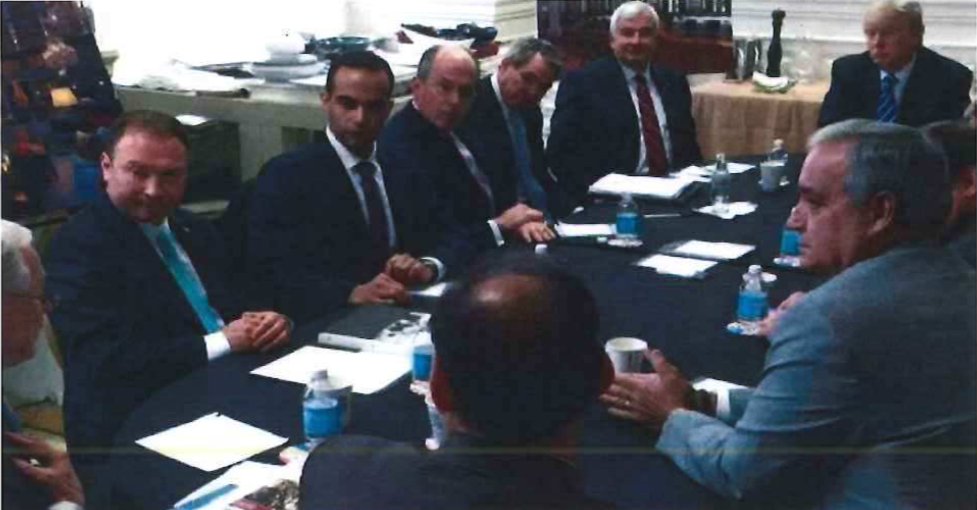
\includegraphics[width=5in]{images/p-86-foreign-policy-team.png}%
    \end{center}
    \vspace{-20pt}
    \caption*{March~31, 2016 Meeting of Foreign Policy Team, with Papadopoulos (Fourth from Right of Candidate Trump}
    \vspace{-10pt}
    \label{fig:foreign-policy-team}
\end{figure}

During the meeting, each of the newly announced foreign policy advisors introduced themselves and briefly described their areas of experience or expertise.% 435
\footnote{Papadopoulos 8/10/17 302, at 4.}
Papadopoulos spoke about his previous work in the energy sector and then brought up a potential meeting with Russian officials.% 436
\footnote{Papadopoulos 8/10/17 302, at 4.}
Specifically, Papadopoulos told the group that he had learned through his contacts in London that Putin wanted to meet with candidate Trump and that these connections could help arrange that meeting.% 437
\footnote{\textit{Papadopoulos} Statement of Offense \P 9; \textit{see} Gordon 8/29/17 302, at 14; Carafano 9/12/17 302, at 2; Hoskins 9/14/17 302, at 1.}

Trump and Sessions both reacted to Papadopoulos's statement. Papadopoulos and Campaign advisor J.D. Gordon---who told investigators in an interview that he had a "crystal clear" recollection of the meeting---have stated that Trump was interested in and receptive to the idea of a meeting with Putin.% 438
\footnote{Papadopoulos 8/10/17 302, at 4--5; Gordon 9/7/17 302, at 4--5.}
Papadopoulos understood Sessions to be similarly supportive of his efforts to arrange a meeting.% 439
\footnote{Papadopoulos 8/10/17 302, at 5; Papadopoulos 8/11/17 302, at 3.}
Gordon and two other attendees, however, recall that Sessions generally opposed the proposal, though they differ in their accounts of the concerns he voiced or the strength of the opposition he expressed.% 440
\footnote{Sessions 1/17/18 302, at 17; Gordon 9/7/17 302, at 5; Hoskins 9/14/17 302, at 1; Carafano 9/12/17 302, at 2.}

\paragraph{George Papadopoulos Learns That Russia Has "Dirt" in the Form of Clinton Emails}

Whatever Sessions's precise words at the March~31 meeting, Papadopoulos did not understand Sessions or anyone else in the Trump Campaign to have directed that he refrain from making further efforts to arrange a meeting between the Campaign and the Russian government.
To the contrary, Papadopoulos told the Office that he understood the Campaign to be supportive of his efforts to arrange such a meeting.% 441
\footnote{Papadopoulos 8/10/17 302, at 4--5; Papadopoulos 8/11/17 302, at 3; Papadopoulos 9/20/17 302, at 2.}
Accordingly, when he returned to London, Papadopoulos resumed those efforts.% 442
\footnote{\textit{Papadopoulos} Statement of Offense \P 10.}

Throughout April 2016, Papadopoulos continued to correspond with, meet with, and seek Russia contacts through Mifsud and, at times, Polonskaya.% 443
\footnote{\textit{Papadopoulos} Statement of Offense \P\P 10--15.}
For example, within a week of her initial March~24 meeting with him, Polonskaya attempted to send Papadopoulos a text message---which email exchanges show to have been drafted or edited by Mifsud---addressing Papadopoulos's "wish to engage with the Russian Federation."% 444
\footnote{3/29/16 Emails, Mifsud to Polonskaya (3:39 a.m. and 5:36 a.m.).}
When Papadopoulos learned from Mifsud that Polonskaya had tried to message him, he sent her an email seeking another meeting.% 445
\footnote{4/10/16 Email, Papadopoulos to Polonskaya (2:45:59 p.m.).}
Polonskaya responded the next day that she was "back in St. Petersburg" but "would be very pleased to support [Papadopoulos's] initiatives between our two countries" and "to meet [him] again."% 446
\footnote{4/11/16 Email, Polonskaya to Papadopoulos (3:11:24 a.m.).}
Papadopoulos stated in reply that he thought "a good step" would be to introduce him to "the Russian Ambassador in London," and that he would like to talk to the ambassador, "or anyone else you recommend, about a potential foreign policy trip to Russia."% 447
\footnote{4/11/16 Email, Papadopoulos to Polonskaya (9:21:56 a.m.).}

Mifsud, who had been copied on the email exchanges, replied on the morning of April~11, 2016.
He wrote, "This is already been agreed.
I am flying to Moscow on the 18th for a Valdai meeting, plus other meetings at the Duma.
We will talk tomorrow."% 448
\footnote{4/11/16 Email, Mifsud to Papadopoulos (11:43:53).}
The two bodies referenced by Mifsud are part of or associated with the Russian government: the Duma is a Russian legislative assembly,% 449
\footnote{Papadopoulos Statement of Offense \P 10(c).}
while "Valdai" refers to the Valdai Discussion Club, a Moscow-based group that "is close to Russia's foreign-policy establishment."% 450
\footnote{Anton Troianovski, \textit{Putin Ally Warns of Arms Race as Russia Considers Response to U.S. Nuclear Stance}, Washington Post (Feb.~10, 2018).}
Papadopoulos thanked Mifsud and said that he would see him "tomorrow."% 451
\footnote{4/11/16 Email, Papadopoulos to Mifsud (11:51:53 a.m.).}
For her part, Polonskaya responded that she had "already alerted my personal links to our conversation and your request," that "we are all very excited [about] the possibility of a good relationship with Mr.~Trump," and that "[t]he Russian Federation would love to welcome him once his candidature would be officially announced."% 452
\footnote{4/12/16 Email, Polonskaya to Papadopoulos (4:47:06 a.m.).}

Papadopoulos's and Mifsud's mentions of seeing each other "tomorrow" referenced a meeting that the two had scheduled for the next morning, April~12, 2016, at the Andaz Hotel in London.
Papadopoulos acknowledged the meeting during interviews with the Office,% 453
\footnote{Papadopoulos 9/19/17 302, at 7.}
and records from Papadopoulos's UK cellphone and his internet-search history all indicate that the meeting took place.% 454
\footnote{4/12/16 Email, Mifsud to Papadopoulos (5:44:39 a.m.) (forwarding Libya-related document); 4/12/16 Email, Mifsud to Papadopoulos \& Obaid (10:28:20 a.m.); Papadopoulos Internet Search History (Apr.~11, 2016 10:56:49 p.m.) (search for “andaz hotel liverpool street”); 4/12/16 Text Messages, Mifsud \& Papadopoulos.}

Following the meeting, Mifsud traveled as planned to Moscow.% 455
\footnote{\textit{See}, e.g., 4/18/16 Email, Mifsud to Papadopoulos (8:04:54 a.m.).}
On April~18, 2016, while in Russia, Mifsud introduced Papadopoulos over email to Ivan Timofeev, a member of the Russian International Affairs Council (RIAC).% 456
\footnote{Papadopoulos 8/10/17 302, at 5.}
Mifsud had described Timofeev as having connections with the Russian Ministry of Foreign Affairs (MFA),% 457
\footnote{\textit{Papadopoulos} Statement of Offense \P 11.}
the executive entity in Russia responsible for Russian foreign relations.% 458
\footnote{During the campaign period, Papadopoulos connected over LinkedIn with several MFA-affiliated individuals in addition to Timofeev.
On April~25, 2016, he connected with Dmitry Andreyko, publicly identified as a First Secretary at the Russian Embassy in Ireland.
In July 2016, he connected with Yuriy Melnik, the spokesperson for the Russian Embassy in Washington and with Alexey Krasilnikov, publicly identified as a counselor with the MFA\null.
And on September~16, 2016, he connected with Sergei Nalobin, also identified as an MFA official.
\textit{See} Papadopoulos LinkedIn Connections \blackout{Investigative Technique}}
Over the next several weeks, Papadopoulos and Timofeev had multiple conversations over Skype and email about setting "the groundwork" for a "potential" meeting between the Campaign and Russian government officials.% 459
\footnote{\textit{Papadopoulos} Statement of Offense \P 11.}
Papadopoulos told the Office that, on one Skype call, he believed that his conversation with Timofeev was being monitored or supervised by an unknown third party, because Timofeev spoke in an official manner and Papadopoulos heard odd noises on the line.% 460
\footnote{Papadopoulos 8/10/17 302, at 5; Papadopoulos 9/19/17 302, at 10.}
Timofeev also told Papadopoulos in an April~25, 2016 email that he had just spoken "to Igor Ivanov[,] the President of RIAC and former Foreign Minister of Russia," and conveyed Ivanov's advice about how best to arrange a "Moscow visit."% 461
\footnote{4/25/16 Email, Timofeev to Papadopoulos (8:16:35 a.m.).}

After a stop in Rome, Mifsud returned to England on April~25, 2016.% 462
\footnote{4/22/16 Email, Mifsud to Papadopoulos (12:41:01 a.m.).}
The next day, Papadopoulos met Mifsud for breakfast at the Andaz Hotel (the same location as their last meeting).% 463
\footnote{\textit{Papadopoulos} Statement of Offense \P 14;
4/25/16 Text Messages, Mifsud \& Papadopoulos.}
During that meeting, Mifsud told Papadopoulos that he had met with high-level Russian government officials during his recent trip to Moscow.
Mifsud also said that, on the trip, he learned that the Russians had obtained "dirt" on candidate Hillary Clinton.
As Papadopoulos later stated to the FBI, Mifsud said that the "dirt" was in the form of "emails of Clinton," and that they "have thousands of emails."% 464
\footnote{\textit{Papadopoulos} Statement of Offense \P 14.}
On May~6, 2016, 10 days after that meeting with Mifsud, Papadopoulos suggested to a representative of a foreign government that the Trump Campaign had received indications from the Russian government that it could assist the Campaign through the anonymous release of information that would be damaging to Hillary Clinton.% 465
\footnote{This information is contained in the FBI case-opening document and related materials.
\sout{The information is law enforcement sensitive (LES) and must be treated accordingly in any external dissemination.}
The foreign government conveyed this information to the U.S. government on July~26, 2016, a few days after WikiLeaks's release of Clinton-related emails.
The FBI opened its investigation of potential coordination between Russia and the Trump Campaign a few days later based on the information.}

\paragraph{Russia-Related Communications With The Campaign}

While he was discussing with his foreign contacts a potential meeting of campaign officials with Russian government officials, Papadopoulos kept campaign officials apprised of his efforts.
On April~25, 2016, the day before Mifsud told Papadopoulos about the emails, Papadopoulos wrote to senior policy advisor Stephen Miller that "[t]he Russian government has an open invitation by Putin for Mr.~Trump to meet him when he is ready," and that "[t]he advantage of being in London is that these governments tend to speak a bit more openly in 'neutral' cities."% 466
\footnote{4/25/16 Email, Papadopoulos to S. Miller (8:12:44 p.m.).}
On April~27, 2016, after his meeting with Mifsud, Papadopoulos wrote a second message to Miller stating that "some interesting messages [were] coming in from Moscow about a trip when the time is right."% 467
\footnote{4/27/16 Email, Papadopoulos to S. Miller (6:55:58 p.m.).}
The same day, Papadopoulos sent a similar email to campaign manager Corey Lewandowski, telling Lewandowski that Papadopoulos had "been receiving a lot of calls over the last month about Putin wanting to host [Trump] and the team when the time is right. "% 468
\footnote{4/27/16 Email, Papadopoulos to Lewandowski (7:15:14 p.m.).}

Papadopoulos's Russia-related communications with Campaign officials continued throughout the spring and summer of 2016.
On May~4, 2016, he forwarded to Lewandowski an email from Timofeev raising the possibility of a meeting in Moscow, asking Lewandowski whether that was "something we want to move forward with."% 469
\footnote{5/4/16 Email, Papadopoulos to Lewandowski (8:14:49 a.m.).}
The next day, Papadopoulos forwarded the same Timofeev email to Sam Clovis, adding to the top of the email "Russia update."% 470
\footnote{5/5/16 Email, Papadopoulos to Clovis (7:15:21 p.m.).}
He included the same email in a May~21, 2016 message to senior Campaign official Paul Manafort, under the subject line "Request from Russia to meet Mr.~Trump," stating that "Russia has been eager to meet Mr.~Trump for quite sometime and have been reaching out to me to discuss."% 471
\footnote{5/21/16 Email, Papadopoulos to Manafort (2:30:14 p.m.).}
Manafort forwarded the message to another Campaign official, without including Papadopoulos, and stated: "Let[']s discuss.
We need someone to communicate that [Trump] is not doing these trips.
It should be someone low level in the Campaign so as not to send any signal."% 472
\footnote{\textit{Papadopoulos} Statement of Offense \P 19 n.2.}

On June~1, 2016, Papadopoulos replied to an earlier email chain with Lewandowski about a Russia visit, asking if Lewandowski "want[ed] to have a call about this topic" and whether "we were following up with it."% 473
\footnote{6/1/16 Email, Papadopoulos to Lewandowski (3:08:18 p.m.).}
After Lewandowski told Papadopoulos to "connect with" Clovis because he was "running point," Papadopoulos emailed Clovis that "the Russian MFA" was asking him "if Mr.~Trump is interested in visiting Russia at some point."% 474
\footnote{6/1/16 Email, Lewandowski to Papadopoulos (3:20:03 p.m.);
6/1/16 Email, Papadopoulos to Clovis (3:29:14 p.m.).}
Papadopoulos wrote in an email that he "[w]anted to pass this info along to you for you to decide what's best to do with it and what message I should send (or to ignore)."% 475
\footnote{6/1/16 Email, Papadopoulos to Clovis (3:29:14 p.m.).
Papadopoulos's email coincided in time with another message to Clovis suggesting a Trump--Putin meeting.
First, on May~15, 2016, David Klein---a distant relative of then-Trump Organization lawyer Jason Greenblatt---emailed Clovis about a potential Campaign meeting with Berel Lazar, the Chief Rabbi of Russia.
The email stated that Klein had contacted Lazar in February about a possible Trump--Putin meeting and that Lazar was “a very close confidante of Putin.”
DJTFP00011547 (5/15/16 Email, Klein to Clovis (5:45:24 p.m.)).
The investigation did not find evidence that Clovis responded to Klein's email or that any further contacts of significance came out of Klein's subsequent meeting with Greenblatt and Rabbi Lazar at Trump Tower.
Klein 8/30/18 302, at 2.}

After several email and Skype exchanges with Timofeev,% 476
\footnote{\textit{Papadopoulos} Statement of Offense \P 21(a).}
Papadopoulos sent one more email to Lewandowski on June~19, 2016, Lewandowski's last day as campaign manager.% 477
\footnote{\blackout{Grand Jury}}
The email stated that "[t]he Russian ministry of foreign affairs" had contacted him and asked whether, if Mr.~Trump could not travel to Russia, a campaign representative such as Papadopoulos could attend meetings.% 478
\footnote{6/19/16 Email, Papadopoulos to Lewandowski (1:11:11 p.m.).}
Papadopoulos told Lewandowski that he was "willing to make the trip off the record if it's in the interest of Mr.~Trump and the campaign to meet specific people."% 479
\footnote{6/19/16 Email, Papadopoulos to Lewandowski (1:11:11 p.m.).}

Following Lewandowski's departure from the Campaign, Papadopoulos communicated with Clovis and Walid Phares, another member of the foreign policy advisory team, about an off-the-record meeting between the Campaign and Russian government officials or with Papadopoulos's other Russia connections, Mifsud and Timofeev.% 480
\footnote{\textit{Papadopoulos} Statement of Offense \P 21;
7/14/16 Email, Papadopoulos to Timofeev (11:57:24 p.m.);
7/15/16 Email, Papadopoulos to Mifsud;
7/27/16 Email, Papadopoulos to Mifsud (2:14:18 p.m.).}
Papadopoulos also interacted directly with Clovis and Phares in connection with the summit of the Transatlantic Parliamentary Group on Counterterrorism (TAG), a group for which Phares was co-secretary general.% 481
\footnote{Papadopoulos 9/19/17 302, at 16--17;
\textit{9th TAG Summit in Washington DC}, Transatlantic Parliament Group on Counter Terrorism.}
On July~16, 2016, Papadopoulos attended the TAG summit in Washington, D.C., where he sat next to Clovis (as reflected in the photograph below).% 482
\footnote{\textit{9th TAG Summit in Washington DC}, Transatlantic Parliament Group on Counter Terrorism.}

\begin{figure}[t]
    \vspace{-20pt}
    \begin{center}
        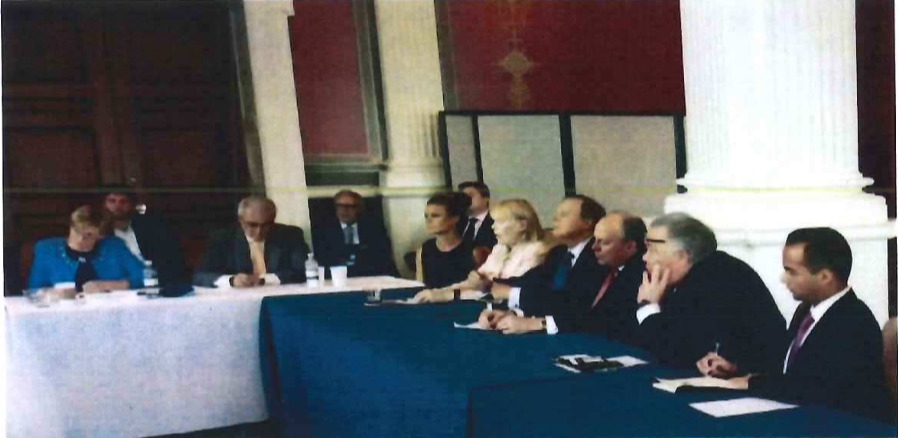
\includegraphics[width=5in]{images/p-91-papadopolous-clovis.png}%
    \end{center}
    \vspace{-20pt}
    \caption*{George Papadopoulos (far right) and Sam Clovis (second from right)}
    \vspace{-10pt}
    \label{fig:papadopolous-clovis}
\end{figure}

Although Clovis claimed to have no recollection of attending the TAG summit,% 483
\footnote{\blackout{Grand Jury}}
Papadopoulos remembered discussing Russia and a foreign policy trip with Clovis and Phares during the event.% 484
\footnote{Papadopoulos 9/19/17 302, at 16--17.}
Papadopoulos's recollection is consistent with emails sent before and after the TAG summit.
The pre-summit messages included a July~11, 2016 email in which Phares suggested meeting Papadopoulos the day after the summit to chat,% 485
\footnote{7/11/16 Email, Phares to Papadopoulos.}
and a July~12 message in the same chain in which Phares advised Papadopoulos that other summit attendees "are very nervous about Russia. So be aware."% 486
\footnote{7/12/16 Email, Phares to Papadopoulos (14:52:29).}
Ten days after the summit, Papadopoulos sent an email to Mifsud listing Phares and Clovis as other "participants" in a potential meeting at the London Academy of Diplomacy.% 487
\footnote{7/27/16 Email, Papadopoulos to Mifsud (14:14:18).}

Finally, Papadopoulos's recollection is also consistent with handwritten notes from a journal that he kept at the time.% 488
\footnote{Papadopoulos 9/20/17 302, at 3.}
Those notes, which are reprinted in part below, appear to refer to potential September 2016 meetings in London with representatives of the "office of Putin," and suggest that Phares, Clovis, and Papadopoulos ("Walid/Sam me") would attend without the official backing of the Campaign ("no official letter/no message from Trump").% 489
\footnote{Papadopoulos declined to assist in deciphering his notes, telling investigators that he could not read his own handwriting from the journal.
Papadopoulos 9/19/17 302, at 21.
The notes, however, appear to read as listed in the column to the left of the image above.}

\begin{wrapfigure}{tr}{3.1in}
    \vspace{-20pt}
    \begin{center}
        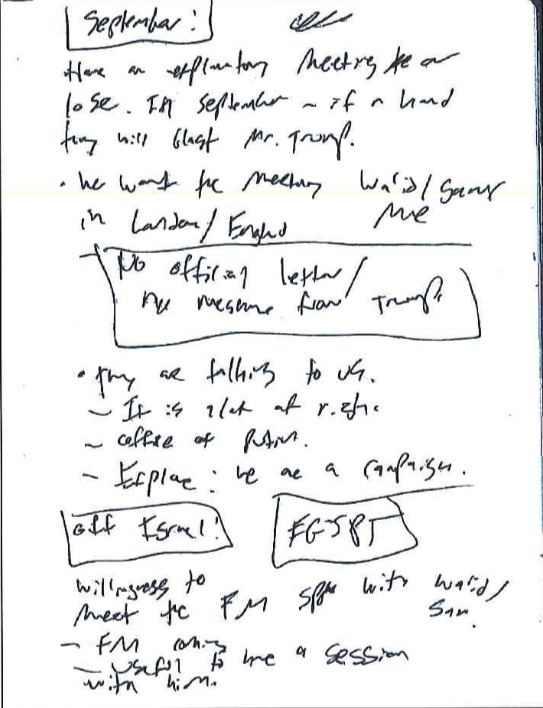
\includegraphics[width=3in]{images/p-92-papadopolous-notes.png}%
    \end{center}
    \vspace{-20pt}
    \caption*{}
    \vspace{-10pt}
    \label{fig:papadopolous-notes}
\end{wrapfigure}

\begin{quote}
September:

Have an exploratory meeting \sout{to} or lose.
In September - if allowed they will blast Mr.~Trump.

We want the meeting in London/England

Walid/Sam me

No official letter/no message from Trump

They are talking to us.

-It is a lot of risk.

-Office of Putin.

-Explore: we are a campaign.

off Israel! EGYPT

Willingness to meet the FM sp with Walid/Sam

-FM coming

-Useful to have a session with him.
\end{quote}

Later communications indicate that Clovis determined that he (Clovis) could not travel.
On August~15, 2016, Papadopoulos emailed Clovis that he had received requests from multiple foreign governments, "even Russia[]," for "closed door workshops/consultations abroad," and asked whether there was still interest for Clovis, Phares, and Papadopoulos "to go on that trip."% 490
\footnote{8/15/16 Email, Papadopoulos to Clovis (11:59:07 a.m.).}
Clovis copied Phares on his response, which said that he could not "travel before the election" but that he "would encourage [Papadopoulos] and Walid to make the trips, if it is feasible."% 491
\footnote{8/15/16 Email, Clovis to Papadopoulos (12:01:45 p.m.)}

Papadopoulos was dismissed from the Trump Campaign in early October 2016, after an interview he gave to the Russian news agency Interfax generated adverse publicity.% 492
\footnote{\textit{George Papadopoulos: Sanctions Have Done Little More Than to Turn Russia Towards China}, Interfax (Sept.~30, 2016).}

\paragraph{Trump Campaign Knowledge of "Dirt"}

Papadopoulos admitted telling at least one individual outside of the Campaign---specifically, the then-Greek foreign minister---about Russia's obtaining Clinton-related emails.% 493
\footnote{Papadopoulos 9/19/17 302, at 14--15;
Def.~Sent.~Mem., United States v.\ George Papadopoulos, 1:17-cr-182 (D.D.C. Aug.~31, 2018), Doc.~45.}
In addition, a different foreign government informed the FBI that, 10 days after meeting with Mifsud in late April 2016, Papadopoulos suggested that the Trump Campaign had received indications from the Russian government that it could assist the Campaign through the anonymous release of information that would be damaging to Hillary Clinton.% 494
\footnote{\textit{See} footnote 465 of Volume~I, Section~IV.A.2.d, \textit{supra}.}
(This conversation occurred after the GRU spearphished Clinton Campaign chairman John Podesta and stole his emails, and the GRU hacked into the DCCC and DNC, see Volume~I, Sections~III.A \& III.B, supra.)
Such disclosures raised questions about whether Papadopoulos informed any Trump Campaign official about the emails.

When interviewed, Papadopoulos and the Campaign officials who interacted with him told the Office that they could not recall Papadopoulos's sharing the information that Russia had obtained "dirt" on candidate Clinton in the form of emails or that Russia could assist the Campaign through the anonymous release of information about Clinton.
Papadopoulos stated that he could not clearly recall having told anyone on the Campaign anyone on the Campaign and wavered about whether he accurately remembered an incident in which Clovis had been upset after hearing Papadopoulos tell Clovis that Papadopoulos thought "they have her emails."% 495
\footnote{Papadopoulos 8/10/17 302, at 5;
Papadopoulos 8/11/17 302, at 5;
Papadopoulos 9/20/17 302, at 2.}
The Campaign officials who interacted or corresponded with Papadopoulos have similarly stated, with varying degrees of certainty, that he did not tell them.
Senior policy advisor Stephen Miller, for example, did not remember hearing anything from Papadopoulos or Clovis about Russia having emails of or dirt on candidate Clinton.% 496
\footnote{S. Miller 12/14/17 302, at 10.}
Clovis stated that he did not recall anyone, including Papadopoulos, having given him non-public information that a foreign government might be in possession of material damaging to Hillary Clinton.% 497
\footnote{\blackout{Grand Jury}}

\blackout{Grand Jury}% 498
\footnote{\blackout{Grand Jury}}
\blackout{Grand Jury}% 499
\footnote{\blackout{Grand Jury}}

No documentary evidence, and nothing in the email accounts or other communications facilities reviewed by the Office, shows that Papadopoulos shared this information with the Campaign.

\paragraph{Additional George Papadopoulos Contact}

The Office investigated another Russia-related contact with Papadopoulos.
The Office was not fully able to explore the contact because the individual at issue---Sergei Millian---remained out of the country since the inception of our investigation and declined to meet with members of the Office despite our repeated efforts to obtain an interview.

Papadopoulos first connected with Millian via LinkedIn on July~15, 2016, shortly after Papadopoulos had attended the TAG Summit with Clovis.% 500
\footnote{7/15/16 LinkedIn Message, Millian to Papadopoulos.}
Millian, an American citizen who is a native of Belarus, introduced himself "as president of [the] New York-based Russian American Chamber of Commerce," and claimed that through that position he had "insider knowledge and direct access to the top hierarchy in Russian politics."% 501
\footnote{7/15/16 LinkedIn Message, Millian to Papadopoulos.}
Papadopoulos asked Timofeev whether he had heard of Millian.% 502
\footnote{7/22/16 Facebook Message, Papadopoulos to Timofeev (7:40:23 p.m.);
7/26/16 Facebook Message, Papadopoulos to Timofeev (3:08:57 p.m.).}
Although Timofeev said no,% 503
\footnote{7/23/16 Facebook Message, Timofeev to Papadopoulos (4:31:37 a.m.);
7/26/16 Facebook Message, Timofeev to Papadopoulos (3:37:16 p.m.).}
Papadopoulos met Millian in New York City.% 504
\footnote{7/16/16 Text Messages, Papadopoulos \& Millian (7:55:43 p.m.).}
The meetings took place on July~30 and August~1, 2016.% 505
\footnote{7/30/16 Text Messages, Papadopoulos \& Millian (5:38 \& 6:05 p.m.);
7/31/16 Text Messages, Millian \& Papadopoulos (3:48 \& 4:18 p.m.);
8/1/16 Text Message, Millian to Papadopoulos (8:19 p.m.).}
Afterwards, Millian invited Papadopoulos to attend---and potentially speak at---two international energy conferences, including one that was to be held in Moscow in September 2016.% 506
\footnote{8/2/16 Text Messages, Millian \& Papadopoulos (3:04 \& 3:05 p.m.);
8/3/16 Facebook Messages, Papadopoulos \& Millian (4:07:37 a.m. \& 1:11:58 p.m.).}
Papadopoulos ultimately did not attend either conference.

On July~31, 2016, following his first in-person meeting with Millian, Papadopoulos emailed Trump Campaign official Bo Denysyk to say that he had been contacted "by some leaders of Russian-American voters here in the US about their interest in voting for Mr.~Trump," and to ask whether he should "put you in touch with their group (US--Russia chamber of commerce)."% 507
\footnote{7/31/16 Email, Papadopoulos to Denysyk (12:29:59 p.m.).}
Denysyk thanked Papadopoulos "for taking the initiative," but asked him to "hold off with outreach to Russian-Americans" because "too many articles" had already portrayed the Campaign, then-campaign chairman Paul Manafort, and candidate Trump as "being pro-Russian."% 508
\footnote{7/31/16 Email, Denysyk to Papadopoulos (21:54:52).}

On August~23, 2016, Millian sent a Facebook message to Papadopoulos promising that he would "share with you a disruptive technology that might be instrumental in your political work for the campaign."% 509
\footnote{8/23/16 Facebook Message, Millian to Papadopoulos (2:55:36 a.m.).}
Papadopoulos claimed to have no recollection of this matter.% 510
\footnote{Papadopoulos 9/20/17 302, at 2.}

On November~9, 2016, shortly after the election, Papadopoulos arranged to meet Millian in Chicago to discuss business opportunities, including potential work with Russian "billionaires who are not under sanctions."% 511
\footnote{11/10/16 Facebook Message, Millian to Papadopoulos (9:35:05 p.m.).}
The meeting took place on November~14, 2016, at the Trump Hotel and Tower in Chicago.% 512
\footnote{11/14/16 Facebook Message, Millian to Papadopoulos (1:32:11 a.m.).}
According to Papadopoulos, the two men discussed partnering on business deals, but Papadopoulos perceived that Millian's attitude toward him changed when Papadopoulos stated that he was only pursuing private-sector opportunities and was not interested in a job in the Administration.% 513
\footnote{Papadopoulos 9/19/17 302, at 19.}
The two remained in contact, however, and had extended online discussions about possible business opportunities in Russia.% 514
\footnote{\textit{E.g.}, 11/29/16 Facebook Messages, Papadopoulos \& Millian (5:09--5:11 p.m.);
12/7/16 Facebook Message, Millian to Papadopoulos (5:10:54 p.m.).}
The two also arranged to meet at a Washington, D.C. bar when both attended Trump's inauguration in late January 2017.% 515
\footnote{1/20/17 Facebook Messages, Papadopoulos \& Millian (4:37--4:39 a.m.).}

\subsubsection{Carter Page}

Carter Page worked for the rump Campaign from January 2016 to September 2016.
He was formally and publicly announced as a foreign policy advisor by the candidate in March 2016.% 516
\footnote{Page was interviewed by the FBI during five meetings in March 2017, before the Special Counsel's appointment.
\blackout{Grand Jury}}
Page had lived and worked in Russia, and he had been approached by Russian intelligence officers several years before he volunteered for the Trump Campaign.
During his time with the Campaign, Page advocated pro-Russia foreign policy positions and traveled to Moscow in his personal capacity.
Russian intelligence officials had formed relationships with Page in 2008 and 2013 and Russian officials may have focused on Page in 2016 because of his affiliation with the Campaign.
However, the investigation did not establish that Page coordinated with the Russian government in its efforts to interfere with the 2016 presidential election.

\paragraph{Background}

Before he began working for the Campaign in January 2016, Page had substantial prior experience studying Russian policy issues and living and working in Moscow.
From 2004 to 2007, Page was the deputy branch manager of Merrill Lynch's Moscow office.% 517
\footnote{\textit{Testimony of Carter Page, Hearing Before the U.S. House of Representatives, Permanent Select Committee on Intelligence,} 115th Cong.~40 (Nov.~2, 2017) (exhibit).}
There, he worked on transactions involving the Russian energy company Gazprom and came to know Gazprom's deputy chief financial officer, Sergey Yatsenko.% 518
\footnote{Page 3/30/17 302, at 10.}

In 2008, Page founded Global Energy Capital LLC (GEC), an investment management and advisory firm focused on the energy sector in emerging markets.% 519
\footnote{\blackout{Grand Jury}}
\blackout{Grand Jury}% 520
\footnote{\blackout{Grand Jury}}
The company otherwise had no sources of income, and Page was forced to draw down his life savings to support himself and pursue his business venture.% 521
\footnote{\blackout{Grand Jury}}
Page asked Yatsenko to work with him at GEC as a senior advisor on a contingency basis,
\blackout{Grand Jury}% 522
\footnote{Page 3/30/17 302, at 10; \blackout{Grand Jury}}

In 2008, Page met Alexander Bulatov, a Russian government official who worked at the Russian Consulate in New York.% 523
\footnote{\blackout{Grand Jury}}
Page later learned that Bulatov was a Russian intelligence officer,
\blackout{Grand Jury}% 524
\footnote{\blackout{Grand Jury}}

In 2013, Victor Podobnyy, another Russian intelligence officer working covertly in the United States under diplomatic cover, formed a relationship with Page.% 525
\footnote{\blackout{Grand Jury}; Complaint \P\P 22, 24, 32, United States v.\ Buryakov, 1:15-mj-215 (S.D.N.Y. Jan.~23, 2015), Doc.~1 “\textit{Buryakov} Complaint”).}
Podobnyy met Page at an energy symposium in New York City and began exchanging emails with him.% 526
\footnote{\textit{Buryakov} Complaint \P 34.}
Podobnyy and Page also met in person on multiple occasions, during which Page offered his outlook on the future of the energy industry and provided documents to Podobnyy about the energy business.% 527
\footnote{\textit{Buryakov} Complaint \P 34.}
In a recorded conversation on April~8, 2013, Podobnyy told another intelligence officer that Page was interested in business opportunities in Russia.% 528
\footnote{\textit{Buryakov} Complaint \P 32.}
In Podobnyy's words, Page "got hooked on Gazprom thinking that if they have a project, he could ... rise up. Maybe he can .... [I]t's obvious that he wants to earn lots of money."% 529
\footnote{\textit{Buryakov} Complaint.}
Podobnyy said that he had led Page on by "feed[ing] him empty promises" that Podobnyy would use his Russian business connections to help Page.% 530
\footnote{\textit{Buryakov} Complaint.}
Podobnyy told the other intelligence officer that his method of recruiting foreign sources was to promise them favors and then discard them once he obtained relevant information from them.% 531
\footnote{\textit{Buryakov} Complaint.}

In 2015, Podobnyy and two other Russian intelligence officers were charged with conspiracy to act as an unregistered agent of a foreign government.% 532
\footnote{\textit{See Buryakov} Complaint;
\textit{see also} Indictment, \textit{United States v.\ Buryakov}, 1:15-cr-73 (S.D.N.Y. Feb.~9, 2015), Doc.~10;
\blackout{Grand Jury}}
The criminal complaint detailed Podobnyy's interactions with and conversations about Page, who was identified only as "Male-1."% 533
\footnote{\textit{Buryakov} Complaint \P\P 32--34; \blackout{Grand Jury}}
Based on the criminal complaint's description of the interactions, Page was aware that he was the individual described as "Male-1."% 534
\footnote{\blackout{Grand Jury}}
Page later spoke with a Russian government official at the United Nations General Assembly and identified himself so that the official would understand he was "Male-1" from the Podobnyy complaint. % 535
\footnote{Page 3/16/17 302, at 4; \blackout{Grand Jury}}
Page told the official that he "didn't do anything"
\blackout{Grand Jury}% 536
\footnote{Page 3/16/17 302, at 4; \blackout{Grand Jury}}

In interviews with the FBI before the Office's opening, Page acknowledged that he understood that the individuals he had associated with were members of the Russian intelligence services, but he stated that he had only provided immaterial non-public information to them and that he did not view this relationship as a backchannel.% 537
\footnote{Page 3/30/17 302, at 6; Page 3/31/17 302, at 1}
Page told investigating agents that "the more immaterial non-public information I give them, the better for this country."% 538
\footnote{Page 3/31/17 302, at 1.}

\paragraph{Origins of and Early Campaign Work}

In January 2016, Page began volunteering on an informal, unpaid basis for the Trump Campaign after Ed Cox, a state Republican Party official, introduced Page to Trump Campaign officials.% 539
\footnote{Page 3/16/17 302, at 1; \blackout{Grand Jury}}
Page told the Office that his goal in working on the Campaign was to help candidate Trump improve relations with Russia.% 540
\footnote{Page 3/10/17 302, at 2.}
To that end, Page emailed Campaign officials offering his thoughts on U.S.--Russia relations, prepared talking points and briefing memos on Russia, and proposed that candidate Trump meet with President Vladimir Putin in Moscow.% 541
\footnote{\textit{See}, e.g., 1/30/16 Email, Page to Glassner et al.;
3/17/16 Email, Page to Clovis (attaching a “President's Daily Brief” prepared by Page that discussed the “severe degradation of U.S.--Russia relations following Washington's meddling” in Ukraine); \blackout{Grand Jury}}

In communications with Campaign officials, Page also repeatedly touted his high-level contacts in Russia and his ability to forge connections between candidate Trump and senior Russian governmental officials.
For example, on January~30, 2016, Page sent an email to senior Campaign officials stating that he had "spent the past week in Europe and ha[d] been in discussions with some individuals with close ties to the Kremlin" who recognized that Trump could have a "game-changing effect ... in bringing the end of the new Cold War."% 542
\footnote{1/30/16 Email, Page to Glassner et al.}
The email stated that "[t]hrough [his] discussions with these high level contacts," Page believed that "a direct meeting in Moscow between Mr[.] Trump and Putin could be arranged."% 543
\footnote{1/30/16 Email, Page to Glassner et al.}
Page closed the email by criticizing U.S. sanctions on Russia.% 544
\footnote{1/30/16 Email, Page to Glassner et al.}
\blackout{Grand Jury}% 545
\footnote{\blackout{Grand Jury}}

On March~21, 2016, candidate Trump formally and publicly identified Page as a member of his foreign policy team to advise on Russia and the energy sector.% 546
\footnote{\textit{A Transcript of Donald Trump's Meeting with the Washington Post Editorial Board}, Washington Post (Mar.~21, 2016); \blackout{Grand Jury}}
Over the next several months, Page continued providing policy-related work product to Campaign officials.
For example, in April 2016, Page provided feedback on an outline for a foreign policy speech that the candidate gave at the Mayflower Hotel,% 547
\footnote{\blackout{Grand Jury}}
see Volume~I, Section~IV.A.4, infra.
In May 2016, Page prepared an outline of an energy policy speech for the Campaign and then traveled to Bismarck, North Dakota, to watch the candidate deliver the speech.% 548
\footnote{\blackout{Grand Jury}}
Chief policy advisor Sam Clovis expressed appreciation for Page's work and praised his work to other Campaign officials.% 549
\footnote{\textit{See}, e.g., 3/28/16 Email, Clovis to Lewandowski et~al.\
(forwarding notes prepared by Page and stating, “I wanted to let you know the type of work some of our advisors are capable of.”).}

\paragraph{Carter Page's July 2016 Trip To Moscow}

Page's affiliation with the Trump Campaign took on a higher profile and drew the attention of Russian officials after the candidate named him a foreign policy advisor.
As a result, in late April 2016, Page was invited to give a speech at the July 2016 commencement ceremony at the New Economic School (NES) in Moscow.% 550
\footnote{Page 3/16/17 302, at 2--3; Page 3/10/17 302, at 3.}
The NES commencement ceremony generally featured high-profile speakers; for example, President Barack Obama delivered a commencement address at the school in 2009.% 551
\footnote{S. Weber 7/28/17 302, at 3.}
NES officials told the Office that the interest in inviting Page to speak at NES was based entirely on his status as a Trump Campaign advisor who served as the candidate's Russia expert.% 552
\footnote{Y. Weber 6/1/17 302, at 4--5;
S. Weber 7/28/17 302, at 3.}
Andrej Krickovic, an associate of Page's and assistant professor at the Higher School of Economics in Russia, recommended that NES rector Shlomo Weber invite Page to give the commencement address based on his connection to the Trump Campaign.% 553
\footnote{\textit{See} Y, Weber 6/1/17 302, at 4;
S. Weber 7/28/17 302, at 3.}
Denis Klimentov, an employee of NES, said that when Russians learned of Page's involvement in the Trump Campaign in March 2016, the excitement was palpable.% 554
\footnote{De, Klimentov 6/9/17 302, at 2.}
Weber recalled that in summer 2016 there was substantial interest in the Trump Campaign in Moscow, and he felt that bringing a member of the Campaign to the school would be beneficial.% 555
\footnote{S. Weber 7/28/17 302, at 3.}

Page was eager to accept the invitation to speak at NES, and he sought approval from Trump Campaign officials to make the trip to Russia.% 556
\footnote{\textit{See} 5/16/16 Email, Page to Phares et~al.\
(referring to submission of a “campaign advisor request form”).}
On May~16, 2016, while that request was still under consideration, Page emailed Clovis, J.D. Gordon, and Walid Phares and suggested that candidate Trump take his place speaking at the commencement ceremony in Moscow.% 557
\footnote{\blackout{Grand Jury}; 5/16/16 Email, Page to Phares et al.}
On June~19, 2016, Page followed up again to request approval to speak at the NES event and to reiterate that NES "would love to have Mr.~Trump speak at this annual celebration" in Page's place.% 558
\footnote{6/19/16 Email, Page to Gordon et al.}
Campaign manager Corey Lewandowski responded the same day, saying, "If you want to do this, it would be out side [sic] of your role with the DJT for President campaign. I am certain Mr.~Trump will not be able to attend.% 559
\footnote{6/19/16 Email, Lewandowski to Page et~al.}

In early July 2016, Page traveled to Russia for the NES events.
On July~5, 2016, Denis Klimentov, copying his brother, Dmitri Klimentov,% 560
\footnote{Dmitri Klimentov is a New York-based public relations consultant.}
emailed Maria Zakharova, the Director of the Russian Ministry of Foreign Affairs' Information and Press Department, about Page's visit and his connection to the Trump Campaign.% 561
\footnote{7/5/16 Email, Klimentov to Zakharova (translated).}
Denis Klimentov said in the email that he wanted to draw the Russian government's attention to Page's visit in Moscow.% 562
\footnote{7/5/16 Email, Klimentov to Zakharova (translated).}
His message to Zakharova continued: "Page is Trump's adviser on foreign policy.
He is a known businessman; he used to work in Russia ....
If you have any questions, I will be happy to help contact him."% 563
\footnote{7/5/16 Email, Klimentov to Zakharova (translated).}
Dmitri Klimentov then contacted Russian Press Secretary Dmitry Peskov about Page's visit to see if Peskov wanted to introduce Page to any Russian government officials.% 564
\footnote{De.~Klimentov 11/27/18 302, at 1--2.}
The following day, Peskov responded to what appears to have been the same Denis Klimentov--Zakharova email thread.
Peskov wrote, "I have read about [Page].
Specialists say that he is far from being the main one.
So I better not initiate a meeting in the Kremlin."% 565
\footnote{7/6/16 Email, Peskov to Klimentov (translated).}

On July~7, 2016, Page delivered the first of his two speeches in Moscow at NES.% 566
\footnote{Page 3/10/17 302, at 3.}
In the speech, Page criticized the U.S. government's foreign policy toward Russia, stating that "Washington and other Western capitals have impeded potential progress through their often hypocritical focus on ideas such as democratization, inequality, corruption and regime change."% 567
\footnote{See Carter W. Page, \textit{The Lecture of Trump's Advisor Carter Page in Moscow}, YouTube Channel Katehon Think Tank, Posted July~7, 2016,
available at https://www.youtube.com/watch?time\_continue=28\&v=1CYF29saA9w.
Page also provided the FBI with a copy of his speech and slides from the speech.
See Carter Page, “The Evolution of the World Economy: Trends and Potential,” Speech at National Economic Speech (July~7, 2016).} % XXX: New Economic School
On July~8, 2016, Page delivered a speech during the NES commencement.% 568
\footnote{Page 3/10/17 302, at 3.}
After Page delivered his commencement address, Russian Deputy Prime Minister and NES board member Arkady Dvorkovich spoke at the ceremony and stated that the sanctions the United States had imposed on Russia had hurt the NES\null.% 569
\footnote{Page 3/16/17 302, at 3.}
Page and Dvorkovich shook hands at the commencement ceremony, and Weber recalled that Dvorkovich made statements to Page about working together in the future.% 570
\footnote{S. Weber 7/28/17 302, at 4.}
\blackout{Grand Jury}% 571
\footnote{\blackout{Grand Jury}}

Page said that, during his time in Moscow, he met with friends and associates he knew from when he lived in Russia, including Andrey Baranov, a former Gazprom employee who had become the head of investor relations at Rosneft, a Russian energy company.% 572
\footnote{Page 3/10/17 302, at 3;
Page 3/30/17 302, at 3;
Page 3/31/17 302, at 2.}
Page stated that he and Baranov talked about "immaterial non-public" information.% 573
\footnote{Page 3/30/17 302, at 3.}
Page believed he and Baranov discussed Rosneft president Igor Sechin, and he thought Baranov might have mentioned the possibility of a sale of a stake in Rosneft in passing.% 574
\footnote{Page 3/30/17 302, at 9. \blackout{Grand Jury}}
Page recalled mentioning his involvement in the Trump Campaign with Baranov, although he did not remember details of the conversation.% 575
\footnote{\blackout{Grand Jury} Page 3/30/17 302, at 3.}
Page also met with individuals from Tatneft, a Russian energy company, to discuss possible business deals, including having Page work as a consultant.% 576
\footnote{Page 3/10/17 302, at 3;
Page 3/30/17 302, at 7;
Page 3/31/17 302, at 2.}

On July~8, 2016, while he was in Moscow, Page emailed several Campaign officials and stated he would send "a readout soon regarding some incredible insights and outreach I've received from a few Russian legislators and senior members of the Presidential Administration here."% 577
\footnote{\blackout{Grand Jury} 7/8/16 Email, Page to Dahl \& Gordon.}
On July~9, 2016, Page emailed Clovis, writing in pertinent part:

\begin{quote}
Russian Deputy Prime minister and NES board member Arkady Dvorkovich also spoke before the event.
In a private conversation, Dvorkovich expressed strong support for Mr.~Trump and a desire to work together toward devising better solutions in response to the vast range of current international problems.
Based on feedback from a diverse array of other sources close to the Presidential Administration, it was readily apparent that this sentiment is widely held at all levels of government.% 578
\footnote{\blackout{Grand Jury} 7/9/16 Email, Page to Clovis.}
\end{quote}

Despite these representations to the Campaign,
\blackout{Grand Jury}% 579
\footnote{\blackout{Grand Jury}}
\blackout{Grand Jury}% 580
\footnote{\blackout{Grand Jury}}
\blackout{Grand Jury}% 591
\footnote{\blackout{Grand Jury}}
\blackout{Grand Jury}% 582
\footnote{\blackout{Grand Jury}}
The Office was unable to obtain additional evidence or testimony about who Page may have met or communicated with in Moscow; thus, Page's activities in Russia---as described in his emails with the Campaign---were not fully explained.

\paragraph{Later Campaign Work and Removal from the Campaign}

In July 2016, after returning from Russia, Page traveled to the Republican National Convention in Cleveland.% 583
\footnote{Page 3/10/17 302, at 4;
Page 3/16/17 302, at 3.}
While there, Page met Russian Ambassador to the United States Sergey Kislyak; that interaction is described in Volume~I, Section~IV.A.6.a, infra.% 584
\footnote{Page 3/10/17 302, at 4;
Page 3/16/17 302, at 3.}
Page later emailed Campaign officials with feedback he said he received from ambassadors he had met at the Convention, and he wrote that Ambassador Kislyak was very worried about candidate Clinton's world views.% 585
\footnote{\blackout{Grand Jury}; 7/23/16 Email, Page to Clovis;
7/25/16 Email, Page to Gordon \& Schmitz.}
\blackout{Grand Jury}% 586
\footnote{\blackout{Grand Jury}}

Following the Convention, Page's trip to Moscow and his advocacy for pro-Russia foreign policy drew the media's attention and began to generate substantial press coverage.
The Campaign responded by distancing itself from Page, describing him as an "informal foreign policy advisor" who did "not speak for Mr.~Trump or the campaign."% 587
\footnote{\textit{See, e.g.}, Steven Mufson \& Tom Hamburger, \textit{Trump Advisor's Public Comments, Ties to Moscow Stir Unease in Both Parties}, Washington Post (Aug.~5, 2016).}
On September~23, 2016, Yahoo!\ News reported that U.S. intelligence officials were investigating whether Page had opened private communications with senior Russian officials to discuss U.S. sanctions policy under a possible Trump Administration.% 588
\footnote{Michael Isikoff, \textit{U.S. Intel Officials Probe Ties Between Trump Adviser and Kremlin}, Yahoo!\ News (Sept.~23, 2016).}
A Campaign spokesman told Yahoo!\ News that Page had "no role" in the Campaign and that the Campaign was "not aware of any of his activities, past or present."% 589
\footnote{Michael Isikoff, \textit{U.S. Intel Officials Probe Ties Between Trump Adviser and Kremlin}, Yahoo!\ News (Sept.~23, 2016);
see also 9/25/16 Email, Hicks to Conway \& Bannon (instructing that inquiries about Page should be answered with “[h]e was announced as an informal adviser in March.
Since then he has had no role or official contact with the campaign.
We have no knowledge of activities past or present and he now officially has been removed from all lists etc.”).}
On September~24, 2016, Page was formally removed from the Campaign.% 590
\footnote{Page 3/16/17 302, at 2;
\textit{see, e.g.}, 9/23/16 Email, J. Miller to Bannon \& S. Miller (discussing plans to remove Page from the campaign).}

Although Page had been removed from the Campaign, after the election he sought a position in the Trump Administration.% 591
\footnote{\blackout{Grand Jury}, “Transition Online Form,” 11/14/16 (\blackout{Grand Jury})}
On November~14, 2016, he submitted an application to the Transition Team that inflated his credentials and experiences, stating that in his capacity as a Trump Campaign foreign policy advisor he had met with "top world leaders" and "effectively responded to diplomatic outreach efforts from senior government officials in Asia, Europe, the Middle East, Africa, [and] the Americas."% 592
\footnote{\blackout{Grand Jury} “Transition Online Form,” 11/14/16 \blackout{Grand Jury}}
Page received no response from the Transition Team.
When Page took a personal trip to Moscow in December 2016, he met again with at least one Russian government official.
That interaction and a discussion of the December trip are set forth in Volume~I, Section~IV.B.6, infra.

\subsubsection{Dimitri Simes and the Center for the National Interest}

Members of the Trump Campaign interacted on several occasions with the Center for the National Interest (CNI), principally through its President and Chief Executive Officer, Dimitri Simes.
CNI is a think tank with expertise in and connections to the Russian government.
Simes was born in the former Soviet Union and immigrated to the United States in the 1970s.
In April 2016, candidate Trump delivered his first speech on foreign policy and national security at an event hosted by the National Interest, a publication affiliated with CNI\null.
Then-Senator Jeff Sessions and Russian Ambassador Kislyak both attended the event and, as a result, it gained some attention in relation to Sessions's confirmation hearings to become Attorney General.
Sessions had various other contacts with CNI during the campaign period on foreign-policy matters, including Russia.
Jared Kushner also interacted with Simes about Russian issues during the campaign.
The investigation did not identify evidence that the Campaign passed or received any messages to or from the Russian government through CNI or Simes.

\paragraph{CNI and Dimitri Simes Connect with the Trump Campaign}

CNI is a Washington-based non-profit organization that grew out of a center founded by former President Richard Nixon.% 593
\footnote{Simes 3/8/18 302, at 1--2.}
CNI describes itself "as a voice for strategic realism in U.S. foreign policy," and publishes a bi-monthly foreign policy magazine, the National Interest.% 594
\footnote{\textit{About the Center}, CNI, available at https://cftni.org/about/.}
CNI is overseen by a board of directors and an advisory council that is largely honorary and whose members at the relevant time included Sessions, who served as an advisor to candidate Trump on national security and foreign policy issues.% 595
\footnote{Advisory Counsel, CNI, available at
https://web.archive.org/web/20161030025331/http://cftni.org/about/advisory-council/;
Simes 3/8/18 302, at 3--4;
Saunders 2/15/18 302, at 4;
Sessions 1/17/18 302, at 16.}

Dimitri Simes is president and CEO of CNI and the publisher and CEO of the National Interest.% 596
\footnote{Simes 3/8/18 302, at 2.}
Simes was born in the former Soviet Union, emigrated to the United States in the early 1970s, and joined CNI's predecessor after working at the Carnegie Endowment for International Peace.% 597
\footnote{ Simes 3/8/18 302, at 1--2;
Simes 3/27/18 302, at 19.}
Simes personally has many contacts with current and former Russian government officials,% 598
\footnote{Simes 3/27/18 302, at 10--15.}
as does CNI collectively.
As CNI stated when seeking a grant from the Carnegie Corporation in 2015, CNI has "unparalleled access to Russian officials and politicians among Washington think tanks,"% 599
\footnote{C00011656 (\textit{Rethinking U.S.--Russia Relations}, CNI (Apr.~18, 2015)).}
in part because CNI has arranged for U.S. delegations to visit Russia and for Russian delegations to visit the United States as part of so-called "Track 11" diplomatic efforts.% 600
\footnote{Simes 3/8/18 302, at 5;
Saunders 2/15/18 302, at 29--30;
Zakheim 1/25/18 302, at 3.}

On March~14, 2016, CNI board member Richard Plepler organized a luncheon for CNI and its honorary chairman, Henry Kissinger, at the Time Warner Building in New York.% 601
\footnote{Simes 3/8/18 302, at 6;
CO0006784 (3/11/16 Email, Gilbride to Saunders (3:43:12 p.m.);
\textit{cf.}~Zakheim 1/25/18 302, at 1 (Kissinger was CNI's “Honorary Chairman of the Board”);
Boyd 1/24/18 302, at 2;
P. Sanders 2/15/18 302, at 5.}
The idea behind the event was to generate interest in CNI's work and recruit new board members for CNI\null.% 602
\footnote{Simes 3/8/18 302, at 5--6; Simes 3/27/18 302, at 2.}
Along with Simes, attendees at the event included Jared Kushner, son-in-law of candidate Trump.% 603
\footnote{Simes 3/8/18 302, at 6; Kushner 4/11/18 302, at 2.}
Kushner told the Office that the event came at a time when the Trump Campaign was having trouble securing support from experienced foreign policy professionals and that, as a result, he decided to seek Simes's assistance during the March~14 event.% 604
\footnote{Kushner 4/11/18 302, at 2.}

Simes and Kushner spoke again on a March~24, 2016 telephone call,% 605
\footnote{Simes 3/8/18 302, at 6--7.}
three days after Trump had publicly named the team of foreign policy advisors that had been put together on short notice.% 606
\footnote{\blackout{Grand Jury} \textit{see} Volume~I, Section~IV.A.2, \textit{supra}.}
On March~31, 2016, Simes and Kushner had an in-person, one-on-one meeting in Kushner's New York office.% 607
\footnote{Simes 3/8/18 302, at 7--9.}
During that meeting, Simes told Kushner that the best way to handle foreign-policy issues for the Trump Campaign would be to organize an advisory group of experts to meet with candidate Trump and develop a foreign policy approach that was consistent with Trump's voice.% 608
\footnote{Simes 3/8/18 302, at 7--8.}
Simes believed that Kushner was receptive to that suggestion.% 609
\footnote{Simes 3/8/18 302, at 8;
\textit{see also} Boyd 1/24/18 302, at 2.}

Simes also had contact with other individuals associated with the Trump Campaign regarding the Campaign's foreign policy positions.
For example, on June~17, 2016, Simes sent J.D. Gordon an email with a "memo to Senator Sessions that we discussed at our recent meeting" and asked Gordon to both read it and share it with Sessions.
The memorandum proposed building a "small and carefully selected group of experts" to assist Sessions with the Campaign, operating under the assumption "that Hillary Clinton is very vulnerable on national security and foreign policy issues."
The memorandum outlined key issues for the Campaign, including a "new beginning with Russia."% 610
\footnote{C00008187 (6/17/16 Email, Simes to Gordon (3:35:45 p.m.)).}

\paragraph{National Interest Hosts a Foreign Policy Speech at the Mayflower Hotel}

During both their March~24 phone call and their March~31 in-person meeting, Simes and Kushner discussed the possibility of CNI hosting a foreign policy speech by candidate Trump.% 611
\footnote{Simes 3/8/18 302, at 7.}
Following those conversations, Simes agreed that he and others associated with CNI would provide behind-the-scenes input on the substance of the foreign-policy speech and that CNI officials would coordinate the logistics of the speech with Sessions and his staff, including Sessions's chief of staff, Rick Dearborn.% 612
\footnote{Simes 3/8/18 302, at 8--11;
C00008923 (4/6/16 Email, Simes to Burt (2:22:28 p.m.));
Burt 2/9/18 302, at 7.}

In mid-April 2016, Kushner put Simes in contact with senior policy advisor Stephen Miller and forwarded to Simes an outline of the foreign-policy speech that Miller had prepared.% 613
\footnote{C00008551 (4/17/16 Email, Kushner to Simes (2:44:25 p.m.));
C00006759 (4/14/16 Email Kushner to Simes \& S. Miller (12:30 p.m.)).}
Simes sent back to the Campaign bullet points with ideas for the speech that he had drafted with CNI Executive Director Paul Saunders and board member Richard Burt.% 614
\footnote{Burt 2/9/18 302, at 7;
Saunders 2/15/18 302, at 7--8.}
Simes received subsequent draft outlines from Miller, and he and Saunders spoke to Miller by phone about substantive changes to the speech.% 615
\footnote{Simes 3/8/18 302, at 13;
Saunders 2/15/18 302, at 7--8.}
It is not clear, however, whether CNI officials received an actual draft of the speech for comment; while Saunders recalled having received an actual draft, Simes did not, and the emails that CNI produced to this Office do not contain such a draft.% 616
\footnote{Simes 3/8/18 302, at 13;
Saunders 2/15/18 302, at 7--8.}

After board members expressed concern to Simes that CNI's hosting the speech could be perceived as an endorsement of a particular candidate, CNI decided to have its publication, the National Interest, serve as the host and to have the event at the National Press Club.% 617
\footnote{Saunders 2/15/18 302, at 8;
Simes 3/8/18 302, at 12;
CO00003834-43 (4/22/16 Email, Simes to Boyd et~al.\ (8:47 a.m.)).}
Kushner later requested that the event be moved to the Mayflower Hotel, which was another venue that Simes had mentioned during initial discussions with the Campaign, in order to address concerns about security and capacity.% 618
\footnote{Simes 3/8/18 302, at 12, 18;
Saunders 2/15/18 302, at 11.}

On April~25, 2016, Saunders booked event rooms at the Mayflower to host both the speech and a VIP reception that was to be held beforehand.% 619
\footnote{Saunders 2/15/18 302, at 11--12;
CO0006651-57 (Mayflower Group Sales Agreement).}
Saunders understood that the reception---at which invitees would have the chance to meet candidate Trump---would be a small event.% 620
\footnote{Saunders 2/15/18 302, at 12--13.}
Saunders decided who would attend by looking at the list of CNI's invitees to the speech itself and then choosing a subset for the reception.% 621
\footnote{Saunders 2/15/18 302, at 12.}
CNI's invitees to the reception included Sessions and Kislyak.% 622
\footnote{C00002575 (Attendee List);
C00008536 (4/25/16 Email, Simes to Kushner (4:53:45 p.m.)).}
The week before the speech Simes had informed Kislyak that he would be invited to the speech, and that he would have the opportunity to meet Trump.% 623
\footnote{Simes 3/8/18 302, at 19--20.}

When the pre-speech reception began on April~27, a receiving line was quickly organized so that attendees could meet Trump.% 624
\footnote{Simes 3/8/18 302, at 21.}
Sessions first stood next to Trump to introduce him to the members of Congress who were in attendance.% 625
\footnote{Simes 3/8/18 302, at 21.}
After those members had been introduced, Simes stood next to Trump and introduced him to the CNI invitees in attendance, including Kislyak.% 626
\footnote{Simes 3/8/18 302, at 21.}
Simes perceived the introduction to be positive and friendly, but thought it clear that Kislyak and Trump had just met for the first time.% 627
\footnote{Simes 3/8/18 302, at 21.}
Kislyak also met Kushner during the pre-speech reception.
The two shook hands and chatted for a minute or two, during which Kushner recalled Kislyak saying, "we like what your candidate is saying ... it's refreshing."% 628
\footnote{Kushner 4/11/18 302, at 4.}

Several public reports state that, in addition to speaking to Kushner at the pre-speech reception, Kislyak also met or conversed with Sessions at that time.% 629
\footnote{\textit{See, e.g.}, Ken Dilanian, \textit{Did Trump, Kushner, Sessions Have an Undisclosed Meeting With Russian?}, NBC News (June~1, 2016);
Julia Ioffe, \textit{Why Did Jeff Sessions Really Meet With Sergey Kislyak}, The Atlantic (June~13, 2017).}
Sessions stated to investigators, however, that he did not remember any such conversation.% 630
\footnote{Sessions 1/17/18 302, at 22.}
Nor did anyone else affiliated with CNI or the National Interest specifically recall a conversation or meeting between Sessions and Kislyak at the pre-speech reception.% 631
\footnote{Simes 3/8/18 302, at 21;
Saunders 2/15/18 302, at 14, 21;
Boyd 1/24/18 302, at 3--4;
Heilbrunn 2/1/18 302, at 6;
\textit{Statement Regarding President Trump's April~27, 2016 Foreign Policy Speech at the Center for the National Interest}, CNI (Mar.~8, 2017).}
It appears that, if a conversation occurred at the pre-speech reception, it was a brief one conducted in public view, similar to the exchange between Kushner and Kislyak.

The Office found no evidence that Kislyak conversed with either Trump or Sessions after the speech, or would have had the opportunity to do so.
Simes, for example, did not recall seeing Kislyak at the post-speech luncheon,% 632
\footnote{Simes 3/8/18 302, at 22;
Heilbrunn 2/1/18 302, at 7.}
and the only witness who accounted for Sessions's whereabouts stated that Sessions may have spoken to the press after the event but then departed for Capitol Hill.% 633
\footnote{Luff 1/30/18 302, at 4.}
Saunders recalled, based in part on a food-related request he received from a Campaign staff member, that Trump left the hotel a few minutes after the speech to go to the airport.% 634
\footnote{Saunders 2/15/18 302, at 15.}

\paragraph{Jeff Sessions's Post-Speech Interactions with CNI}

In the wake of Sessions's confirmation hearings as Attorney General, questions arose about whether Sessions's campaign-period interactions with CNI apart from the Mayflower speech included any additional meetings with Ambassador Kislyak or involved Russian-related matters.
With respect to Kislyak contacts, on May~23, 2016, Sessions attended CNI's Distinguished Service Award dinner at the Four Seasons Hotel in Washington, D.C.% 635
\footnote{Sessions 1/17/18 302, at 22;
Saunders 2/15/18 302, at 17.}
Sessions attended a pre-dinner reception and was seated at one of two head tables for the event.% 636
\footnote{Saunders 2/15/18 302, at 17;
C00004779-80 (5/23/16 Email, Cantelmo to Saunders \& Hagberg (9:30:12 a.m.);
C00004362 (5/23/16 Email, Bauman to Cantelmo et al.\ (2:02:32 a.m.).}
A seating chart prepared by Saunders indicates that Sessions was scheduled to be seated next to Kislyak, who appears to have responded to the invitation by indicating he would attend the event.% 637
\footnote{C00004362 (5/23/16 Email Bauman to Cantelmo et al.\ (2:02:32 a.m.).}
Sessions, however, did not remember seeing, speaking with, or sitting next to Kislyak at the dinner.% 638
\footnote{Sessions 1/17/18 302, at 22.}
Although CNI board member Charles Boyd said he may have seen Kislyak at the dinner,% 639
\footnote{Boyd 1/24/18 302, at 4.}
Simes, Saunders, and Jacob Heilbrunn---editor of the National Interest---all had no recollection of seeing Kislyak at the May~23 event.% 640
\footnote{Simes 3/8/18 302, at 23;
Saunders 2/15/18 302, at 18;
Heilbrunn 2/1/18 302, at 7.}
Kislyak also does not appear in any of the photos from the event that the Office obtained.

In the summer of 2016, CNI organized at least two dinners in Washington, D.C. for Sessions to meet with experienced foreign policy professionals.% 641
\footnote{Simes 3/8/18 302, at 31;
Saunders 2/15/18 302, at 19;
Burt 2/9/18 302, at 9--10;
Khalilzad 1/9/18 302, at 5.}
The dinners included CNI-affiliated individuals, such as Richard Burt and Zalmay Khalilzad, a former U.S. ambassador to Afghanistan and Iraq and the person who had introduced Trump before the April~27, 2016 foreign-policy speech.% 642
\footnote{Burt 2/9/18 302, at 9--10;
Khalilzad 1/9/18 302, at 1--2, 5.}
Khalilzad also met with Sessions one-on-one separately from the dinners.% 643
\footnote{Khalilzad 1/9/18 302, at 5--6.}
At the dinners and in the meetings, the participants addressed U.S. relations with Russia, including how U.S. relations with NATO and European countries affected U.S. policy toward Russia.% 644
\footnote{Simes 3/8/18 302, at 31;
Burt 2/9/18 302, at 9--10;
Khalilzad 1/9/18 302, at 5.}
But the discussions were not exclusively focused on Russia.% 645
\footnote{Saunders 2/15/18 302, at 20.}
Khalilzad, for example, recalled discussing "nation-building" and violent extremism with Sessions.% 646
\footnote{Khalilzad 1/9/18 302, at 6.}
In addition, Sessions asked Saunders (of CNI) to draft two memoranda not specific to Russia: one on Hillary Clinton's foreign policy shortcomings and another on Egypt.% 647
\footnote{Saunders 2/15/18 302, at 19--20.}

\paragraph{Jared Kushner's Continuing Contacts with Simes}

Between the April 2016 speech at the Mayflower Hotel and the presidential election, Jared Kushner had periodic contacts with Simes.% 648
\footnote{Simes 3/8/18 302, at 27.}
Those contacts consisted of both in-person meetings and phone conversations, which concerned how to address issues relating to Russia in the Campaign and how to move forward with the advisory group of foreign policy experts that Simes had proposed.% 649
\footnote{Simes 3/8/18 302, at 27.}
Simes recalled that he, not Kushner, initiated all conversations about Russia, and that Kushner never asked him to set up back-channel conversations with Russians.% 650
\footnote{Simes 3/8/18 302, at 27.}
According to Simes, after the Mayflower speech in late April, Simes raised the issue of Russian contacts with Kushner, advised that it was bad optics for the Campaign to develop hidden Russian contacts, and told Kushner both that the Campaign should not highlight Russia as an issue and should handle any contacts with Russians with care.% 651
\footnote{Simes 3/8/18 302, at 27.
During this period of time, the Campaign received a request for a high level Campaign official to meet with an officer at a Russian state-owned bank “to discuss an offer [that officer] claims to be carrying from President Putin to meet with” candidate Trump.
NOSC00005653 (5/17/16 Email, Dearborn to Kushner (8:12 a.m.)).
Copying Manafort and Gates, Kushner responded, “Pass on this.
A lot of people come claiming to carry messages.
Very few are able to verify.
For now I think we decline such meetings.
Most likely these people go back home and claim they have special access to gain importance for themselves.
Be careful.”
NOSC00005653 (5/17/16 Email, Kushner to Dearborn).}
Kushner generally provided a similar account of his interactions with Simes.% 652
\footnote{Kushner 4/11/18 302, at 11--13.}

Among the Kushner--Simes meetings was one held on August~17, 2016, at Simes's request, in Kushner's New York office.
The meeting was to address foreign policy advice that CNI was providing and how to respond to the Clinton Campaign's Russia-related attacks on candidate Trump.% 653
\footnote{Simes 3/8/18 302, at 29--30;
Simes 3/27/18 302, at 6;
Kushner 4/11/18 302, at 12;
C00007269 (8/10/16 Meeting Invitation, Vargas to Simes et~al.);
DJTFP00023484 (8/11/16 Email, Hagan to Manafort (5:57:15 p.m.)).}
In advance of the meeting, Simes sent Kushner a "Russia Policy Memo" laying out "what Mr.~Trump may want to say about Russia."% 654
\footnote{€00007981-84 (8/9/16 Email, Simes to Kushner (6:09:21 p.m.)).
The memorandum recommended “downplaying Russia as a U.S. foreign policy priority at this time” and suggested that “some tend to exaggerate Putin's flaws.”
The memorandum also recommended approaching general Russian related questions in the framework of “how to work with Russia to advance important U.S. national interests” and that a Trump Administration “not go abroad in search of monsters to destroy.”
The memorandum did not discuss sanctions but did address how to handle Ukraine-related questions, including questions about Russia's invasion and annexation of Crimea.}
In a cover email transmitting that memo and a phone call to set up the meeting, Simes mentioned "a well-documented story of highly questionable connections between Bill Clinton" and the Russian government, "parts of [which]" (according to Simes) had even been "discussed with the CIA and the FBI in the late 1990s and shared with the [Independent Counsel] at the end of the Clinton presidency."% 655
\footnote{C00007981 (8/9/16 Email, Simes to Kushner (6:09:21 p.m.)).}
Kushner forwarded the email to senior Trump Campaign officials Stephen Miller, Paul Manafort, and Rick Gates, with the note "suggestion only."% 656
\footnote{DJTFP00023459 (8/10/16 Email, Kushner to S. Miller et al.\ (11:30:13 a.m.)).}
Manafort subsequently forwarded the email to his assistant and scheduled a meeting with Simes.% 657
\footnote{DJTFP00023484 (8/11/16 Email, Hagan to Manafort (5:57:15 p.m.)).}
(Manafort was on the verge of leaving the Campaign by the time of the scheduled meeting with Simes, and Simes ended up meeting only with Kushner).

During the August~17 meeting, Simes provided Kushner the Clinton-related information that he had promised.% 658
\footnote{Simes 3/8/18 302, at 29--30;
Simes 3/27/18 302, at 6;
Kushner 4/11/18 302, at 12.}
Simes told Kushner that,
\blackout{Personal Privacy}% 659
\footnote{Simes 3/8/18 302, at 30;
Simes 3/27/18 302, at 6.}
Simes claimed that he had received this information from former CIA and Reagan White House official Fritz Ermarth, who claimed to have learned it from U.S. intelligence sources, not from Russians.% 660
\footnote{Simes 3/8/18 302, at 30.}

Simes perceived that Kushner did not find the information to be of interest or use to the Campaign because it was, in Simes's words, "old news."% 661
\footnote{Simes 3/8/18 302, at 30;
Simes 3/27/18 302, at 6.}
When interviewed by the Office, Kushner stated that he believed that there was little chance of something new being revealed about the Clintons given their long career as public figures, and that he never received from Simes information that could be "operationalized" for the Trump Campaign.% 662
\footnote{Kushner 4/11/18 302, at 12.}
Despite Kushner's reaction, Simes believed that he provided the same information at a small group meeting of foreign policy experts that CNI organized for Sessions.% 663
\footnote{Simes 3/8/18 302, at 30.}

\subsubsection{June~9, 2016 Meeting at Trump Tower}

On June~9, 2016, senior representatives of the Trump Campaign met in Trump Tower with a Russian attorney expecting to receive derogatory information about Hillary Clinton from the Russian government.
The meeting was proposed to Donald Trump~Jr.\ in an email from Robert Goldstone, at the request of his then-client Emin Agalarov, the son of Russian real-estate developer Aras Agalarov.
Goldstone relayed to Trump~Jr.\ that the "Crown prosecutor of Russia ... offered to provide the Trump Campaign with some official documents and information that would incriminate Hillary and her dealings with Russia" as "part of Russia and its government's support for Mr.~Trump."
Trump~Jr.\ immediately responded that "if it's what you say I love it," and arranged the meeting through a series of emails and telephone calls.

Trump~Jr.\ invited campaign chairman Paul Manafort and senior advisor Jared Kushner to attend the meeting, and both attended.
Members of the Campaign discussed the meeting before it occurred, and Michael Cohen recalled that Trump~Jr.\ may have told candidate Trump about an upcoming meeting to receive adverse information about Clinton, without linking the meeting to Russia.
According to written answers submitted by President Trump, he has no recollection of learning of the meeting at the time, and the Office found no documentary evidence showing that he was made aware of the meeting---or its Russian connection-before it occurred.

The Russian attorney who spoke at the meeting, Natalia Veselnitskaya, had previously worked for the Russian government and maintained a relationship with that government throughout this period of time.
She claimed that funds derived from illegal activities in Russia were provided to Hillary Clinton and other Democrats.
Trump~Jr.\ requested evidence to support those claims, but Veselnitskaya did not provide such information.
She and her associates then turned to a critique of the origins of the Magnitsky Act, a 2012 statute that imposed financial and travel sanctions on Russian officials and that resulted in a retaliatory ban on adoptions of Russian children.
Trump~Jr.\ suggested that the issue could be revisited when and if candidate Trump was elected.
After the election, Veselnitskaya made additional efforts to follow up on the meeting, but the Trump Transition Team did not engage.

\paragraph{Setting Up the June~9 Meeting}

\subparagraph{Outreach to Donald Trump~Jr}

Aras Agalarov is a Russian real-estate developer with ties to Putin and other members of the Russian government, including Russia's Prosecutor General, Yuri Chaika.% 664
\footnote{\blackout{Grand Jury} Goldstone 2/8/18 302, at 4.}
Aras Agalarov is the president of the Crocus Group, a Russian enterprise that holds substantial Russian government construction contracts and that---as discussed above, Volume~I, Section~IV.A.I, supra---worked with Trump in connection with the 2013 Miss Universe pageant in Moscow and a potential Trump Moscow real-estate project.% 665
\footnote{\blackout{Grand Jury} Kaveladze 11/16/17 302, at 3;
Shugart 9/25/17 302, at 2--3;
\blackout{Grand Jury}}
The relationship continued over time, as the parties pursued the Trump Moscow project in 2013--2014 and exchanged gifts and letters in 2016.% 666
\footnote{\blackout{Grand Jury} Goldstone 2/8/18 302, at 10;
\blackout{Grand Jury} Kaveladze 11/16/17 302, at 5--6;
4/25/16 Email, Graff to Goldstone.}
For example, in April 2016, Trump responded to a letter from Aras Agalarov with a handwritten note.% 667
\footnote{RG000033-34 (4/25/16 Email, Graff to Goldstone (attachment).}
Aras Agalarov expressed interest in Trump's campaign, passed on "congratulations" for winning in the primary and---according to one email drafted by Goldstone---an "offer" of his "support and that of many of his important Russian friends and colleagues[,] especially with reference to U.S./Russian relations."% 668
\footnote{DJTJROO008 (2/29/16 Email, Goldstone to Trump~Jr.\ et~al.);
\blackout{Grand Jury}}

On June~3, 2016, Emin Agalarov called Goldstone, Emin's then-publicist.% 669
\footnote{Call Records of Robert Goldstone \blackout{Grand Jury} Goldstone 2/8/18 302, at 6.}
Goldstone is a music and events promoter who represented Emin Agalarov from approximately late 2012 until late 2016.% 670
\footnote{Goldstone 2/8/18 302, at 1--2; \blackout{Grand Jury} Beniaminov 1/6/18 302, at 3.}
While representing Emin Agalarov, Goldstone facilitated the ongoing contact between the Trumps and the Agalarovs---including an invitation that Trump sent to Putin to attend the 2013 Miss Universe Pageant in Moscow.% 671
\footnote{Goldstone 2/8/18 302, at 1--5; \blackout{Grand Jury}
DJTJRO0008 (2/29/19 Email, Goldstone to Trump~Jr.);
Beniaminov 1/6/18 302, at 3;
Shugart 9/25/17 302, at 2;
TRUMPORG\_18\_001325 (6/21/13 Email, Goldstone to Graff);
TRUMPORG\_18\_001013 (6/24/13 Email, Goldstone to Graff);
TRUMPORG\_18\_001014 (6/24/13 Email, Graff to Shugart);
TRUMPORG\_18\_001018 (6/26/13 Email, Graff to Goldstone);
TRUMPORG\_18\_001022 (6/27/13 Email, Graff to L. Kelly);
TRUMPORG\_18\_001333 (9/12/13 Email, Goldstone to Graff, Shugart);
MU000004289 (7/27/13 Email, Goldstone to Graff, Shugart).}
\blackout{Grand Jury}% 672
\footnote{\blackout{Grand Jury} \textit{see} Goldstone 2/8/18 302, at 6--7.}
Goldstone understood
\blackout{Grand Jury}
a Russian political connection, and Emin Agalarov indicated that the attorney was a prosecutor.% 673
\footnote{\blackout{Grand Jury}}
Goldstone recalled that the information that might interest the Trumps involved Hillary Clinton
\blackout{Grand Jury}% 674
\footnote{\blackout{Grand Jury}}
\blackout{Grand Jury}% 675
\footnote{\blackout{Grand Jury}}

The \blackout{Grand Jury} mentioned by Emin Agalarov was Natalia Veselnitskaya.% 676
\footnote{In December 2018, a grand jury in the Southern District of New York returned an indictment charging Veselnitskaya with obstructing the Prevezon litigation discussed in the text above.
\textit{See} Indictment, \textit{United States v.\ Natalia Vladimirovna Veselnitskaya}, No.~18-cr-904 (S.D.N.Y.).
The indictment alleges, among other things, that Veselnitskaya lied to the district court about her relationship to the Russian Prosecutor General's Office and her involvement in responding to a U.S. document request sent to the Russian government.}
From approximately 1998 until 2001, Veselnitskaya worked as a prosecutor for the Central Administrative District of the Russian Prosecutor's Office,% 677
\footnote{Veselnitskaya 11/20/17 Statement to the Senate Committee on the Judiciary, at 2;
\blackout{Grand Jury}
}
and she continued to perform government-related work and maintain ties to the Russian government following her departure.% 678
\footnote{Testimony of Natalia Veselnitskaya Before the Senate Committee on Judiciary (Nov.~20, 2017) at 33;
Keir Simmons \& Rachel Elbaum, \textit{Russian Lawyer Veselnitskaya Says She Didn't Give Trump~Jr.\ Info on Clinton}, NBC News (July~11, 2017);
Maria Tsvetkova \& Jack Stubbs, \textit{Moscow Lawyer Who Met Trump~Jr.\ Had Russian Spy Agency As Client}, Reuters (July~21, 2017);
Andrew E. Kramer \& Sharon LaFraniere, \textit{Lawyer Who Was Said to Have Dirt on Clinton Had Closer Ties to Kremlin than She Let On}, New York Times (Apr.~27, 2018).}
She lobbied and testified about the Magnitsky Act, which imposed financial sanctions and travel restrictions on Russian officials and which was named for a Russian tax specialist who exposed a fraud and later died in a Russian prison.% 679
\footnote{\textit{See} Pub.\ L. No.~112-208 \S\S 402, 404(a)(1), 126 Stat.~1502, 1502--1506.
Sergei Magnitsky was a Russian tax specialist who worked for William Browder, a former investment fund manager in Russia.
Browder hired Magnitsky to investigate tax fraud by Russian officials, and Magnitsky was charged with helping Browder embezzle money.
After Magnitsky died in a Russian prison, Browder lobbied Congress to pass the Magnitsky Act.
\textit{See, e.g}, Andrew E. Kramer, \textit{Turning Tables in Magnitsky Case, Russia Accuses Nemesis of Murder}, New York Times (Oct.~22, 2017);
Testimony of Natalia Veselnitskaya Before the Senate Committee on Judiciary (Nov.~20, 2017), Exhibits at 1--4;
Rosie Gray, \textit{Bill Browder's Testimony to the Senate Judiciary Committee}, The Atlantic (July~25, 2017).}
Putin called the statute "a purely political, unfriendly act," and Russia responded by barring a list of current and former U.S. officials from entering Russia and by halting the adoption of Russian children by U.S. citizens.% 680
\footnote{Rilen Barry, \textit{Russia Bars 18 Americans After Sanctions by US}, New York Times (Apr.~13, 2013);
Tom Porter, \textit{Supporters of the Magnitsky Act Claim They've Been Targets of Russian Assassination and Kidnapping Bids}, Newsweek (July~16, 2017).}
Veselnitskaya performed legal work for Denis Katsyv,% 681
\footnote{Testimony of Natalia Veselnitskaya Before the Senate Committee on Judiciary (Nov.~20, 2017), at 21.}
the son of Russian businessman Peter Katsyv, and for his company Prevezon Holdings Ltd., which was a defendant in a civil-forfeiture action alleging the laundering of proceeds from the fraud exposed by Magnitsky.% 682
\footnote{\textit{See} Veselnitskaya Decl., \textit{United States v.\ Prevezon Holdings}, Ltd., No.~13-cv-6326 (S.D.N.Y.);
\textit{see Prevezon Holdings}, Second Amended Complaint;
\textit{Prevezon Holdings}, Mem.\ and Order;
\textit{Prevezon Holdings}, Deposition of Oleg Lurie.}
She also appears to have been involved in an April 2016 approach to a U.S. congressional delegation in Moscow offering "confidential information" from "the Prosecutor General of Russia" about "interactions between certain political forces in our two countries."% 683
\footnote{\textit{See} Gribbin 8/31/17 302, at 1--2 \& 1A (undated one-page document given to congressional delegation).
The Russian Prosecutor General is an official with broad national responsibilities in the Russian legal system.
\textit{See Federal Law on the Prosecutor's Office of the Russian Federation} (1992, amended 2004).}

Shortly after his June~3 call with Emin Agalarov, Goldstone emailed Trump~Jr.% 684
\footnote{RG000061 (6/3/16 Email, Goldstone to Trump~Jr.);
DJTJRO0446 (6/3/16 Email, Goldstone to Donald Trump~Jr.);
\@DonaldJTrumpJr 07/11/17 (11:00) Tweet.}
The email stated:

\begin{quote}
Good morning

Emin just called and asked me to contact you with something very Interesting.

The Crown prosecutor of Russia met with his father Aras this morning and in their meeting offered lo provide the Trump campaign with some official documents and information that would incriminate Hillary and her dealings with Russia and would be very useful to your father.

This is obviously very high level and sensitive information but is part of Russia and its government's support for Mr.~Trump---helped along by Aras and Emin.

What do you think is the best way to handle this information and would you be able to speak to Emin about it directly?

I can also send this Info to your father via Rhona, but it Is ultra sensitive so wanted to send to you first.

Best

Rob Goldstone
\end{quote}

Within minutes of this email, Trump~Jr.\ responded, emailing back: "Thanks Rob I appreciate that.
I am on the road at the moment but perhaps I just speak to Emin first.
Seems we have some time and if it's what you say I love it especially later in the summer.
Could we do a call first thing next week when I am back?"% 685
\footnote{DJTJROO446 (6/3/16 Email, Trump~Jr.\ to Goldstone);
\@DonaldJTrumpJr 07/11/17 (11:00) Tweet;
RG000061 (6/3/16 Email, Trump~Jr.\ to Goldstone).}
Goldstone conveyed Trump~Jr.'s interest to Emin Agalarov, emailing that Trump~Jr.\ "wants to speak personally on the issue."% 686
\footnote{\blackout{Grand Jury} RG000062 (6/3/16 Email, Goldstone \& Trump~Jr.).}

On June~6, 2016, Emin Agalarov asked Goldstone if there was "[a]ny news," and Goldstone explained that Trump~Jr.\ was likely still traveling for the "final elections ... where [T]rump will be 'crowned' the official nominee."% 687
\footnote{RG000063 (6/6/16 Email, A. Agalarov to Goldstone);
RG000064 (6/6/16 Email, Goldstone to A. Agalarov).}
On the same day, Goldstone again emailed Trump~Jr.\ and asked when Trump~Jr.\ was "free to talk with Emin about this Hillary info."% 688
\footnote{RG000065 (6/6/16 Email, Goldstone to Trump~Jr.);
DJTJR00446 (6/6/16 Email, Goldstone to Trump~Jr.).}
Trump~Jr.\ asked if they could "speak now," and Goldstone arranged a call between Trump~Jr.\ and Emin Agalarov.% 689
\footnote{DJTJRO0445 (6/6/16 Email, Goldstone and Trump~Jr.);
RG000065-67 (6/6/16 Email, Goldstone and Trump~Jr.);
\blackout{Grand Jury}}
On June~6 and June~7, Trump~Jr.\ and Emin Agalarov had multiple brief calls.% 690
\footnote{DJTJRO0499 (Call Records of Donald Trump~Jr.\ \blackout{Grand Jury});
Call Records of Donald Trump~Jr.\ \blackout{Grand Jury}.}

Also on June~6, 2016, Aras Agalarov called Ike Kaveladze and asked him to attend a meeting in New York with the Trump Organization.% 691
\footnote{Kaveladze 11/16/17 302, at 6; \blackout{Grand Jury}}
Kaveladze is a Georgia-born, naturalized U.S. citizen who worked in the United States for the Crocus Group and reported to Aras Agalarov.% 692
\footnote{Kaveladze 11/16/17 302, at 1--2.
\blackout{Grand Jury} Beniaminov 1/6/18 302, at 2--3;
\blackout{Grand Jury}}
Kaveladze told the Office that, in a second phone call on June~6, 2016, Aras Agalarov asked Kaveladze if he knew anything about the Magnitsky Act, and Aras sent him a short synopsis for the meeting and Veselnitskaya's business card.
According to Kaveladze, Aras Agalarov said the purpose of the meeting was to discuss the Magnitsky Act, and he asked Kaveladze to translate.% 693
\footnote{Kaveladze 11/16/17 302, at 6.}

\subparagraph{Awareness of the Meeting Within the Campaign}

On June~7, Goldstone emailed Trump~Jr.\ and said that "Emin asked that I schedule a meeting with you and [t]he Russian government attorney who is flying over from Moscow."% 694
\footnote{DJTJROO467 (6/7/16 Email, Goldstone to Trump~Jr.);
\@DonaldJTrumpJr 07/11/17 (11:00) Tweet;
RG000068 (6/7/16 Email, Goldstone to Trump~Jr.);
\blackout{Grand Jury}}
Trump~Jr.\ replied that Manafort (identified as the "campaign boss"), Jared Kushner, and Trump~Jr.\ would likely attend.% 695
\footnote{DJTJROO469 (6/7/16 Email, Trump~Jr.\ to Goldstone);
\@DonaldJTrumpJr 07/11/17 (11:00) Tweet;
RG000071 (6/7/16 Email, Trump~Jr.\ to Goldstone);
OSC-KAV\_00048 (6/7/16 Email, Goldstone to Kaveladze);
\blackout{Grand Jury}}
Goldstone was surprised to learn that Trump~Jr., Manafort, and Kushner would attend.% 696
\footnote{Goldstone 2/8/18 302, at 7;
\blackout{Grand Jury}}
Kaveladze \blackout{Grand Jury}
"puzzled" by the list of attendees and that he checked with one of Emin Agalarov's assistants, Roman Beniaminov, who said that the purpose of the meeting was for Veselnitskaya to convey "negative information on Hillary Clinton."% 697
\footnote{\blackout{Grand Jury} \textit{see} Kaveladze 11/16/17 302, at 7;
OSC-KAV\_00048 (6/7/16 Email, Goldstone to Kaveladze).}
Beniaminov, however, stated that he did not recall having known or said that.% 698
\footnote{Beniaminov 1/6/18 302, at 3.}

Early on June~8, 2016 Kushner emailed his assistant, asking her to discuss a 3:00 p.m. meeting the following day with Trump~Jr.% 699
\footnote{NOSC0000007-08 (6/8/18 Email, Kushner to Vargas).}
Later that day, Trump~Jr.\ forwarded the entirety of his email correspondence regarding the meeting with Goldstone to Manafort and Kushner, under the subject line "FW: Russia - Clinton - private and confidential," adding a note that the "[m]eeting got moved to 4 tomorrow at my offices."% 700
\footnote{NOSC00000039-42 (6/8/16 Email, Trump~Jr.\ to Kushner \& Manafort);
DJTJR00485 (6/8/16 Email, Trump~Jr.\ to Kushner \& Manafort).}
Kushner then sent his assistant a second email, informing her that the "[m]eeting with don jr is 4pm now."% 701
\footnote{NOSC0000004 (6/8/16 Email, Kushner to Vargas).}
Manafort responded, "See you then. P."% 702
\footnote{6/8/16 Email, Manafort to Trump~Jr.}

Rick Gates, who was the deputy campaign chairman, stated during interviews with the Office that in the days before June~9, 2016 Trump~Jr.\ announced at a regular morning meeting of senior campaign staff and Trump family members that he had a lead on negative information about the Clinton Foundation.% 703
\footnote{Gates 1/30/18 302, at 7;
Gates 3/1/18 302, at 3--4.
Although the March~1 302 refers to “June~19,” that is likely a typographical error;
external emails indicate that a meeting with those participants occurred on June~6.
\textit{See} NOSC00023603 (6/6/16 Email, Gates to Trump~Jr.\ et~al.).}
Gates believed that Trump~Jr.\ said the information was coming from a group in Kyrgyzstan and that he was introduced to the group by a friend.% 704
\footnote{Gates 1/30/18 302, at 7.
Aras Agalarov is originally from Azerbaijan, and public reporting indicates that his company, the Crocus Group, has done substantial work in Kyrgyzstan.
See Neil MacFarquhar, \textit{A Russian Developer Helps Out the Kremlin on Occasion. Was He a Conduit to Trump?}, New York Times (July~16, 2017).}
Gates recalled that the meeting was attended by Trump~Jr., Eric Trump, Paul Manafort, Hope Hicks, and, joining late, Ivanka Trump and Jared Kushner.
According to Gates, Manafort warned the group that the meeting likely would not yield vital information and they should be careful.% 705
\footnote{Gates 3/1/18 302, at 3--4.}
Hicks denied any knowledge of the June~9 meeting before 2017,% 706
\footnote{Hicks 12/7/17 302, at 6.}
and Kushner did not recall if the planned June~9 meeting came up at all earlier that week.% 707
\footnote{Kushner 4/11/18 302, at 8.}

Michael Cohen recalled being in Donald J. Trump's office on June~6 or~7 when Trump~Jr.\ told his father that a meeting to obtain adverse information about Clinton was going forward.% 708
\footnote{Cohen 8/7/18 302, at 4--6.}
Cohen did not recall Trump~Jr.\ stating that the meeting was connected to Russia.% 709
\footnote{Cohen 8/7/18 302, at 4--5.}
From the tenor of the conversation, Cohen believed that Trump~Jr.\ had previously discussed the meeting with his father, although Cohen was not involved in any such conversation.% 710
\footnote{Cohen 9/12/18 302, at 15--16.}
In an interview with the Senate Judiciary Committee, however, Trump~Jr.\ stated that he did not inform his father about the emails or the upcoming meeting.% 711
\footnote{\textit{Interview of: Donald J. Trump, Jr., Senate Judiciary Committee}, 115th Cong.~28--29, 84, 94--95
(Sept.~7, 2017).
The Senate Judiciary Committee interview was not under oath, but Trump~Jr.\ was advised that it is a violation of 18 U.S.C. \S 1001 to make materially false statements in a congressional investigation.
\textit{Id}, at 10--11.}
Similarly, neither Manafort nor Kushner recalled anyone informing candidate Trump of the meeting, including Trump~Jr.% 712
\footnote{Manafort 9/11/18 302, at 3--4;
Kushner 4/11/18 302, at 10.}
President Trump has stated to this Office, in written answers to questions, that he has "no recollection of learning at the time" that his son, Manafort, or "Kushner was considering participating in a meeting in June 2016 concerning potentially negative information about Hillary Clinton."% 713
\footnote{Written Responses of Donald J. Trump (Nov.~20, 2018), at 8 (Response to Question~I, Parts~(a)--(c)).
We considered whether one sequence of events suggested that candidate Trump had contemporaneous knowledge of the June~9 meeting.
On June~7, 2016 Trump announced his intention to give “a major speech” “probably Monday of next week”---which would have been June~13---about “all of the things that have taken place with the Clintons.”
\textit{See, e.g.}, Phillip Bump, \textit{What we know about the Trump Tower meeting}, Washington Post (Aug.~7, 2018).
Following the June~9 meeting, Trump changed the subjects planned speech to national security.
But the Office did not find evidence that the original idea for the speech was connected to the anticipated June~9 meeting or that the change of topic was attributable to the failure of that meeting to produce concrete evidence about Clinton.
Other events, such as the Pulse nightclub shooting on June~12, could well have caused the change.
The President's written answers to our questions state that the speech's focus was altered “[i]n light of” the Pulse nightclub shooting.
See Written Responses, \textit{supra}.
As for the original topic of the June~13 speech, Trump has said that “he expected to give a speech referencing the publicly available, negative information about the Clintons,” and that the draft of the speech prepared by Campaign staff “was based on publicly available material, including, in particular, information from the book \textit{Clinton Cash} by Peter Schweizer.”
Written Responses, \textit{supra}.
In a later June~22 speech, Trump did speak extensively about allegations that Clinton was corrupt, drawing from the \textit{Clinton Cash} book.
\textit{See Full Transcript: Donald Trump NYC Speech on Stakes of the Election}, politico.com (June~22, 2016).}

\paragraph{The Events of June~9, 2016}

\subparagraph{Arrangements for the Meeting}

Veselnitskaya was in New York on June~9, 2016, for appellate proceedings in the Prevezon civil forfeiture litigation.% 714
\footnote{Testimony of Natalia Veselnitskaya Before the Senate Committee on Judiciary (Nov.~20, 2017) at 41, 42;
Alison Frankel, \textit{How Did Russian Lawyer Veselnitskaya Get into U.S. for Trump Tower Meeting?} Reuters, (Nov.~6, 2017);
Michael Kranish et~al., \textit{Russian Lawyer who Met with Trump~Jr.\ Has Long History Fighting Sanctions}, Washington Post (July~11, 2017);
\textit{see} OSC-KAV\_00113 (6/8/16 Email, Goldstone to Kaveladze);
RG000073 (6/8/16 Email, Goldstone to Trump~Jr.);
Lieberman 12/13/17 302, at 5;
\textit{see also Prevezon Holdings} Order (Oct.~17, 2016).}
That day, Veselnitskaya called Rinat Akhmetshin, a Soviet-born U.S. lobbyist,
\blackout{Grand Jury}
and when she learned that he was in New York, invited him to lunch.% 715
\footnote{\blackout{Grand Jury}}
Akhmetshin told the Office that he had worked on issues relating to the Magnitsky Act and had worked on the Prevezon litigation.% 716
\footnote{Akhmetshin 11/14/17 302, at 4--6. \blackout{Grand Jury}}
Kaveladze and Anatoli Samochornov, a Russian-born translator who had assisted Veselnitska [in the] Prevezon case, also attended the lunch.% 717
\footnote{Kaveladze 11/16/17 302, at 7;
\blackout{Grand Jury};
Samochornov 7/13/17 302, at 2, 4;
\blackout{Grand Jury}}
\blackout{Grand Jury} Veselnitskaya said she was meeting \blackout{Grand Jury} and asked Akhmetshin what she should tell him.% 718
\footnote{\blackout{Grand Jury}}
According to several participants in the lunch, Veselnitskaya showed Akhmetshin a document alleging financial misconduct by Bill Browder and the Ziff brothers (Americans with business in Russia), and those individuals subsequently making political donations to the DNC\null.% 719
\footnote{\blackout{Grand Jury};
Kaveladze 11/16/17 302, at 7;
\blackout{Grand Jury};
Samochornov did not recall the planned subject matter of the Trump Tower meeting coming up at lunch.
\blackout{Grand Jury} Samochornov 7/12/17 302, at 4.
In her later Senate statement and interactions with the press, Veselnitskaya produced what she claimed were the talking points that she brought to the June~9 meeting.}
\blackout{Grand Jury}% 720
\footnote{\blackout{Grand Jury}}

The group then went to Trump Tower for the meeting.% 721
\footnote{\textit{E.g.}, Samochornov 7/12/17 302, at 4.}

\subparagraph{Conduct of the Meeting}

Trump~Jr., Manafort, and Kushner participated on the Trump side, while Kaveladze, Samochomov, Akhmetshin, and Goldstone attended with Veselnitskaya.% 722
\footnote{\textit{E.g.}, Samochornov 7/12/17 302, at 4.}
The Office spoke to every participant except Veselnitskaya and Trump~Jr., the latter of whom declined to be voluntarily interviewed by the Office
\blackout{Grand Jury}

The meeting lasted approximately 20 minutes.% 723
\footnote{\textit{E.g.}, Samochornov 7/12/17 302, at 4; Goldstone 2/8/18 302, at 9.}
\blackout{Grand Jury}% 724
\footnote{\blackout{Grand Jury}}
\blackout{Grand Jury} Goldstone recalled that Trump~Jr.\ invited Veselnitskaya to begin but did not say anything about the subject of the meeting.% 725
\footnote{\blackout{Grand Jury}}
Participants agreed that Veselnitskaya stated that the Ziff brothers had broken Russian laws and had donated their profits to the DNC or the Clinton Campaign.% 726
\footnote{\blackout{Grand Jury}}
She asserted that the Ziff brothers had engaged in tax evasion and money laundering in both the United States and Russia,% 727
\footnote{\blackout{Grand Jury}}
\blackout{Grand Jury}% 728
\footnote{\blackout{Grand Jury}}
According to Akhmetshin, Trump~Jr.\ asked follow-up questions about how the alleged payments could be tied specifically to the Clinton Campaign, but Veselnitskaya indicated that she could not trace the money once it entered the United States.% 729
\footnote{\blackout{Grand Jury}; Akhmetshin 11/14/17 302, at 12.}
Kaveladze similarly recalled that Trump~Jr.\ asked what they have on Clinton, and Kushner became aggravated and asked "[w]hat are we doing here?"% 730
\footnote{Kaveladze 11/16/17 302, at 8;
\blackout{Grand Jury}}

Akhmetshin then spoke about U.S. sanctions imposed under the Magnitsky Act and Russia's response prohibiting U.S. adoption of Russian children.% 731
\footnote{Samochornov 7/13/17 302, at 3;
\blackout{Grand Jury}}
Several participants recalled that Trump~Jr.\ commented that Trump is a private citizen, and there was nothing they could do at that time.% 732
\footnote{\textit{E.g.}, Akhmetshin 11/14/17 302, at 12--13;
\blackout{Grand Jury}}
Trump~Jr.\ also said that they could revisit the issue if and when they were in government.% 733
\footnote{Akhmetshin 11/14/17 302, at 12--13;
\blackout{Grand Jury}
Samochornov 7/13/17 302, at 3.
Trump~Jr.\ confirmed this in a statement he made in July 2017 after news of the June 2016 meeting broke.
\textit{Interview of: Donald J. Trump, Jr., Senate Judiciary Committee U.S. Senate Washington DC}, 115th Cong.~57 (Sept.~7, 2017).}
Notes that Manafort took on his phone reflect the general flow of the conversation, although not all of its details.% 734
\footnote{Manafort's notes state:

\begin{quote}
Bill Browder

Offshore - Cyprus

133m shares

Companies

Not invest - loan

Value in Cyprus as inter

Illici

Active sponsors of RNC

Browder hired Joanna Glover

Tied into Cheney

Russian adoption by American families
\end{quote}

PJM-SJC-00000001-02 (Notes Produced to Senate Judiciary Committee).}

At some point in the meeting, Kushner sent an iMessage to Manafort stating "waste of time," followed immediately by two separate emails to assistants at Kushner Companies with requests that they call him to give him an excuse to leave.% 735
\footnote{NOSC00003992 (6/9/16 Text Message, Kushner to Manafort);
Kushner 4/11/18 302, at 9;
Vargas 4/4/18 302, at 7;
NOSC00000044 (6/9/16 Email, Kushner to Vargas);
NOSC00000045 (6/9/16 Email, Kushner to Cain).}
Samochornov recalled that Kushner departed the meeting before it concluded; Veselnitskaya recalled the same when interviewed by the press in July 2017.% 736
\footnote{Samochornov 7/12/17 302, at 4;
\blackout{Grand Jury};
Kushner 4/11/18 302, at 9--10;
\textit{see also Interview of: Donald J. Trump, Jr., Senate Judiciary Committee}, 115th Cong.~48--49 (Sept.~7, 2017).}

Veselnitskaya's press interviews and written statements to Congress differ materially from other accounts.
In a July 2017 press interview, Veselnitskaya claimed that she has no connection to the Russian government and had not referred to any derogatory information concerning the Clinton Campaign when she met with Trump Campaign officials.% 737
\footnote{\textit{Russian Lawyer Veselnitskaya Says She Didn't Give Trump~Jr.\ Info on Clinton}, NBC News (July~11, 2017).}
Veselnitskaya's November 2017 written submission to the Senate Judiciary Committee stated that the purpose of the June~9 meeting was not to connect with "the Trump Campaign" but rather to have "a private meeting with Donald Trump~Jr.---a friend of my good acquaintance's son on the matter of assisting me or my colleagues in informing the Congress members as to the criminal nature of manipulation and interference with the legislative activities of the US Congress."% 738
\footnote{\textit{Testimony of Natalia Veselnitskaya before the United States Senate Committee on the Judiciary}, 115th Cong.~10 (Nov.~20, 2017).}
In other words, Veselnitskaya claimed her focus was on Congress and not the Campaign.
No witness, however, recalled any reference to Congress during the meeting.
Veselnitskaya also maintained that she "attended the meeting as a lawyer of Denis Katsyv," the previously mentioned owner of Prevezon Holdings, but she did not "introduce [her]self in this capacity."% 739
\footnote{\textit{Testimony of Natalia Veselnitskaya before the United States Senate Committee on the Judiciary}, 115th Cong.~10 (Nov.~20, 2017).}

In a July 2017 television interview, Trump~Jr.\ stated that while he had no way to gauge the reliability, credibility, or accuracy of what Goldstone had stated was the purpose of the meeting, if "someone has information on our opponent ... maybe this is something.
I should hear them out."% 740
\footnote{Sean Hannity, \textit{Transcript---Donald Trump~Jr}, Fox News (July~11, 2017).}
Trump~Jr.\ further stated in September 2017 congressional testimony that he thought he should "listen to what Rob and his colleagues had to say."% 741
\footnote{\textit{Interview of: Donald J. Trump, Jr, Senate Judiciary Committee}, 115th Cong.~16 (Sept.~7, 2017).}
Depending on what, if any, information was provided, Trump~Jr.\ stated he could then "consult with counsel to make an informed decision as to whether to give it any further consideration."% 742
\footnote{\textit{Interview of: Donald J. Trump, Jr, Senate Judiciary Committee}, 115th Cong.~16--17 (Sept.~7, 2017).}

After the June~9 meeting, Goldstone apologized to Trump~Jr.% 743
\footnote{Kaveladze 11/16/17 302, at 8; \blackout{Grand Jury}; Goldstone 2/8/18 302, at 9; \blackout{Grand Jury}}
According to Goldstone, he told Trump~Jr.
\blackout{Grand Jury}% 744
\footnote{\blackout{Grand Jury}}
and told Emin Agalarov in a phone call that the meeting was about adoption
\blackout{Grand Jury}% 745
\footnote{\blackout{Grand Jury};
The week after the June~9 meeting, a cybersecurity firm and the DNC announced the Russian hack of the DNC\null.
See Volume~I, Section~III.B.2, \textit{supra}.
\blackout{Grand Jury}
(and one text message shows) that, shortly after the DNC announcement, Goldstone made comments connecting the DNC hacking announcement to the June~9 meeting.
\blackout{Grand Jury}; OSC-KAV\_00029 (6/14/16 Email, Goldstone to E. Agalarov \& Kaveladze (10:09 a.m.)).
The investigation did not identify evidence connecting the events of June~9 to the GRU's hack-and-dump operation.
OSC-KAV\_00029-30 (6/14/16 Email, Goldstone to E. Agalarov).}
\blackout{Grand Jury}% 746
\footnote{\blackout{Grand Jury}}
Aras Agalarov asked Kaveladze to report in after the meeting, but before Kaveladze could call, Aras Agalarov called him.% 747
\footnote{Kaveladze 11/16/17 302, at 8; Call Records of Ike Kaveladze \blackout{Grand Jury}}
With Veselnitskaya next to him, Kaveladze reported that the meeting had gone well, but he later told Aras Agalarov that the meeting about the Magnitsky Act had been a waste of time because it was not with lawyers and they were "preaching to the wrong crowd."% 748
\footnote{Kaveladze 11/16/17 302, at 8; Call Records of Ike Kaveladze \blackout{Grand Jury}.
On June~14, 2016 Kaveladze's teenage daughter emailed asking how the June~9 meeting had gone, and Kaveladze responded, "meeting was boring.
The Russians did not have any bad info on Hilary."
OSC-KAV\_00257 (6/14/16 Email, I. Kaveladze to A. Kaveladze; \blackout{Grand Jury}).}

\paragraph{Post-June~9 Events}

Veselnitskaya and Aras Agalarov made at least two unsuccessful attempts after the election to meet with Trump representatives to convey similar information about Browder and the Magnitsky Act.% 749
\footnote{Goldstone 2/8/18 302, at 11; \blackout{Grand Jury}}
On November~23, 2016, Kaveladze emailed Goldstone about setting up another meeting "with T people" and sent a document bearing allegations similar to those conveyed on June~9.% 750
\footnote{OSC-KAV\_00138 1/23/16 Email, Goldstone to Kaveladze); \blackout{Grand Jury}}
Kaveladze followed up with Goldstone, stating that "Mr.~A," which Goldstone understood to mean Aras Agalarov, called to ask about the meeting.% 751
\footnote{RG000196 (11/26-29/16 Text Messages, Goldstone \& Kaveladze); \blackout{Grand Jury}}
Goldstone emailed the document to Rhona Graff, saying that "Aras Agalarov has asked me to pass on this document in the hope it can be passed on to the appropriate team.
If needed, a lawyer representing the case is in New York currently and happy to meet with any member of his transition team."% 752
\footnote{Goldstone 2/8/18 302, at 11; \blackout{Grand Jury}; 57700118 (11/28/16 Email, Goldstone to Graff).}
According to Goldstone, around January 2017, Kaveladze contacted him again to set up another meeting, but Goldstone did not make the request.% 753
\footnote{\blackout{Grand Jury}}
The investigation did not identify evidence of the transition team following up.

Participants in the June~9, 2016 meeting began receiving inquiries from attorneys representing the Trump Organization starting in approximately June 2017.% 754
\footnote{\blackout{Grand Jury}}
On approximately June~2, 2017, Goldstone spoke with Alan Garten, general counsel of the Trump Organization, about his participation in the June~9 meeting.% 755
\footnote{\blackout{Grand Jury}}
The same day, Goldstone emailed Veselnitskaya's name to Garten, identifying her as the "woman who was the attorney who spoke at the meeting from Moscow."% 756
\footnote{RG000256 (6/2/17 Email, Goldstone to Garten).}
Later in June 2017, Goldstone participated in a lengthier call with Garten and Alan Futerfas, outside counsel for the Trump Organization (and, subsequently, personal counsel for Trump~Jr.).% 757
\footnote{\blackout{Grand Jury}}
On June~27, 2017, Goldstone emailed Emin Agalarov with the subject "Trump attorneys" and stated that he was "interviewed by attorneys" about the June~9 meeting who were "concerned because it links Don Jr.\ to officials from Russia---which he has always denied meeting."% 758
\footnote{RG000092 (6/27/17 Email, Goldstone to E. Agalarov)}
Goldstone stressed that he "did say at the time this was an awful idea and a terrible meeting."% 759
\footnote{RG000092 (6/27/17 Email, Goldstone to E. Agalarov). \blackout{Grand Jury}}
Emin Agalarov sent a screenshot of the message to Kaveladze.% 760
\footnote{OSC-KAV\_01190 (6/27/17 Text Message, E. Agalarov to Kaveladze).}

The June~9 meeting became public in July 2017.
In a July~9, 2017 text message to Emin Agalarov, Goldstone wrote "I made sure I kept you and your father out of [t]his story,"% 761
\footnote{RG000286-87 (7/9/17 Text Messages, E. Agalarov \& Goldstone); \blackout{Grand Jury}}
and "[i]f contacted I can do a dance and keep you out of it."% 762
\footnote{\blackout{Investigative Technique}}
Goldstone added, "FBI now investigating," and "I hope this favor was worth for your dad---it could blow up."% 763
\footnote{\blackout{Investigative Technique} \blackout{Grand Jury}}
On July~12, 2017 Emin Agalarov c[ommented] to Kaveladze that his father, Aras, "never listens" to him and that their relationship with "mr T has been thrown down the drain."% 764
\footnote{OSC-KAV\_01197 (7/11-12/17 Text Messages, Kaveladze \& E. Agalarov); \blackout{Grand Jury}}
The next month, Goldstone commented to Emin Agalarov about the volume of publicity the June~9 meeting had generated, stating that his "reputation [was] basically destroyed by this dumb meeting which your father insisted on even though Ike and Me told him would be bad news and not to do."% 765
\footnote{\blackout{Investigative Technique}}
Goldstone added, "I am not able to respond out of courtesy to you and your father.
So am painted as some mysterious link to Putin."% 766
\footnote{\blackout{Investigative Technique}}

After public reporting on the June~9 meeting began, representatives from the Trump Organization again reached out to participants.
On July~10, 2017, Futerfas sent Goldstone an email with a proposed statement for Goldstone to issue, which read:

\begin{quote}
As the person who arranged the meeting, I can definitively state that the statements I have read by Donald Trump~Jr.\ are 100\% accurate.
The meeting was a complete waste of time and Don was never told Ms.~Veselnitskaya's name prior to the meeting.
Ms.~Veselnitskaya mostly talked about the Magnitsky Act and Russian adoption laws and the meeting lasted 20 to 30 minutes at most.
There was never any follow up and nothing ever came of the meeting.% 767
\footnote{7/10/17 Email, Goldstone to Futerfas \& Garten.}
\end{quote}

\blackout{Grand Jury}
the statement drafted by Trump Organization representatives was
\blackout{Grand Jury}% 768
\footnote{\blackout{Grand Jury}}
He proposed a different statement, asserting that he had been asked "by [his] client in Moscow---Emin Agalarov---to facilitate a meeting between a Russian attorney (Natalia Veselnitzkaya [sic]) and Donald Trump~Jr.
The lawyer had apparently stated that she had some information regarding funding to the DNC from Russia, which she believed Mr.~Trump~Jr.\ might find interesting."% 769
\footnote{7/10/17 Email, Goldstone to Futerfas \& Garten.}
Goldstone never released either statement.% 770
\footnote{\blackout{Grand Jury}}

On the Russian end, there were also communications about what participants should say about the June~9 meeting.
Specifically, the organization that hired Samochornov---an anti-Magnitsky Act group controlled by Veselnitskaya and the owner of Prevezon---offered to pay \$90,000 of Samochornov's legal fees.% 771
\footnote{Samochornov 7/13/17 302, at 1; \blackout{Grand Jury}}
At Veselnitskaya's request, the organization sent Samochornov a transcript of a Veselnitskaya press interview, and Samochornov understood that the organization would pay his legal fees only if he made statements consistent with Veselnitskaya's.% 772
\footnote{\blackout{Grand Jury} Samochornov 7/13/17 302, at 1.}
Samochornov declined, telling the Office that he did not want to perjure himself.% 773
\footnote{Samochornov 7/13/17 302, at 1.}
The individual who conveyed Veselnitskaya's request to Samochornov stated that he did not expressly condition payment on following Veselnitskaya's answers but, in hindsight, recognized that by sending the transcript, Samochornov could have interpreted the offer of assistance to be conditioned on his not contradicting Veselnitskaya's account.% 774
\footnote{\blackout{Grand Jury}}

Volume~II, Section~11.G, infra, discusses interactions between President Trump, Trump~Jr., and others in June and July 2017 regarding the June~9 meeting.

\subsubsection{Events at the Republican National Convention}

Trump Campaign officials met with Russian Ambassador Sergey Kislyak during the week of the Republican National Convention.
The evidence indicates that those interactions were brief and non-substantive.
During platform committee meetings immediately before the Convention, J.D. Gordon, a senior Campaign advisor on policy and national security, diluted a proposed amendment to the Republican Party platform expressing support for providing "lethal" assistance to Ukraine in response to Russian aggression.
Gordon requested that platform committee personnel revise the proposed amendment to state that only "appropriate" assistance be provided to Ukraine.
The original sponsor of the "lethal" assistance amendment stated that Gordon told her (the sponsor) that he was on the phone with candidate Trump in connection with his request to dilute the language.
Gordon denied making that statement to the sponsor, although he acknowledged it was possible he mentioned having previously spoken to the candidate about the subject matter.
The investigation did not establish that Gordon spoke to or was directed by the candidate to make that proposal.
Gordon said that he sought the change because he believed the proposed language was inconsistent with Trump's position on Ukraine.

\paragraph{Ambassador Kislyak's Encounters with Senator Sessions and J.D. Gordon the Week of the RNC}

In July 2016, Senator Sessions and Gordon spoke at the Global Partners in Diplomacy event, a conference co-sponsored by the State Department and the Heritage Foundation held in Cleveland, Ohio the same week as the Republican National Convention (RNC or "Convention").% 775
\footnote{Gordon 8/29/17 302, at 9;
Sessions 1/17/18 302, at 22;
Allan Smith, \textit{We Now Know More About why Jeff Sessions and a Russian Ambassador Crossed Paths at the Republican Convention}, Business Insider (Mar.~2, 2017).}
Approximately 80 foreign ambassadors to the United States, including Kislyak, were invited to the conference.% 776
\footnote{Gordon 8/29/17 302, at 9;
Laura DeMarco, \textit{Global Cleveland and Sen.~Bob Corker Welcome International Republican National Convention Guests}, Cleveland Plain Dealer (July~20, 2016).
}

On July~20, 2016, Gordon and Sessions delivered their speeches at the conference.% 777
\footnote{Gordon 8/29/17 302, at 9;
Sessions 1/17/18 302, at 22.}
In his speech, Gordon stated in pertinent part that the United States should have better relations with Russia.% 778
\footnote{Gordon 8/29/17 302, at 9.}
During Sessions's speech, he took questions from the audience, one of which may have been asked by Kislyak.% 779
\footnote{Sessions 1/17/18 302, at 22;
Luff 1/30/18 302, at 3.}
When the speeches concluded, several ambassadors lined up to greet the speakers.% 780
\footnote{Gordon 8/29/17 302, at 9;
Luff 1/30/18 302, at 3.}
Gordon shook hands with Kislyak and reiterated that he had meant what he said in the speech about improving U.S.--Russia relations.% 781
\footnote{Gordon 8/29/17 302, at 9.}
Sessions separately spoke with between six and 12 ambassadors, including Kislyak.% 782
\footnote{Sessions 1/17/18 302, at 22; Luff 1/30/18 302, at 3;
\textit{see also} Volume~I, Section~1V.A.4.b, \textit{supra} (explaining that Sessions and Kislyak may have met three months before this encounter during a reception held on April~26, 2016, at the Mayflower Hotel).}
Although Sessions stated during interviews with the Office that he had no specific recollection of what he discussed with Kislyak, he believed that the two spoke for only a few minutes and that they would have exchanged pleasantries and said some things about U.S.--Russia relations.% 783
\footnote{Sessions 1/17/18 302, at 22.}

Later that evening, Gordon attended a reception as part of the conference.% 784
\footnote{Gordon 8/29/17 302, at 9--10.}
Gordon ran into Kislyak as the two prepared plates of food, and they decided to sit at the same table to eat.% 785
\footnote{Gordon 8/29/17 302, at 9--10.}
They were joined at that table by the ambassadors from Azerbaijan and Kazakhstan, and by Trump Campaign advisor Carter Page.% 786
\footnote{Gordon 8/29/17 302, at 10;
\textit{see also} Volume~I, Section~IV.A.3.d, \textit{supra} (explaining that Page acknowledged meeting Kislyak at this event).
}
As they ate, Gordon and Kislyak talked for what Gordon estimated to have been three to five minutes, during which Gordon again mentioned that he meant what he said in his speech about improving U.S.--Russia relations.% 787
\footnote{Gordon 8/29/17 302, at 9--10.}

\paragraph{Change to Republican Party Platform}

In preparation for the 2016 Convention, foreign policy advisors to the Trump Campaign, working with the Republican National Committee, reviewed the 2012 Convention's foreign policy platform to identify divergence between the earlier platform and candidate Trump's positions.% 788
\footnote{Gordon 8/29/17 302, at 9--10.}
The Campaign team discussed toning down language from the 2012 platform that identified Russia as the country's number one threat, given the candidate's belief that there needed to be better U.S. relations with Russia.% 789
\footnote{Gordon 8/29/17 302, at 9--10.}
The RNC Platform Committee sent the 2016 draft platform to the National Security and Defense Platform Subcommittee on July~10, 2016, the evening before its first meeting to propose amendments.% 790
\footnote{Gordon 8/29/17 302, at 10;
Hoff 5/26/17 302, at 1--2.}

Although only delegates could participate in formal discussions and vote on the platform, the Trump Campaign could request changes, and members of the Trump Campaign attended committee meetings.% 791
\footnote{Hoff 5/26/17 302, at 1;
Gordon 9/7/17 302, at 10.}
John Mashburn, the Campaign's policy director, helped oversee the Campaign's involvement in the platform committee meetings.% 792
\footnote{Mashburn 6/25/18 302, at 4;
Manafort 9/20/18 302, at 7--8.}
He told the Office that he directed Campaign staff at the Convention, including J.D. Gordon, to take a hands-off approach and only to challenge platform planks if they directly contradicted Trump's wishes.% 793
\footnote{Mashburn 6/25/18 302, at 4;
Gordon 8/29/17 302, at 10.}

On July~11, 2016, delegate Diana Denman submitted a proposed platform amendment that included provision of armed support for Ukraine.% 794
\footnote{DENMAN 000001-02, DENMAN 000012, DENMAN 000021-22;
Denman 12/4/17 302, at 1;
Denman 6/7/17 302, at 2.}
The amendment described Russia's "ongoing military aggression" in Ukraine and announced "support" for "maintaining (and, if warranted, increasing) sanctions against Russia until Ukraine's sovereignty and territorial integrity are fully restored" and for "providing lethal defensive weapons to Ukraine's armed forces and greater coordination with NATO on defense planning."% 795
\footnote{DENMAN 000001-02, DENMAN 000012, DENMAN 000021-22.}
Gordon reviewed the proposed platform changes, including Denman's.% 796
\footnote{Gordon 8/29/17 302, at 10--11.}
Gordon stated that he flagged this amendment because of Trump's stated position on Ukraine, which Gordon personally heard the candidate say at the March~31 foreign policy meeting---namely, that the Europeans should take primary responsibility for any assistance to Ukraine, that there should be improved U.S.--Russia relations, and that he did not want to start World War III over that region.% 797
\footnote{Gordon 8/29/17 302, at 11;
Gordon 9/7/17 302, at 11;
Gordon 2/14/19 302, at 1--2, 5--6.}
Gordon told the Office that Trump's statements on the campaign trail following the March meeting underscored those positions to the point where Gordon felt obliged to object to the proposed platform change and seek its dilution.% 798
\footnote{Gordon 2/14/19 302, at 5--6.}

On July~11, 2016, at a meeting of the National Security and Defense Platform Subcommittee, Denman offered her amendment.% 799
\footnote{Denman 6/7/17 302, at 2;
\textit{see} DENMAN 000014.}
Gordon and another Campaign staffer, Matt Miller, approached a committee co-chair and asked him to table the amendment to permit further discussion.% 800
\footnote{Denman 6/7/17 302, at 2;
Denman 12/4/17 302, at 2;
Gordon 9/7/17 302, at 11--12;
see Hoff 5/26/17 302, at 2.}
Gordon's concern with the amendment was the language about providing "lethal defensive weapons to Ukraine."% 801
\footnote{Denman 6/7/17 302, at 3.}
Miller did not have any independent basis to believe that this language contradicted Trump's views and relied on Gordon's recollection of the candidate's views.% 802
\footnote{M. Miller 10/25/17 302, at 3.}

According to Denman, she spoke with Gordon and Matt Miller, and they told her that they had to clear the language and that Gordon was "talking to New York."% 803
\footnote{Denman 12/4/17 302, at 2;
Denman 6/7/17 302, at 2.}
Denman told others that she was asked by the two Trump Campaign staffers to strike "lethal defense weapons" from the proposal but that she refused.% 804
\footnote{Hoff 5/26/17 302, at 2.}
Demnan recalled Gordon saying that he was on the phone with candidate Trump, but she was skeptical whether that was true.% 805
\footnote{Denman 6/7/17 302, at 2--3, 3--4;
Denman 12/4/17 302, at 2.}
Gordon denied having told Denman that he was on the phone with Trump, although he acknowledged it was possible that he mentioned having previously spoken to the candidate about the subject matter.% 806
\footnote{Gordon 2/14/19 302, at 7.}
Gordon's phone records reveal a call to Sessions's office in Washington that afternoon, but do not include calls directly to a number associated with Trump.% 807
\footnote{Call Records of J.D. Gordon \blackout{Grand Jury}.
Gordon stated to the Office that his calls with Sessions were unrelated to the platform change. Gordon 2/14/19 302, at 7.}
And according to the President's written answers to the Office's questions, he does not recall being involved in the change in language of the platform amendment.% 808
\footnote{Written Responses of Donald J. Trump (Nov.~20, 2018), at 17 (Response to Question~IV, Part~(f)).}

Gordon stated that he tried to reach Rick Dearborn, a senior foreign policy advisor, and Mashburn, the Campaign policy director.
Gordon stated that he connected with both of them (he could not recall if by phone or in person) and apprised them of the language he took issue with in the proposed amendment.
Gordon recalled no objection by either Dearborn or Mashburn and that all three Campaign advisors supported the alternative formulation ("appropriate assistance").% 809
\footnote{Gordon 2/14/19 302, at 6--7;
Gordon 9/7/17 302, at 11--12;
\textit{see} Gordon 8/29/17 302, at 11.}
Dearborn recalled Gordon warning them about the amendment, but not weighing in because Gordon was more familiar with the Campaign's foreign policy stance.% 810
\footnote{Dearborn 11/28/17 302, at 7--8.}
Mashburn stated that Gordon reached him, and he told Gordon that Trump had not taken a stance on the issue and that the Campaign should not intervene.% 811
\footnote{Mashburn 6/25/18 302, at 4.}

When the amendment came up again in the committee's proceedings, the subcommittee changed the amendment by striking the "lethal defense weapons" language and replacing it with "appropriate assistance."% 812
\footnote{Hoff 5/26/17 302, at 2--3;
see Denman 12/4/17 302, at 2--3;
Gordon 8/29/17 302, at 11.}
Gordon stated that he and the subcommittee co-chair ultimately agreed to replace the language about armed assistance with "appropriate assistance."% 813
\footnote{Gordon 8/29/17 302, at 11;
Gordon 9/7/17 302, at 12.}
The subcommittee accordingly approved Denman's amendment but with the term "appropriate assistance."% 814
\footnote{Hoff 5/26/17 302, at 2--3.}
Gordon stated that, to his recollection, this was the only change sought by the Campaign.% 815
\footnote{Gordon 2/14/19 302, at 6.}
Sam Clovis, the Campaign's national co-chair and chief policy advisor, stated he was surprised by the change and did not believe it was in line with Trump's stance.% 816
\footnote{Clovis 10/3/17 302, at 10--11.}
Mashburn stated that when he saw the word "appropriate assistance," he believed that Gordon had violated Mashburn's directive not to intervene.% 817
\footnote{Mashburn 6/25/18 302, at 4.}

\subsubsection{Post-Convention Contacts with Kislyak}

Ambassador Kislyak continued his efforts to interact with Campaign officials with responsibility for the foreign-policy portfolio---among them Sessions and Gordon---in the weeks after the Convention.
The Office did not identify evidence in those interactions of coordination between the Campaign and the Russian government.

\paragraph{Ambassador Kislyak Invites J.D. Gordon to Breakfast at the Ambassador's Residence}

On August~3, 2016, an official from the Embassy of the Russian Federation in the United States wrote to Gordon "[o]n behalf of" Ambassador Kislyak inviting Gordon "to have breakfast/tea with the Ambassador at his residence" in Washington, D.C. the following week.% 818
\footnote{DJTFP00004828 (8/3/16 Email, Pchelyakov [embassy\@russianembassy.org] to Gordon).}
Gordon responded five days later to decline the invitation.
He wrote, "[t]hese days are not optimal for us, as we are busily knocking down a constant stream of false media stories while also preparing for the first debate with HRC\null.
Hope to take a raincheck for another time when things quiet down a bit.
Please pass along my regards to the Ambassador."% 819
\footnote{DJTFP00004953 (8/8/16 Email, Gordon to embassy\@russianembassy.org).}
The investigation did not identify evidence that Gordon made any other arrangements to meet (or met) with Kislyak after this email.

\paragraph{Senator Sessions's September 2016 Meeting with Ambassador Kislyak}

Also in August 2016, a representative of the Russian Embassy contacted Sessions's Senate office about setting up a meeting with Kislyak.% 820
\footnote{Luff 1/30/18 302, at 5.}
At the time, Sessions was a member of the Senate Foreign Relations Committee and would meet with foreign officials in that capacity.% 821
\footnote{Sessions 1/17/18 302, at 23--24;
Luff 1/30/18 302, at 5.}
But Sessions's staff reported, and Sessions himself acknowledged, that meeting requests from ambassadors increased substantially in 2016, as Sessions assumed a prominent role in the Trump Campaign and his name was mentioned for potential cabinet-level positions in a future Trump Administration.% 822
\footnote{Sessions 1/17/18 302, at 23--24;
Luff 1/30/18 302, at 5;
Landrum 2/27/18 302, at 3--5.}

On September~8, 2016, Sessions met with Kislyak in his Senate office.% 823
\footnote{Sessions 1/17/18 302, at 23.}
Sessions said that he believed he was doing the Campaign a service by meeting with foreign ambassadors, including Kislyak.% 824
\footnote{Sessions 1/17/18 302, at 23.}
He was accompanied in the meeting by at least two of his Senate staff: Sandra Luff, his legislative director; and Pete Landrum, who handled military affairs.% 825
\footnote{Sessions 1/17/18 302, at 23;
Luff 1/30/18 302, at 5--6;
Landrum 2/27/18 302, at 4--5 (stating he could not remember if election was discussed).}
The meeting lasted less than 30 minutes.% 826
\footnote{Luff 1/30/18 302, at 6;
Landrum 2/27/18 302, at 5.}
Sessions voiced concerns about Russia's sale of a missile-defense system to Iran, Russian planes buzzing U.S. military assets in the Middle East, and Russian aggression in emerging democracies such as Ukraine and Moldova.% 827
\footnote{Luff 1/30/18 302, at 6;
Landrum 2/27/18 302, at 4--5.}
Kislyak offered explanations on these issues and complained about NATO land forces in former Soviet-bloc countries that border Russia.% 828
\footnote{Luff 1/30/18 302, at 6;
Landrum 2/27/18 302, at 4--5.}
Landrum recalled that Kislyak referred to the presidential campaign as "an interesting campaign,"% 829
\footnote{Landrum 2/27/18 302, at 5.}
and Sessions also recalled Kislyak saying that the Russian government was receptive to the overtures Trump had laid out during his campaign.% 830
\footnote{Sessions 1/17/18 302, at 23.
Sessions also noted that ambassadors came to him for information about Trump and hoped he would pass along information to Trump.
Sessions 1/17/18 302, at 23--24.}
None of the attendees, though, remembered any discussion of Russian election interference or any request that Sessions convey information from the Russian government to the Trump Campaign.% 831
\footnote{Sessions 1/17/18 302, at 23;
Luff 1/30/18 302, at 6;
Landrum 2/27/18 302, at 5.}

During the meeting, Kislyak invited Sessions to further discuss U.S.--Russia relations with him over a meal at the ambassador's residence.% 832
\footnote{Luff 1/30/18 302, at 5;
Landrum 2/27/18 302, at 4.}
Sessions was non-committal when Kislyak extended the invitation.
After the meeting ended, Luff advised Sessions against accepting the one-on-one meeting with Kislyak, whom she assessed to be an "old school KGB guy."% 833
\footnote{Luff 1/30/18 302, at 5.}
Neither Luff nor Landrum recalled that Sessions followed up on the invitation or made any further effort to dine or meet with Kislyak before the November 2016 election.% 834
\footnote{Luff 1/30/18 302, at 6;
Landrum 2/27/18 302, at 4--5.}
Sessions and Landrum recalled that, after the election, some efforts were made to arrange a meeting between Sessions and Kislyak.% 835
\footnote{Sessions 1/17/18 302, at 23.}
According to Sessions, the request came through CNI and would have involved a meeting between Sessions and Kislyak, two other ambassadors, and the Governor of Alabama.% 836
\footnote{Sessions 1/17/18 302, at 23.}
Sessions, however, was in New York on the day of the anticipated meeting and was unable to attend.% 837
\footnote{Sessions 1/17/18 302, at 23.}
The investigation did not identify evidence that the two men met at any point after their September~8 meeting.

\subsubsection{Paul Manafort}

Paul Manafort served on the Trump Campaign, including a period as campaign chairman, from March to August 2016.% 838
\footnote{On August~21, 2018, Manafort was convicted in the Eastern District of Virginia on eight tax, Foreign Bank Account Registration (FBAR), and bank fraud charges. On September~14, 2018, Manafort pleaded guilty in the District of Columbia to (1)~conspiracy to defraud the United States and conspiracy to commit offenses against the United States (money laundering, tax fraud, FBAR, Foreign Agents Registration Act (FARA), and FARA false statements), and (2)~conspiracy to obstruct justice (witness tampering).
Manafort also admitted criminal conduct with which he had been charged in the Eastern District of Virginia, but as to which the jury hung.
The conduct at issue in both cases involved Manafort's work in Ukraine and the money he earned for that work, as well as crimes after the Ukraine work ended. On March~7, 2019, Manafort was sentenced to 47 months of imprisonment in the Virginia prosecution.
On March~13, the district court in D.C. sentenced Manafort to a total term of 73 months: 60 months on the Count 1 conspiracy (with 30 of those months to run concurrent to the Virginia sentence), and 13 months on the Count 1 conspiracy, to be served consecutive to the other two sentences.
The two sentences resulted in a total term of 90 months.
}
Manafort had connections to Russia through his prior work for Russian oligarch Oleg Deripaska and later through his work for a pro-Russian regime in Ukraine.
Manafort stayed in touch with these contacts during the campaign period through Konstantin Kilimnik, a longtime Manafort employee who previously ran Manafort's office in Kiev and who the FBI assesses to have ties to Russian intelligence.

Manafort instructed Rick Gates, his deputy on the Campaign and a longtime employee, % 839
\footnote{As noted in Volume~I, Section~III.D.1.b, \textit{supra}, Gates pleaded guilty to two criminal charges in the District of Columbia, including making a false statement to the FBI, pursuant to a plea agreement.
He has provided information and in-court testimony that the Office has deemed to be reliable. See also Transcript at 16, United States v.\ Paul J. Manafort, Jr., 1:17-cr-201 (D.D.C. Feb.~13, 2019), Doc.~514 (“Manafort 2/13/19 Transcript”) (court's explanation of reasons to credit Gates's statements in one instance).}
to provide Kilimnik with updates on the Trump Campaign---including internal polling data, although Manafort claims not to recall that specific instruction.
Manafort expected Kilimnik to share that information with others in Ukraine and with Deripaska.
Gates periodically sent such polling data to Kilimnik during the campaign.

Manafort also twice met Kilimnik in the United States during the campaign period and conveyed campaign information.
The second meeting took place on August~2, 2016, in New York City.
Kilimnik requested the meeting to deliver in person a message from former Ukrainian President Viktor Yanukovych, who was then living in Russia.
The message was about a peace plan for Ukraine that Manafort has since acknowledged was a "backdoor" means for Russia to control eastern Ukraine.
Several months later, after the presidential election, Kilimnik wrote an email to Manafort expressing the view---which Manafort later said he shared---that the plan's success would require U.S. support to succeed: "all that is required to start the process is a very minor 'wink' (or slight push) from [Donald Trump]."% 840
\footnote{The email was drafted in Kilimnik's DMP email account (in English) \blackout{Investigative Technique}}
The email also stated that if Manafort were designated as the U.S. representative and started the process, Yanukovych would ensure his reception in Russia "at the very top level."

Manafort communicated with Kilimnik about peace plans for Ukraine on at least four occasions after their first discussion of the topic on August~2: December 2016 (the Kilimnik email described above); January 2017; February 2017; and again in the spring of 2018.
The Office reviewed numerous Manafort email and text communications, and asked President Trump about the plan in written questions.% 841
\footnote{According to the President's written answers, he does not remember Manafort communicating to him any particular positions that Ukraine or Russia would want the United States to support.
Written Responses of Donald J. Trump (Nov.~20, 2018), at 16--17 (Response to Question~IV, Part~(d)).}
The investigation did not uncover evidence of Manafort's passing along information about Ukrainian peace plans to the candidate or anyone else in the Campaign or the Administration.
The Office was not, however, able to gain access to all of Manafort's electronic communications (in some instances, messages were sent using encryption applications).
And while Manafort denied that he spoke to members of the Trump Campaign or the new Administration about the peace plan, he lied to the Office and the grand jury about the peace plan and his meetings with Kilimnik, and his unreliability on this subject was among the reasons that the district judge found that he breached his cooperation agreement.% 842
\footnote{Manafort made several false statements during debriefings. Based on that conduct, the Office determined that Manafort had breached his plea agreement and could not be a cooperating witness. The judge presiding in Manafort's D.C. criminal case found by a preponderance of the evidence that Manafort intentionally made multiple false statements to the FBI, the Office, and the grand jury concerning his interactions and communications with Kilimnik (and concerning two other issues). Although the report refers at times to Manafort's statements, it does so only when those statements are sufficiently corroborated to be trustworthy, to identify issues on which Manafort's untruthful responses may themselves be of evidentiary value, or to provide Manafort's explanations for certain events, even when we were unable to determine whether that explanation was credible.}

The Office could not reliably determine Manafort's purpose in sharing with Kilimnik during the campaign period.
Manafort
\blackout{Grand Jury}
did not see a downside to sharing campaign information, and told Gates that his role in the Campaign would be "good for business" and potentially a way to be made whole for work he previously completed in the Ukraine.
As to Deripaska, Manafort claimed that by sharing campaign information with him, Deripaska might see value in their relationship and resolve a "disagreement"---a reference to one or more outstanding lawsuits.
Because of questions about Manafort's credibility and our limited ability to gather evidence on what happened to the polling data after it was sent to Kilimnik, the Office could not assess what Kilimnik (or others he may have given it to) did with it.
The Office did not identify evidence of a connection between Manafort's sharing polling data and Russia's interference in the election, which had already been reported by U.S. media outlets at the time of the August~2 meeting.
The investigation did not establish that Manafort otherwise coordinated with the Russian government on its election-interference efforts.

\paragraph{Paul Manafort's Ties to Russia and Ukraine}

Manafort's Russian contacts during the campaign and transition periods stem from his consulting work for Deripaska from approximately 2005 to 2009 and his separate political consulting work in Ukraine from 2005 to 2015, including through his company DMP International LLC (DMI).
Kilimnik worked for Manafort in Kiev during this entire period and continued to communicate with Manafort through at least June 2018.
Kilimnik, who speaks and writes Ukrainian and Russian, facilitated many of Manafort's communications with Deripaska and Ukrainian oligarchs.

\subparagraph{Oleg Deripaska Consulting Work}

In approximately 2005, Manafort began working for Deripaska, a Russian oligarch who has a global empire involving aluminum and power companies and who is closely aligned with Vladimir Putin.% 843
\footnote{Dinchuk et~al., \textit{Russian Tycoon Deripaska in Putin Delegation to China}, Reuters (June~8, 2018).}
A memorandum describing work that Manafort performed for Deripaska in 2005 regarding the post-Soviet republics referenced the need to brief the Kremlin and the benefits that the work could confer on "the Putin Government."% 844
\footnote{6/23/05 Memo, Manafort \& Davis to Deripaska \& Rothchild.}
Gates described the work Manafort did for Deripaska as "political risk insurance," and explained that Deripaska used Manafort to install friendly political officials in countries where Deripaska had business interests.% 845
\footnote{Gates 2/2/18 302, at 7.}
Manafort's company earned tens of millions of dollars from its work for Deripaska and was loaned millions of dollars by Deripaska as well.% 846
\footnote{Manafort 9/20/18 302, at 2--5;
Manafort Income by Year, 2005--2015;
Manafort Loans from Wire Transfers, 2005--2015.}

In 2007, Deripaska invested through another entity in Pericles Emerging Market Partners L.P. ("Pericles"), an investment fund created by Manafort and former Manafort business partner Richard Davis.
The Pericles fund was established to pursue investments in Eastern Europe.% 847
\footnote{Gates 3/12/18 302, at 5.}
Deripaska was the sole investor.% 848
\footnote{Manafort 12/16/15 Dep., at 157:8--11.}
Gates stated in interviews with the Office that the venture led to a deterioration of the relationship between Manafort and Deripaska.% 849
\footnote{Gates 2/2/18 302, at 9.}
In particular, when the fund failed, litigation between Manafort and Deripaska ensued.
Gates stated that, by 2009, Manafort's business relationship with Deripaska had "dried up."% 850
\footnote{Gates 2/2/18 302, at 6.}
According to Gates, various interactions with Deripaska and his intermediaries over the past few years have involved trying to resolve the legal dispute.% 851
\footnote{Gates 2/2/18 302, at 9--10.}
As described below, in 2016, Manafort, Gates, Kilimnik, and others engaged in efforts to revive the Deripaska relationship and resolve the litigation.

\subparagraph{Political Consulting Work}

Through Deripaska, Manafort was introduced to Rinat Akhmetov, a Ukrainian oligarch who hired Manafort as a political consultant.% 852
\footnote{Manafort 7/30/14 302, at 1;
Manafort 9/20/18 302, at 2.}
In 2005, Akhmetov hired Manafort to engage in political work supporting the Party of Regions,% 853
\footnote{Manafort 9/11/18 302, at 5--6.}
a political party in Ukraine that was generally understood to align with Russia.
Manafort assisted the Party of Regions in regaining power, and its candidate, Viktor Yanukovych, won the presidency in 2010.
Manafort became a close and trusted political advisor to Yanukovych during his time as President of Ukraine.
Yanukovych served in that role until 2014, when he fled to Russia amidst popular protests.% 854
\footnote{Gates 3/16/18 302, at 1;
Davis 2/8/18 302, at 9;
Devine 7/6/18 302, at 2--3.}

\subparagraph{Konstantin Kilimnik}

Kilimnik is a Russian national who has lived in both Russia and Ukraine and was a longtime Manafort employee.% 855
\footnote{Patten 5/22/18 302, at 5;
Gates 1/29/18 302, at 18--19;
10/28/97 Kilimnik Visa Record, U.S. Department of State.}
Kilimnik had direct and close access to Yanukovych and his senior entourage, and he facilitated communications between Manafort and his clients, including Yanukovych and multiple Ukrainian oligarchs.% 856
\footnote{Gates 1/29/18 302, at 18--19;
Patten 5/22/18 302, at 8;
Gates 1/31/18 302, at 4--5;
Gates 1/30/18 302, at 2;
Gates 2/2/18 302, at 11.}
Kilimnik also maintained a relationship with Deripaska's deputy, Viktor Boyarkin,% 857
\footnote{Gates 1/29/18 302, at 18;
Patten 5/22/18 302, at 8.}
a Russian national who previously served in the defense attache office of the Russian Embassy to the United States.% 858
\footnote{Boyarkin Visa Record, U.S. Department of State.}

Manafort told the Office that he did not believe Kilimnik was working as a Russian "spy."% 859
\footnote{Manafort 9/11/18 302, at 5.}
The FBI, however, assesses that Kilimnik has ties to Russian intelligence.% 860
\footnote{The Office has noted Kilimnik's assessed ties to Russian intelligence in public court filings.
E.g., Gov't Opp.\ to Mot.\ to Modify, \textit{United States v.\ Paul J. Manafort, Jr.}, 1:17-cr-201 (D.D.C. Dec.~4, 2017), Doc.~73, at 2 (“\textit{Manafort} (D.D.C.) Gov't Opp.\ to Mot.\ to Modify”).}
Several pieces of the Office's evidence---including witness interviews and emails obtained through court-authorized search warrants---support that assessment:

\begin{itemize}

    \item Kilimnik was born on April~27, 1970, in Dnipropetrovsk Oblast, then of the Soviet Union, and attended the Military Institute of the Ministry of Defense from 1987 until 1992.% 861
\footnote{12/17/16 Kilimnik Visa Record, U.S., Department of State.}
    Sam Patten, a business partner to Kilimnik,% 862
\footnote{Tn August 2018, Patten pleaded guilty pursuant to a plea agreement to violating the Foreign Agents Registration Act, and admitted in his Statement of Offense that he also misled and withheld documents from the Senate Select Committee on Intelligence in the course of its investigation of Russian election interference.
Plea Agreement, \textit{United States v.\ W. Samuel Patten}, 1:18-cr-260 (D.D.C. Aug.~31, 2018), Doc.~6;
Statement of Offense, \textit{United States v.\ W. Samuel Patten}, 1:18-cr-260 (D.D.C. Aug.~31, 2018), Doe.~7.}
    stated that Kilimnik told him that he was a translator in the Russian army for seven years and that he later worked in the Russian armament industry selling arms and military equipment.% 863
\footnote{Patten 5/22/18 302, at 5--6.}

    \item U.S. government visa records reveal that Kilimnik obtained a visa to travel to the United States with a Russian diplomatic passport in 1997.% 864
\footnote{10/28/97 Kilimnik Visa Record, U.S. Department of State.}

    \item Kilimnik worked for the International Republican Institute's (IRI) Moscow office, where he did translation work and general office management from 1998 to 2005.% 865
\footnote{Nix 3/30/18 302, at 1--2.}
    While another official recalled the incident differently,% 866
\footnote{Nix 3/30/18 302, at 2.}
    one former associate of Kilimnik's at TRI told the FBI that Kilimnik was fired from his post because his links to Russian intelligence were too strong.
    The same individual stated that it was well known at IRI that Kilimnik had links to the Russian government.% 867
\footnote{Lenzi 1/30/18 302, at 2.}

    \item Jonathan Hawker, a British national who was a public relations consultant at FTI Consulting, worked with DMI on a public relations campaign for Yanukovych.
    After Hawker's work for DMI ended, Kilimnik contacted Hawker about working for a Russian government entity on a public-relations project that would promote, in Western and Ukrainian media, Russia's position on its 2014 invasion of Crimea.% 868
\footnote{Hawker 1/9/18 302, at 13;
3/18/14 Email, Hawker \& Tulukbaev.}

    \item Gates suspected that Kilimnik was a "spy," a view that he shared with Manafort, Hawker, and Alexander van der Zwaan,% 869
\footnote{van der Zwaan pleaded guilty in the U.S. District Court for the District of Columbia to making false statements to the Special Counsel's Office.
Plea Agreement, \textit{United States v.\ Alex van der Zwaan}, 1:18-cr-31 (D.D.C. Feb.~20, 2018), Doc.~8.}
    an attorney who had worked with DMI on a report for the Ukrainian Ministry of Foreign Affairs.% 870
\footnote{Hawker 6/9/18 302, at 4;
van der Zwaan 11/3/17 302, at 22.
Manafort said in an interview that Gates had joked with Kilimnik about Kilimnik's going to meet with his KGB handler.
Manafort 10/16/18 302, at 7.}
\end{itemize}

\blackout{Investigative Technique}

\paragraph{Contacts during Paul Manafort's Time with the Trump Campaign}

\subparagraph{Paul Manafort Joins the Campaign}

Manafort served on the Trump Campaign from late March to August~19, 2016.
On March~29, 2016, the Campaign announced that Manafort would serve as the Campaign's "Convention Manager."% 871
\footnote{\textit{Press Release---Donald J. Trump Announces Campaign Convention Manager Paul J. Manafort}, The American Presidency Project---U.C. Santa Barbara (Mar.~29, 2016).}
On May~19, 2016, Manafort was promoted to campaign chairman and chief strategist, and Gates, who had been assisting Manafort on the Campaign, was appointed deputy campaign chairman.% 872
\footnote{Gates 1/29/18 302, at 8; Meghan Keneally, \textit{Timeline of Manafort's role in the Trump Campaign}, ABC News (Oct.~20, 2017).}

Thomas Barrack and Roger Stone both recommended Manafort to candidate Trump.% 873
\footnote{Gates 1/29/18 302, at 7--8;
Manafort 9/11/18 302, at 1--2;
Barrack 12/12/17 302, at 3.}
In early 2016, at Manafort's request, Barrack suggested to Trump that Manafort join the Campaign to manage the Republican Convention.% 874
\footnote{Barrack 12/12/17 302, at 3;
Gates 1/29/18 302, at 7--8.}
Stone had worked with Manafort from approximately 1980 until the mid-1990s through various consulting and lobbying firms.
Manafort met Trump in 1982 when Trump hired the Black, Manafort, Stone and Kelly lobbying firm.% 875
\footnote{Manafort 10/16/18 302, at 6.}
Over the years, Manafort saw Trump at political and social events in New York City and at Stone's wedding, and Trump requested VIP status at the 1988 and 1996 Republican conventions worked by Manafort.% 876
\footnote{Manafort 10/16/18 302, at 6.}

According to Gates, in March 2016, Manafort traveled to Trump's Mar-a-Lago estate in Florida to meet with Trump.
Trump hired him at that time.% 877
\footnote{Gates 2/2/18 302, at 10.}
Manafort agreed to work on the Campaign without pay.
Manafort had no meaningful income at this point in time, but resuscitating his domestic political campaign career could be financially beneficial in the future.
Gates reported that Manafort intended, if Trump won the Presidency, to remain outside the Administration and monetize his relationship with the Administration.% 878
\footnote{Gates 1/30/18 302, at 4.}

\subparagraph{Paul Manafort's Campaign-Period Contacts}

Immediately upon joining the Campaign, Manafort directed Gates to prepare for his review separate memoranda addressed to Deripaska, Akhmetov, Serhiy Lyovochkin, and Boris Kolesnikov,% 879
\footnote{Gates 2/2/18 302, at 11.}
the last three being Ukrainian oligarchs who were senior Opposition Bloc officials.% 880
\footnote{\textit{See} Sharon La Franiere, Manafort's Trial Isn't About Russia, but It Will Be in the Air, New York Times (July~30, 2018);
Tierney Sneed, \textit{Prosecutors Believe Manafort Made \$60 Million Consulting in Ukraine}, Talking Points Memo (July~30, 2018);
Mykola Vorobiov, \textit{How Pro-Russian Forces Will Take Revenge on Ukraine}, Atlantic Council (Sept.~23, 2018);
Sergii Leshchenko, \textit{Ukraine's Oligarchs Are Still Calling the Shots}, Foreign Policy (Aug.~14, 2014);
Interfax-Ukraine, \textit{Kolesnikov: Inevitability of Punishment Needed for Real Fight Against Smuggling in Ukraine}, Kyiv Post (June~23, 2018);
Igor Kossov, \textit{Kyiv Hotel Industry Makes Room for New Entrants}, Kyiv Post (Mar.~7, 2019);
Markian Kuzmowycz, \textit{How the Kremlin Can Win Ukraine's Elections}, Atlantic Council (Nov.~19, 2018).
The Opposition Bloc is a Ukraine political party that largely reconstituted the Party of Regions.
}
The memoranda described Manafort's appointment to the Trump Campaign and indicated his willingness to consult on Ukrainian politics in the future.
On March~30, 2016, Gates emailed the memoranda and a press release announcing Manafort's appointment to Kilimnik for translation and dissemination.% 881
\footnote{3/30/16 Email, Gates to Kilimnik.}
Manafort later followed up with Kilimnik to ensure his messages had been delivered, emailing on April~11, 2016 to ask whether Kilimnik had shown "our friends" the media coverage of his new role.% 882
\footnote{4/11/16 Email, Manafort \& Kilimnik.}
Kilimnik replied, "Absolutely.
Every article."
Manafort further asked: "How do we use to get whole.
Has Ovd [Oleg Vladimirovich Deripaska] operation seen?"
Kilimnik wrote back the same day, "Yes, I have been sending everything to Victor [Boyarkin, Deripaska's deputy], who has been forwarding the coverage directly to OVD."% 883
\footnote{4/11/16 Email, Manafort \& Kilimnik.}

Gates reported that Manafort said that being hired on the Campaign would be "good for business" and increase the likelihood that Manafort would be paid the approximately \$2 million he was owed for previous political consulting work in Ukraine.% 884
\footnote{Gates 2/2/18 302, at 10.}
Gates also explained to the Office that Manafort thought his role on the Campaign could help "confirm" that Deripaska had dropped the Pericles lawsuit, and that Gates believed Manafort sent polling data to Deripaska (as discussed further below) so that Deripaska would not move forward with his lawsuit against Manafort.% 885
\footnote{Gates 2/2/18 302, at 11;
Gates 9/27/18 302 (serial 740), at 2.}
Gates further stated that Deripaska wanted a visa to the United States, that Deripaska could believe that having Manafort in a position inside the Campaign or Administration might be helpful to Deripaska, and that Manafort's relationship with Trump could help Deripaska in other ways as well.% 886
\footnote{Gates 2/2/18 302, at 12.}
Gates stated, however, that Manafort never told him anything specific about what, if anything, Manafort might be offering Deripaska.% 887
\footnote{Gates 2/2/18 302, at 12.}

Gates also reported that Manafort instructed him in April 2016 or early May 2016 to send Kilimnik Campaign internal polling data and other updates so that Kilimnik, in turn, could share it with Ukrainian oligarchs.% 888
\footnote{Gates 1/31/18 302, at 17;
Gates 9/27/18 302 (serial 740), at 2.
In later interview with the Office, Gates stated that Manafort directed him to send polling data to Kilimnik after a May~7, 2016 meeting between Manafort and Kilimnik in New York, discussed in Volume~I, Section~IV.A.8.b.iii, \textit{infra}.
Gates 11/7/18 302, at 3.}
Gates understood that the information would also be shared with Deripaska,
\blackout{Grand Jury}.% 889
\footnote{Gates 9/27/18 302, Part 11, at 2; \blackout{Grand Jury}}
Gates reported to the Office that he did not know why Manafort wanted him to send polling information, but Gates thought it was a way to showcase Manafort's work, and Manafort wanted to open doors to jobs after the Trump Campaign ended.% 890
\footnote{‘Gates 2/12/18 302, at 10;
Gates 1/31/18 302, at 17.}
Gates said that Manafort's instruction included sending internal polling data prepared for the Trump Campaign by pollster Tony Fabrizio.% 891
\footnote{Gates 9/27/18 302 (serial 740), at 2;
Gates 2/7/18 302, at 15.}
Fabrizio had worked with Manafort for years and was brought into the Campaign by Manafort.
Gates stated that, in accordance with Manafort's instruction, he periodically sent Kilimnik polling data via WhatsApp; Gates then deleted the communications on a daily basis.% 892
\footnote{Gates 1/31/18 302, at 17.}
Gates further told the Office that, after Manafort left the Campaign in mid-August, Gates sent Kilimnik polling data less frequently and that the data he sent was more publicly available information and less internal data.% 893
\footnote{Gates 2/12/18 302, at 11--12.
According to Gates, his access to internal polling data was more limited because Fabrizio was himself distanced from the Campaign at that point.}

Gates's account about polling data is consistent
\blackout{Grand Jury}% 894
\footnote{\blackout{Grand Jury}}
\blackout{Grand Jury}
with multiple emails that Kilimnik sent to U.S. associates and press contacts between late July and mid-August of 2016.
Those emails referenced "internal polling," described the status of the Trump Campaign and Manafort's role in it, and assessed Trump's prospects for victory.% 895
\footnote{8/18/16 Email, Kilimnik to Dirkse;
8/18/16 Email, Kilimnik to Schultz;
8/18/16 Email, Kilimnik to Marson;
7/27/16 Email, Kilimnik to Ash;
8/18/16 Email, Kilimnik to Ash;
8/18/16 Email, Kilimnik to Jackson;
8/18/16 Email, Kilimnik to Mendoza-Wilson;
8/19/16 Email, Kilimnik to Patten.}
Manafort did not acknowledge instructing Gates to send Kilimnik internal data,
\blackout{Grand Jury}% 896
\footnote{\blackout{Grand Jury}}

The Office also obtained contemporaneous emails that shed light on the purpose of the communications with Deripaska and that are consistent with Gates's account.
For example, in response to a July~7, 2016, email from a Ukrainian reporter about Manafort's failed Deripaska-backed investment, Manafort asked Kilimnik whether there had been any movement on "this issue with our friend."% 897
\footnote{7/7/16 Email, Manafort to Kilimnik.}
Gates stated that "our friend" likely referred to Deripaska,% 898
\footnote{Gates 2/2/18 302, at 13.}
and Manafort told the Office that the "issue" (and "our biggest interest," as stated below) was a solution to the Deripaska--Pericles issue.% 899
\footnote{Manafort 9/11/18 302, at 6.}
Kilimnik replied:

\begin{quote}
I am carefully optimistic on the question of our biggest interest.

Our friend [Boyarkin] said there is lately significantly more attention to the campaign in his boss' [Deripaska's] mind, and he will be most likely looking for ways to reach out to you pretty soon, understanding all the time sensitivity.
I am more than sure that it will be resolved and we will get back to the original relationship with V.'s boss [Deripaska].% 900
\footnote{7/8/16 Email, Kilimnik to Manafort.}
\end{quote}

Eight minutes later, Manafort replied that Kilimnik should tell Boyarkin's "boss," a reference to Deripaska, "that if he needs private briefings we can accommodate."% 901
\footnote{7/8/16 Email, Kilimnik to Manafort;
Gates 2/2/18 302, at 13.}
Manafort has alleged to the Office that he was willing to brief Deripaska only on public campaign matters and gave an example: why Trump selected Mike Pence as the Vice-Presidential running mate.% 902
\footnote{Manafort 9/11/18 302, at 6.}
Manafort said he never gave Deripaska a briefing.% 903
\footnote{Manafort 9/11/18 302, at 6.}
Manafort noted that if Trump won, Deripaska would want to use Manafort to advance whatever interests Deripaska had in the United States and elsewhere.% 904
\footnote{Manafort 9/11/18 302, at 6.}

\subparagraph{Paul Manafort's Two Campaign-Period Meetings with Konstantin Kilimnik in the United States}

Manafort twice met with Kilimnik in person during the campaign period---once in May and again in August 2016.
The first meeting took place on May~7, 2016, in New York City.% 905
\footnote{\blackout{Investigative Technique}}
In the days leading to the meeting, Kilimnik had been working to gather information about the political situation in Ukraine.
That included information gleaned from a trip that former Party of Regions official Yuriy Boyko had recently taken to Moscow---a trip that likely included meetings between Boyko and high-ranking Russian officials.% 906
\footnote{4/26/16 Email, Kilimnik to Purcell, at 2;
Gates 2/2/18 302, at 12;
Patten 5/22/18 302, at 6--7;
Gates 11/7/18 302, at 3.}
Kilimnik then traveled to Washington, D.C. on or about May~5, 2016; while in Washington, Kilimnik had pre-arranged meetings with State Department employees.% 907
\footnote{5/7/16 Email, Kilimnik to Charap \& Kimmage;
5/7/16 Email, Kansanof to Kilimnik.}

Late on the evening of May~6, Gates arranged for Kilimnik to take a 3:00 a.m.\ train to meet Manafort in New York for breakfast on May~7. % 908
\footnote{5/6/16 Email, Manafort to Gates;
5/6/16 Email, Gates to Kilimnik.}
According to Manafort, during the meeting, he and Kilimnik talked about events in Ukraine, and Manafort briefed Kilimnik on the Trump Campaign, expecting Kilimnik to pass the information back to individuals in Ukraine and elsewhere.% 909
\footnote{Manafort 10/11/18 302, at 1.}
Manafort stated that Opposition Bloc members recognized Manafort's position on the Campaign was an opportunity, but Kilimnik did not ask for anything.% 910
\footnote{Manafort 10/11/18 302, at 1.}
Kilimnik spoke about a plan of Boyko to boost election participation in the eastern zone of Ukraine, which was the base for the Opposition Bloc.% 911
\footnote{Manafort 10/11/18 302, at 1.}
Kilimnik returned to Washington, D.C. right after the meeting with Manafort.

Manafort met with Kilimnik a second time at the Grand Havana Club in New York City on the evening of August~2, 2016.
The events leading to the meeting are as follows.
On July~28, 2016, Kilimnik flew from Kiev to Moscow.% 912
\footnote{7/25/16 Email, Kilimnik to katrin\@yana.kiev.ua (2:17:34 a.m.).}
The next day, Kilimnik wrote to Manafort requesting that they meet, using coded language about a conversation he had that day.% 913
\footnote{7/99/16 Email, Kilimnik to Manafort (10:51 a.m.).}
In an email with a subject line "Black Caviar," Kilimnik wrote:

\begin{quote}
I met today with the guy who gave you your biggest black caviar jar several years ago.
We spent about 5 hours talking about his story, and I have several important messages from him to you.
He asked me to go and brief you on our conversation.
I said I have to run it by you first, but in principle I am prepared to do it....
It has to do about the future of his country, and is quite interesting.% 914
\footnote{7/29/16 Email, Kilimnik to Manafort (10:51 a.m.).}
\end{quote}

Manafort identified "the guy who gave you your biggest black caviar jar" as Yanukovych.
He explained that, in 2010, he and Yanukovych had lunch to celebrate the recent presidential election.
Yanukovych gave Manafort a large jar of black caviar that was worth approximately \$30,000 to \$40,000.% 915
\footnote{Manafort 9/12/18 302, at 3.}
Manafort's identification of Yanukovych as "the guy who gave you your biggest black caviar jar" is consistent with Kilimnik being in Moscow---where Yanukovych resided---when Kilimnik wrote "I met today with a guy," and with a December 2016 email in which Kilimnik referred to Yanukovych as "BG,"
\blackout{Grand Jury}% 916
\footnote{Footnote: 916. 7/29/16 Email, Manafort to Kilimnik; \blackout{Investigative Technique}; \blackout{Grand Jury}}
Manafort replied to Kilimnik's July~29 email, "Tuesday [August~2] is best ... Tues or weds in NYC."% 917
\footnote{7/29/16 Email, Manafort to Kilimnik.}

Three days later, on July~31, 2016, Kilimnik flew back to Kiev from Moscow, and on that same day, wrote to Manafort that he needed "about 2 hours" for their meeting "because it is a long caviar story to tell."% 918
\footnote{7/31/16 Email, Manafort to Kilimnik.}
Kilimnik wrote that he would arrive at JFK on August~2 at 7:30 p.m., and he and Manafort agreed to a late dinner that night.% 919
\footnote{7/31/16 Email, Manafort to Kilimnik.}
Documentary evidence---including flight, phone, and hotel records, and the timing of text messages exchanged% 920
\footnote{920}%
---confirms the dinner took place as planned on August~2.% 921
\footnote{Deripaska's private plane also flew to Teterboro Airport in New Jersey on the evening of August~2, 2016. According to Customs and Border Protection records, the only passengers on the plane were Deripaska's wife, daughter, mother, and father-in-law, and separate records obtained by our Office confirm that Kilimnik flew on a commercial flight to New York.}

As to the contents of the meeting itself, the accounts of Manafort and Gates---who arrived late to the dinner---differ in certain respects.
But their versions of events, when assessed alongside available documentary evidence and what Kilimnik told business associate Sam Patten, indicate that at least three principal topics were discussed.

First, Manafort and Kilimnik discussed a plan to resolve the ongoing political problems in Ukraine by creating an autonomous republic in its more industrialized eastern region of Donbas,% 922
\footnote{The Luhansk and Donetsk People's Republics, which are located in the Donbas region of Ukraine, declared themselves independent in response to the popular unrest in 2014 that removed President Yanukovych from power.
Pro-Russian Ukrainian militia forces, with backing from the Russian military, have occupied the region since 2014.
Under the Yanukovych-backed plan, Russia would assist in withdrawing the military, and Donbas would become an autonomous region within Ukraine with its own prime minister.
The plan emphasized that Yanukovych would be an ideal candidate to bring peace to the region as prime minister of the republic, and facilitate the reintegration of the region into Ukraine with the support of the U.S. and Russian presidents.
As noted above, according to \blackout{Grand Jury} the written documentation describing the plan, for the plan to work, both U.S. and Russian support were necessary.
\blackout{Grand Jury} 2/21/18 Email, Manafort, Ward, \& Fabrizio, at 3--5.}
and having Yanukovych, the Ukrainian President ousted in 2014, elected to head that republic.% 923
\footnote{Manafort 9/11/18 302, at 4; \blackout{Grand Jury}}
That plan, Manafort later acknowledged, constituted a "backdoor" means for Russia to control eastern Ukraine.% 924
\footnote{\blackout{Grand Jury}}
Manafort initially said that, if he had not cut off the discussion, Kilimnik would have asked Manafort in the August~2 meeting to convince Trump to come out in favor of the peace plan, and Yanukovych would have expected Manafort to use his connections in Europe and Ukraine to support the plan.% 925
\footnote{Manafort 9/11/18 302, at 4.}
Manafort also initially told the Office that he had said to Kilimnik that the plan was crazy, that the discussion ended, and that he did not recall Kilimnik asking Manafort to reconsider the plan after their August~2 meeting.% 926
\footnote{Manafort 9/11/18 302, at 4.}
Manafort said
\blackout{Grand Jury}
that he reacted negatively to Yanukovych sending---years later---an "urgent" request when Yanukovych needed him.% 927
\footnote{\blackout{Grand Jury} Manafort 9/11/18 302, at 5;
Manafort 9/12/18 302, at 4.}
When confronted with an email written by Kilimnik on or about December~8, 2016, however, Manafort acknowledged Kilimnik raised the peace plan again in that email.% 928
\footnote{Manafort 9/12/18 302, at 4; \blackout{Investigative Technique}}
Manafort ultimately acknowledged Kilimnik also raised the peace plan in January and February 2017 meetings with Manafort
\blackout{Grand Jury}% 929
\footnote{\blackout{Grand Jury} Documentary evidence confirms the peace-plan discussions in 2018.
2/19/18 Email, Fabrizio to Ward (forwarding email from Manafort);
2/21/18 Email, Manafort to Ward \& Fabrizio.}

Second, Manafort briefed Kilimnik on the state of the Trump Campaign and Manafort's plan to win the election.% 930
\footnote{Manafort 9/11/18 302, at 5.}
That briefing encompassed the Campaign's messaging and its internal polling data.
According to Gates, it also included discussion of "battleground" states, which Manafort identified as Michigan, Wisconsin, Pennsylvania, and Minnesota.% 931
\footnote{Gates 1/30/18 302, at 3, 5.}
Manafort did not refer explicitly to "battle ground" states in his telling of the August~2 discussion,
\blackout{Grand Jury}% 932
\footnote{\blackout{Grand Jury}}

Third, according to Gates and what Kilimnik told Patten, Manafort and Kilimnik discussed two sets of financial disputes related to Manafort's previous work in the region.
Those consisted of the unresolved Deripaska lawsuit and the funds that the Opposition Bloc owed to Manafort for his political consulting work and how Manafort might be able to obtain payment.% 933
\footnote{Gates 1/30/18 302, at 2--4;
Patten 5/22/18 302, at 7.}

After the meeting, Gates and Manafort both stated that they left separately from Kilimnik because they knew the media was tracking Manafort and wanted to avoid media reporting on his connections to Kilimnik.% 934
\footnote{Gates 1/30/18 302, at 5;
Manafort 9/11/18 302, at 5.}

\paragraph{Post-Resignation Activities}

Manafort resigned from the Trump Campaign in mid-August 2016, approximately two weeks after his second meeting with Kilimnik, amidst negative media reporting about his political consulting work for the pro-Russian Party of Regions in Ukraine.
Despite his resignation, Manafort continued to offer advice to various Campaign officials through the November election.
Manafort told Gates that he still spoke with Kushner, Bannon, and candidate Trump,% 935
\footnote{Gates 2/12/18 302, at 12.}
and some of those post-resignation contacts are documented in emails.
For example, on October~21, 2016, Manafort sent Kushner an email and attached a strategy memorandum proposing that the Campaign make the case against Clinton "as the failed and corrupt champion of the establishment" and that "Wikileaks provides the Trump campaign the ability to make the case in a very credible way---by using the words of Clinton, its campaign officials and DNC members."% 936
\footnote{NOSC00021517-20 (10/21/16 Email, Manafort to Kushner).}
Later, in a November~5, 2016 email to Kushner entitled "Securing the Victory," Manafort stated that he was "really feeling good about our prospects on Tuesday and focusing on preserving the victory," and that he was concerned the Clinton Campaign would respond to a loss by "mov[ing] immediately to discredit the [Trump] victory and claim voter fraud and cyber-fraud, including the claim that the Russians have hacked into the voting machines and tampered with the results."% 937
\footnote{NOSC00021573-75 (11/5/16 Email, Manafort to Kushner).}

Trump was elected President on November~8, 2016.
Manafort told the Office that, in the wake of Trump's victory, he was not interested in an Administration job.
Manafort instead preferred to stay on the "outside," and monetize his campaign position to generate business given his familiarity and relationship with Trump and the incoming Administration.% 938
\footnote{Manafort 9/12/18 302, at 1, 4--5;
Gates 1/30/18 302, at 4.}
Manafort appeared to follow that plan, as he traveled to the Middle East, Cuba, South Korea, Japan, and China and was paid to explain what a Trump presidency would entail.% 939
\footnote{Manafort 9/12/18 302, at 1.}

Manafort's activities in early 2017 included meetings relating to Ukraine and Russia.
The first meeting, which took place in Madrid, Spain in January 2017, was with Georgiy Oganov.
Oganov, who had previously worked at the Russian Embassy in the United States, was a senior executive at a Deripaska company and was believed to report directly to Deripaska.% 940
\footnote{Kalashnikova 5/17/18 302, at 4;
Gary Lee, Soviet Embassy's Identity Crisis, Washington Post (Dec.~20, 1991);
Georgy S. Oganov Executive Profile \& Biography, Bloomberg (Mar.~12, 2019).}
Manafort initially denied attending the meeting.
When he later acknowledged it, he claimed that the meeting had been arranged by his lawyers and concerned only the Pericles lawsuit.% 941
\footnote{Manafort 9/11/18 302, at 7.}
Other evidence, however, provides reason to doubt Manafort's statement that the sole topic of the meeting was the Pericles lawsuit.
In particular, text messages to Manafort from a number associated with Kilimnik suggest that Kilimnik and Boyarkin---not Manafort's counsel---had arranged the meeting between Manafort and Oganov.% 942
\footnote{Text Message, Manafort \& Kilimnik.}
Kilimnik's message states that the meeting was supposed to be "not about money or Pericles" but instead "about recreating [the] old friendship"---ostensibly between Manafort and Deripaska---"and talking about global politics."% 943
\footnote{Text Message, Manafort \& Kilimnik;
Manafort 9/12/18 302, at 5.}
Manafort also replied by text that he "need[s] this finished before Jan.~20,"% 944
\footnote{Text Message, Manafort \& Kilimnik.}
which appears to be a reference to resolving Pericles before the inauguration.

On January~15, 2017, three days after his return from Madrid, Manafort emailed K.T. McFarland, who was at that time designated to be Deputy National Security Advisor and was formally appointed to that position on January~20, 2017.% 945
\footnote{1/15/17 Email, Manafort, McFarland, \& Flynn.}
Manafort's January~15 email to McFarland stated: "I have some important information I want to share that I picked up on my travels over the last month."% 946
\footnote{1/15/17 Email, Manafort, McFarland, \& Flynn.}
Manafort told the Office that the email referred to an issue regarding Cuba, not Russia or Ukraine, and Manafort had traveled to Cuba in the past month.% 947
\footnote{Manafort 9/11/18 302, at 7.}
Either way, McFarland---who was advised by Flynn not to respond to the Manafort inquiry---appears not to have responded to Manafort.% 948
\footnote{1/15/17 Email, Manafort, McFarland, \& Flynn;
McFarland 12/22/17 302, at 18--19.}

Manafort told the Office that around the time of the Presidential Inauguration in January, he met with Kilimnik and Ukrainian oligarch Serhiy Lyovochkin at the Westin Hotel in Alexandria, Virginia.% 949
\footnote{\blackout{Grand Jury} Manafort 9/11/18 302, at 7;
Manafort 9/21/18 302, at 3;
1/19/17 \& 1/22/17 Kilimnik CBP Records, Jan.~19 and~22, 2017;
2016--17 Text Messages, Kilimnik \& Patten, at 1--2.}
During this meeting, Kilimnik again discussed the Yanukovych peace plan that he had broached at the August~2 meeting and in a detailed December~8, 2016 message found in Kilimnik's DMP email account.% 950
\footnote{\blackout{Investigative Technique}}
In that December~8 email, which Manafort acknowledged having read,% 951
\footnote{Manafort 9/11/18 302, at 6;
\blackout{Grand Jury}}
Kilimnik wrote, "[a]ll that is required to start the process is a very minor 'wink' (or slight push) from DT"---an apparent reference to President-elect Trump---"and a decision to authorize you to be a 'special representative' and manage this process."
Kilimnik assured Manafort, with that authority, he "could start the process and within 10 days visit Russia [Yanukovych] guarantees your reception at the very top level," and that "DT could have peace in Ukraine basically within a few months after inauguration."% 952
\footnote{\blackout{Investigative Technique}}

As noted above,
\blackout{Grand Jury}
and statements to the Office, Manafort sought to qualify his engagement on and support for the plan.
\blackout{Grand Jury}% 953
\footnote{\blackout{Grand Jury}}
\blackout{Grand Jury}% 954
\footnote{\blackout{Grand Jury}}
\blackout{Grand Jury}% 955
\footnote{\blackout{Grand Jury}}
\blackout{Grand Jury}

On February~26, 2017, Manafort met Kilimnik in Madrid, where Kilimnik had flown from Moscow.% 956
\footnote{9/21/17 Email, Zatynaikoto Kilimnik.}
In his first two interviews with the Office, Manafort denied meeting with Kilimnik on his Madrid trip and then---after being confronted with documentary evidence that Kilimnik was in Madrid at the same time as him---recognized that he met him in Madrid.
Manafort said that Kilimnik had updated him on a criminal investigation into so-called "black ledger" payments to Manafort that was being conducted by Ukraine's National Anti-Corruption Bureau.% 957
\footnote{Manafort 9/13/18 302, at 1.}
\blackout{Grand Jury}% 958
\footnote{\blackout{Grand Jury} In resolving whether Manafort breached his cooperation plea agreement by lying to the Office, the district court found that Manafort lied about, among other things, his contacts with Kilimnik regarding the peace plan, including the meeting in Madrid.}

Manafort remained in contact with Kilimnik throughout 2017 and into the spring of 2018.
Those contacts included matters pertaining to the criminal charges brought by the Office,% 959
\footnote{\textit{Manafort} (D.D.C.) Gov't Opp.\ to Mot.\ to Modify, at 2;
Superseding Indictment \P\P 48--51, \textit{United States v.\ Paul J. Manafort}, Jr., 1:17-cr-201 (D.D.C. June~8, 2018), Doc.~318.}
and the Ukraine peace plan.
In early 2018, Manafort retained his longtime polling firm to craft a draft poll in Ukraine, sent the pollsters a three-page primer on the plan sent by Kilimnik, and worked with Kilimnik to formulate the polling questions.% 960
\footnote{9/12/18 Email, Fabrizio to Manafort \& Ward;
2/16/18 Email, Fabrizio to Manafort, 2/19/18 Email, Fabrizio to Ward;
2/21/18 Email, Manafort to Ward \& Fabrizio.}
The primer sent to the pollsters specifically called for the United States and President Trump to support the Autonomous Republic of Donbas with Yanukovych as Prime Minister,% 961
\footnote{9/21/18 Email, Manafort to Ward \& Fabrizio (7:16:49 a.m.) (attachment).}
and a series of questions in the draft poll asked for opinions on Yanukovych's role in resolving the conflict in Donbas.% 962
\footnote{3/9/18 Email, Ward to Manafort \& Fabrizio (attachment).}
(The poll was not solely about Donbas; it also sought participants' views on leaders apart from Yanukovych as they pertained to the 2019 Ukraine presidential election.)

The Office has not uncovered evidence that Manafort brought the Ukraine peace plan to the attention of the Trump Campaign or the Trump Administration.
Kilimnik continued his efforts to promote the peace plan to the Executive Branch (e.g., U.S. Department of State) into the summer of 2018.% 963
\footnote{\blackout{Investigative Technique}}

\subsection{Post-Election and Transition-Period Contacts}

Trump was elected President on November~8, 2016.
Beginning immediately after the election, individuals connected to the Russian government started contacting officials on the Trump Campaign and Transition Team through multiple channels---sometimes through Russian Ambassador Kislyak and at other times through individuals who sought reliable contacts through U.S. persons not formally tied to the Campaign or Transition Team.
The most senior levels of the Russian government encouraged these efforts.
The investigation did not establish that these efforts reflected or constituted coordination between the Trump Campaign and Russia in its election-interference activities.

\subsubsection{Immediate Post-Election Activity}

As soon as news broke that Trump had been elected President, Russian government officials and prominent Russian businessmen began trying to make inroads into the new Administration.
They appeared not to have preexisting contacts and struggled to connect with senior officials around the President-Elect.
As explained below, those efforts entailed both official contact through the Russian Embassy in the United States and outreaches---sanctioned at high levels of the Russian government---through business rather than political contacts

\paragraph{Outreach from the Russian Government}

At approximately 3 a.m.\ on election night, Trump Campaign press secretary Hope Hicks received a telephone call on her personal cell phone from a person who sounded foreign but was calling from a number with a DC area code.% 964
\footnote{Hicks 12/8/17 302, at 3.}
Although Hicks had a hard time understanding the person, she could make out the words "Putin call."% 965
\footnote{Hicks 12/8/17 302, at 3.}
Hicks told the caller to send her an email.% 966
\footnote{Hicks 12/8/17 302, at 3.}

The following morning, on November~9, 2016, Sergey Kuznetsov, an official at the Russian Embassy to the United States, emailed Hicks from his Gmail address with the subject line, "Message from Putin."% 967
\footnote{NOSC00044381 (11/9/16 Email, Kuznetsov to Hicks (5:27 a.m.)).}
Attached to the email was a message from Putin, in both English and Russian, which Kuznetsov asked Hicks to convey to the President-Elect.% 968
\footnote{NOSC00044381-82 (11/9/16 Email, Kuznetsov to Hicks (5:27 a.m.)).}
In the message, Putin offered his congratulations to Trump for his electoral victory, stating he "look[ed] forward to working with [Trump] on leading Russian--American relations out of crisis."% 969
\footnote{NOSC00044382 (11/9/16 Letter from Putin to President-Elect Trump (Nov.~9, 2016) (translation)).}

Hicks forwarded the email to Kushner, asking, "Can you look into this?
Don't want to get duped but don't want to blow off Putin!"% 970
\footnote{NOSC00044381 (11/9/16 Email, Hicks to Kushner (10:26 a.m.)).}
Kushner stated in Congressional testimony that he believed that it would be possible to verify the authenticity of the forwarded email through the Russian Ambassador, whom Kushner had previously met in April 2016.% 971
\footnote{Statement of Jared C. Kushner to Congressional Committees, at 4 (Jul.~24, 2017).}
Unable to recall the Russian Ambassador's name, Kushner emailed Dimitri Simes of CNI, whom he had consulted previously about Russia, see Volume~I, Section~IV.A.4, supra, and asked, "What is the name of Russian ambassador?"% 972
\footnote{NOSC00000058 (11/9/16 Email, Kushner to Simes (10:28 a.m.));
Statement of Jared Kushner to Congressional Committees, at 4 (Jul.~24, 2017).}
Kushner forwarded Simes's response---which identified Kislyak by name---to Hicks.% 973
\footnote{NOSC00000058 (11/9/16 Email, Kushner to Hicks (11:05:44 a.m.)).}
After checking with Kushner to see what he had learned, Hicks conveyed Putin's letter to transition officials.% 974
\footnote{Hicks 12/8/17 302, at 3--4.}
Five days later, on November~14, 2016, Trump and Putin spoke by phone in the presence of Transition Team members, including incoming National Security Advisor Michael Flynn.% 975
\footnote{Flynn 11/16/17 302, at 8--10;
\textit{see} Doug G. Ware, \textit{Trump, Russia's Putin Talk about Syria, Icy Relations in Phone Call}, UPI (Nov.~14, 2016).}

\paragraph{High-Level Encouragement of Contacts through Alternative Channels}

As Russian officials in the United States reached out to the President-Elect and his team, a number of Russian individuals working in the private sector began their own efforts to make contact.
Petr Aven, a Russian national who heads Alfa-Bank, Russia's largest commercial bank, described to the Office interactions with Putin during this time period that might account for the flurry of Russian activity.% 976
\footnote{Aven provided information to the Office in an interview and through an attorney proffer, \blackout{Grand Jury}}

Aven told the Office that he is one of approximately 50 wealthy Russian businessmen who regularly meet with Putin in the Kremlin; these 50 men are often referred to as "oligarchs."% 977
\footnote{Aven 8/2/18 302, at 7.}
Aven told the Office that he met on a quarterly basis with Putin, including in the fourth quarter (Q4) of 2016, shortly after the U.S. presidential election.% 978
\footnote{\blackout{Grand Jury}}
Aven said that he took these meetings seriously and understood that any suggestions or critiques that Putin made during these meetings were implicit directives, and that there would be consequences for Aven if he did not follow through.% 979
\footnote{Aven 8/2/18 302, at 2--3.}
As was typical, the 2016 Q4 meeting with Putin was preceded by a preparatory meeting with Putin's chief of staff, Anton Vaino.% 980
\footnote{\blackout{Grand Jury} and interview with the Office, Aven referred to the high-ranking Russian government officials using numbers (e.g., Official 1, Official 2).
Aven separately confirmed through an attorney proffer that Official 1 was Putin and Official 2 was Putin's chief of staff, Vaino.
See Affidavit of Ryan Junck (Aug.~2, 2018) (hard copy on file).}

According to Aven, at his Q4 2016 one-on-one meeting with Putin,% 981
\footnote{At the time of his Q4 2016 meeting with Putin, Aven was generally aware of the press coverage about Russian interference in the U.S. election.
According to Aven, he did not discuss that topic with Putin at any point, and Putin did not mention the rationale behind the threat of new sanctions.
Aven 8/2/18 302, at 5--7.}
Putin raised the prospect that the United States would impose additional sanctions on Russian interests, including sanctions against Aven and/or Alfa-Bank.% 982
\footnote{\blackout{Grand Jury}}
Putin suggested that Aven needed to take steps to protect himself and Alfa-Bank.% 983
\footnote{\blackout{Grand Jury}}
Aven also testified that Putin spoke of the difficulty faced by the Russian government in getting in touch with the incoming Trump Administration.% 984
\footnote{\blackout{Grand Jury}}
According to Aven, Putin indicated that he did not know with whom formally to speak and generally did not know the people around the President-Elect.% 985
\footnote{\blackout{Grand Jury}}

Aven
\blackout{Grand Jury}
told Putin he would take steps to protect himself and the Alfa-Bank shareholders from potential sanctions, and one of those steps would be to try to reach out to the incoming Administration to establish a line of communication.% 986
\footnote{\blackout{Grand Jury}}
Aven described Putin responding with skepticism about Aven's prospect for success.% 987
\footnote{\blackout{Grand Jury} Aven 8/2/18 302, at 6.}
According to Aven, although Putin did not expressly direct him to reach out to the Trump Transition Team, Aven understood that Putin expected him to try to respond to the concerns he had raised.% 988
\footnote{Aven 8/2/18 302, at 4--8; \blackout{Grand Jury}}
Aven's efforts are described in Volume~I, Section~IV.B.5, infra.

\subsubsection{Kirill Dmitriev's Transition-Era Outreach to the Incoming Administration}

Aven's description of his interactions with Putin is consistent with the behavior of Kirill Dmitriev, a Russian national who heads Russia's sovereign wealth fund and is closely connected to Putin.
Dmitriev undertook efforts to meet members of the incoming Trump Administration in the months after the election.
Dmitriev asked a close business associate who worked for the United Arab Emirates (UAE) royal court, George Nader, to introduce him to Trump transition officials, and Nader eventually arranged a meeting in the Seychelles between Dmitriev and Erik Prince, a Trump Campaign supporter and an associate of Steve Bannon.% 989
\footnote{Nader provided information to the Office in multiple interviews, all but one of which were conducted under a proffer agreement \blackout{Grand Jury}.
The investigators also interviewed Prince under a proffer agreement.
Bannon was interviewed by the Office, \blackout{Grand Jury} under a proffer agreement.}
In addition, the UAE national security advisor introduced Dmitriev to a hedge fund manager and friend of Jared Kushner, Rick Gerson, in late November 2016.
In December 2016 and January 2017, Dmitriev and Gerson worked on a proposal for reconciliation between the United States and Russia, which Dmitriev implied he cleared through Putin.
Gerson provided that proposal to Kushner before the inauguration, and Kushner later gave copies to Bannon and Secretary of State Rex Tillerson.

\paragraph{Background}

Dmitriev is a Russian national who was appointed CEO of Russia's sovereign wealth fund, the Russian Direct Investment Fund (RDIF), when it was founded in 2011.% 990
\footnote{Kirill Dmitriev Biography, Russian Direct Investment Fund, available at https://rdif.ru/Eng\_person\_dmitriev\_kirill/.
See also Overview, Russian Direct Investment Fund, available at https://rdif.ru/Eng\_About/.}
Dmitriev reported directly to Putin and frequently referred to Putin as his "boss."% 991
\footnote{Gerson 6/15/18 302, at 1.
See also, e.g., 12/14/16 Text Message, Dmitriev to Gerson;
1/9/17 Text Message, Dmitriev to Gerson.}

RDIF has co-invested in various projects with UAE sovereign wealth funds.% 992
\footnote{\blackout{Grand Jury}}
Dmitriev regularly interacted with Nader, a senior advisor to UAE Crown Prince Mohammed bin Zayed (Crown Prince Mohammed), in connection with RDIF's dealings with the UAE\null.% 993
\footnote{Nader 1/22/18 302, at 1--2;
Nader 1/23/18 302, at 2--3;
5/3/16 Email, Nader to Phares;
\blackout{Grand Jury}}
Putin wanted Dmitriev to be in charge of both the financial and the political relationship between Russia and the Gulf states, in part because Dmitriev had been educated in the West and spoke English fluently.% 994
\footnote{Nader 1/22/18 302, at 1--2.}
Nader considered Dmitriev to be Putin's interlocutor in the Gulf region, and would relay Dmitriev's views directly to Crown Prince Mohammed.% 995
\footnote{Nader 1/22/18 302, at 3.}

Nader developed contacts with both U.S. presidential campaigns during the 2016 election, and kept Dmitriev abreast of his efforts to do so.% 996
\footnote{Nader 1/22/18 302, at 3; \blackout{Grand Jury}}
According to Nader, Dmitriev said that his and the government of Russia's preference was for candidate Trump to win and asked Nader to assist him in meeting members of the Trump Campaign.% 997
\footnote{Nader 1/22/18 302, at 3; \blackout{Grand Jury}}
\blackout{Grand Jury}% 998
\footnote{\blackout{Grand Jury}}
Nader did not introduce Dmitriev to anyone associated with the Trump Campaign before the election.% 999
\footnote{Nader 1/22/18 302, at 3.}

\blackout{Grand Jury}% 1000
\footnote{\blackout{Grand Jury}}
\blackout{Grand Jury}% 1001
\footnote{\blackout{Grand Jury}}
\blackout{Grand Jury}% 1002
\footnote{\blackout{Grand Jury}}
\blackout{Grand Jury}% 1003
\footnote{\blackout{Grand Jury}}
\blackout{Grand Jury}% 1004
\footnote{\blackout{Grand Jury}}

Erik Prince is a businessman who had relationships with various individuals associated with the Trump Campaign, including Steve Bannon, Donald Trump~Jr., and Roger Stone.% 1005
\footnote{Prince 4/4/18 302, at 1--5;
Bannon 2/14/18 302, at 21.}
Prince did not have a formal role in the Campaign, although he offered to host a fundraiser for Trump and sent unsolicited policy papers on issues such as foreign policy, trade, and Russian election interference to Bannon.% 1006
\footnote{Prince 4/4/18 302, at 1, 3--4;
Prince 5/3/18 302, at 2;
Bannon 2/14/18 302, at 19--20;
10/18/16 Email, Prince to Bannon.}

After the election, Prince frequently visited transition offices at Trump Tower, primarily to meet with Bannon but on occasion to meet Michael Flynn and others.% 1007
\footnote{Flynn 11/20/17 302, at 6;
Flynn 1/11/18 302, at 5;
Flynn 1/24/18 302, at 5--6;
Flynn 5/1/18 302, at 11;
Prince 4/4/18 302, at 5, 8;
Bannon 2/14/18 302, at 20--21;
11/12/16 Email, Prince to Corallo.}
Prince and Bannon would discuss, inter alia, foreign policy issues and Prince's recommendations regarding who should be appointed to fill key national security positions.% 1008
\footnote{Prince 4/4/18 302, at 5;
Bannon 2/14/18 302, at 21.}
Although Prince was not formally affiliated with the transition, Nader
\blackout{Grand Jury}
received assurances
\blackout{Grand Jury}
that the incoming Administration considered Prince a trusted associate.% 1009
\footnote{\blackout{Grand Jury}}

\paragraph{Kirill Dmitriev's Post-Election Contacts With the Incoming Administration}

Soon after midnight on election night, Dmitriev messaged
\blackout{Investigative Technique}
who was traveling to New York to attend the 2016 World Chess Championship.
\blackout{Investigative Technique}
Dmitry Peskov, the Russian Federation's press secretary, who was also attending the World Chess Championship.% 1010
\footnote{\blackout{Investigative Technique} Nader 1/22/18 302, at 5--6; \blackout{Grand Jury}}
\blackout{Investigative Technique}% 1011
\footnote{\blackout{Investigative Technique}}
\blackout{Investigative Technique}% 1012
\footnote{\blackout{Investigative Technique}}
\blackout{Investigative Technique}% 1013
\footnote{\blackout{Investigative Technique}}

At approximately 2:40 a.m.\ on November~9, 2016, news reports stated that candidate Clinton had called President-Elect Trump to concede.
At
\blackout{Investigative Technique}% 1014
\footnote{\blackout{Investigative Technique}}
\blackout{Investigative Technique}
wrote to Dmitriev, ``Putin has won.''% 1015
\footnote{\blackout{Investigative Technique}}

Later that morning, Dmitriev contacted Nader, who was in New York, to request a meeting with the "key people" in the incoming Administration as soon as possible in light of the "[g]reat results."% 1016
\footnote{11/9/16 Text Message, Dmitriev to Nader (9:34 a.m.);
Nader 1/22/18 302, at 4.}
He asked Nader to convey to the incoming Administration that "we want to start rebuilding the relationship in whatever is a comfortable pace for them.
We understand all of the sensitivities and are not in a rush."% 1017
\footnote{11/9/16 Text Message, Dmitriev to Nader (11:58 p.m.).}
Dmitriev and Nader had previously discussed Nader introducing him to the contacts Nader had made within the Trump Campaign.% 1018
\footnote{Nader 1/22/18 302, at 3.}
Dmitriev also told Nader that he would ask Putin for permission to travel to the United States, where he would be able to speak to media outlets about the positive impact of Trump's election and the need for reconciliation between the United States and Russia.% 1019
\footnote{11/9/16 Text Message, Dmitriev to Nader (10:06 a.m.);
11/9/16 Text Message, Dmitriev to Nader (10:10 a.m.);
\blackout{Grand Jury}}

Later that day, Dmitriev flew to New York, where Peskov was separately traveling to attend the chess tournament.% 1020
\footnote{11/9/16 Text Message, Dmitriev to Nader (10:08 a.m.);
11/9/16 Text Message, Dmitriev to Nader (3:40 p.m.);
Nader 1/22/18 302, at 5.}
Dmitriev invited Nader to the opening of the tournament and noted that, if there was "a chance to see anyone key from Trump camp," he ``would love to start building for the future.''% 1021
\footnote{11/9/16 Text Message, Dmitriev to Nader (7:10 p.m.).}
Dmitriev also asked Nader to invite Kushner to the event so that he (Dmitriev) could meet him.% 1022
\footnote{11/10/16 Text Message, Dmitriev to Nader (5:20 a.m.).}
Nader did not pass along Dmitriev's invitation to anyone connected with the incoming Administration.% 1023
\footnote{Nader 1/22/18 302, at 5--6.}
Although one World Chess Federation official recalled hearing from an attendee that President-Elect Trump had stopped by the tournament, the investigation did not establish that Trump or any Campaign or Transition Team official attended the event.% 1024
\footnote{Marinello 5/31/18 302, at 2--3;
Nader 1/22/18 302, at 5--6.}
And the President's written answers denied that he had.% 1025
\footnote{Written Responses of Donald J. Trump (Nov.~20, 2018), at 17--18 (Response to Question~V, Part~(a).}

Nader stated that Dmitriev continued to press him to set up a meeting with transition officials, and was particularly focused on Kushner and Trump~Jr.% 1026
\footnote{Nader 1/22/18 302, at 6;
\blackout{Grand Jury}}
Dmitriev told Nader that Putin would be very grateful to Nader and that a meeting would make history.% 1027
\footnote{Nader 1/22/18 302, at 6;
\blackout{Grand Jury}}
\blackout{Grand Jury}% 1028
\footnote{\blackout{Grand Jury}}
\blackout{Grand Jury}% 1029
\footnote{\blackout{Grand Jury}}
According to Nader, Dmitriev was very anxious to connect with the incoming Administration and told Nader that he would try other routes to do so besides Nader himself.% 1030
\footnote{Nader 1/22/18 302, at 6.}
Nader did not ultimately introduce Dmitriev to anyone associated with the incoming Administration during Dmitriev's post-election trip to New York.% 1031
\footnote{Nader 1/22/18 302, at 5--7.}

In early December 2016, Dmitriev again broached the topic of meeting incoming Administration officials with Nader in January or February.% 1032
\footnote{12/8/16 Text Messages, Dmitriev to Nader (12:10:31 a.m.);
Nader 1/22/18 302, at 11.}
Dmitriev sent Nader a list of publicly available quotes of Dmitriev speaking positively about Donald Trump "in case they [were] helpful."% 1033
\footnote{12/8/16 Text Message, Dmitriev to Nader (12:10:31 a.m.);
12/8/16 Text Message, Dmitriev to Nader (12:10:57 a.m.).}

\paragraph{Erik Prince and Kirill Dmitriev Meet in the Seychelles}

\subparagraph{George Nader and Erik Prince Arrange Seychelles Meeting with Dmitriev}

Nader traveled to New York in early January 2017 and had lunchtime and dinner meetings with Erik Prince on January~3, 2017.% 1034
\footnote{Prince 4/4/18 302, at 8.}
Nader and Prince discussed Dmitriev.% 1035
\footnote{Prince 5/3/18 302, at 3; \blackout{Grand Jury}}
Nader informed Prince that the Russians were looking to build a link with the incoming Trump Administration.% 1036
\footnote{\blackout{Grand Jury}}
\blackout{Grand Jury}
he told Prince that Dmitriev had been pushing Nader to introduce him to someone from the incoming Administration
\blackout{Grand Jury}.% 1037
\footnote{\blackout{Grand Jury}}
\blackout{Grand Jury}
Nader suggested, in light of Prince's and Dmitriev meet to discuss issues of mutual concern.% 1038
\footnote{\blackout{Grand Jury}}
Prince told Nader that he needed to think further about it and to check with Transition Team officials.% 1039
\footnote{\blackout{Grand Jury}}

After his dinner with Prince, Nader sent Prince a link to a Wikipedia entry about Dmitriev, and sent Dmitriev a message stating that he had just met "with some key people within the family and inner circle"---a reference to Prince---and that he had spoken at length and positively about Dmitriev.% 1040
\footnote{1/4/17 Text Message, Nader to Prince;
1/4/17 Text Messages, Nader to Dmitriev (5:24 a.m.--5:26 a.m.);
Nader 1/22/18 302, at 8--9l
\blackout{Grand Jury}}
Nader told Dmitriev that the people he met had asked for Dmitriev's bio, and Dmitriev replied that he would update and send it.% 1041
\footnote{1/4/17 Text Messages, Nader \& Dmitriev (7:24:27 a.m.).}
Nader later received from Dmitriev two files concerning Dmitriev: one was a two-page biography, and the other was a list of Dmitriev's positive quotes about Donald Trump.% 1042
\footnote{1/4/17 Text Messages, Dmitriev to Nader (7:25--7:29 a.m.)}

The next morning, Nader forwarded the message and attachments Dmitriev had sent him to Prince.% 1043
\footnote{1/4/17 Text Messages, Nader to Prince.}
Nader wrote to Prince that these documents were the versions "to be used with some additional details for them" (with "them" referring to members of the incoming Administration).% 1044
\footnote{1/4/17 Text Messages, Nader to Prince; \blackout{Grand Jury}}
Prince opened the attachments at Trump Tower within an hour of receiving them.% 1045
\footnote{Prince 5/3/18 302, at 1--3.}
Prince stated that, while he was at Trump Tower that day, he spoke with Kellyanne Conway, Wilbur Ross, Steve Mnuchin, and others while waiting to see Bannon.% 1046
\footnote{Prince 5/3/18 302, at 2--3.}
Cell-site location data for Prince's mobile phone indicates that Prince remained at Trump Tower for approximately three hours.% 1047
\footnote{Cell-site location data for Prince's mobile phone \blackout{Investigative Technique}}
Prince said that he could not recall whether, during those three hours, he met with Bannon and discussed Dmitriev with him.% 1048
\footnote{Prince 5/3/18 302, at 3.}
\blackout{Grand Jury}.% 1049
\footnote{\blackout{Grand Jury}}

Prince booked a ticket to the Seychelles on January~7, 2017.% 1050
\footnote{1/5/17 Email, Kasbo to Prince.}
The following day, Nader wrote to Dmitriev that he had a "pleasant surprise" for him, namely that he had arranged for Dmitriev to meet "a Special Guest" from "the New Team," referring to Prince.% 1051
\footnote{1/8/17 Text Messages, Nader to Dmitriev (6:05 — 6:10 p.m.).}
Nader asked Dmitriev if he could come to the Seychelles for the meeting on January~12, 2017, and Dmitriev agreed.% 1052
\footnote{1/8/17 Text Messages, Nader \& Dmitriev (6:10 — 7:27 p.m.).}

The following day, Dmitriev sought assurance from Nader that the Seychelles meeting would be worthwhile.% 1053
\footnote{1/9/17 Text Message, Dmitriev to Nader.}
\blackout{Grand Jury}
Dmitriev was not enthusiastic about the idea of meeting with Prince, and that Nader assured him that Prince wielded influence with the incoming Administration.% 1054
\footnote{\blackout{Grand Jury}}
Nader wrote to Dmitriev, "This guy [Prince] is designated by Steve [Bannon] to meet you!
I know him and he is very very well connected and trusted by the New Team.
His sister is now a Minister of Education."% 1055
\footnote{1/9/17 Text Message, Nader to Dmitriev (2:!2:59 p.m.);
Nader 1/19/18 302, at 13;
\blackout{Grand Jury}}
According to Nader, Prince had led him to believe that Bannon was aware of Prince's upcoming meeting with Dmitriev, and Prince acknowledged that it was fair for Nader to think that Prince would pass information on to the Transition Team.% 1056
\footnote{Nader 1/19/18 302, at 13; \blackout{Grand Jury} Prince 5/3/18 302, at 3.}
Bannon, however, told the Office that Prince did not tell him in advance about his meeting with Dmitriev.% 1057
\footnote{Bannon 2/14/18 302, at 25--26.}

\subparagraph{The Seychelles Meetings}

Dmitriev arrived with his wife in the Seychelles on January~11, 2017, and checked into the Four Seasons Resort where Crown Prince Mohammed and Nader were staying.% 1058
\footnote{1/10/17 Text Messages, Dmitriev \& Nader (2:05:54--3:30:25 p.m.);
1/11/17 Text Messages, Dmitriev \& Nader (2:16:16--5:17:59 p.m.).}
Prince arrived that same day.% 1059
\footnote{1/7/17 Email, Kasbo to Prince.}
Prince and Dmitriev met for the first time that afternoon in Nader's villa, with Nader present.% 1060
\footnote{1/11/17 Text Messages, Nader \& Dmitriev (5:18:24 — 5:37:14 p.m.);
\blackout{Grand Jury}}
The initial meeting lasted approximately 30--45 minutes.% 1061
\footnote{Prince 5/3/18 302, at 4; \blackout{Grand Jury}}

\blackout{Grand Jury}% 1062
\footnote{\blackout{Grand Jury}}
Prince described the eight years of the Obama Administration in negative terms, and stated that he was looking forward to a new era of cooperation and conflict resolution.% 1063
\footnote{\blackout{Grand Jury}}
According to Prince, he told Dmitriev that Bannon was effective if not conventional, and that Prince provided policy papers to Bannon.% 1064
\footnote{Prince 5/3/18 302, at 4.}

\blackout{Grand Jury}% 1065
\footnote{\blackout{Grand Jury}}
\blackout{Grand Jury}% 1066
\footnote{\blackout{Grand Jury}}
\blackout{Grand Jury}% 1067
\footnote{\blackout{Grand Jury}}
\blackout{Grand Jury}% 1068
\footnote{\blackout{Grand Jury}}
The topic of Russian interference in the 2016 election did not come up.% 1069
\footnote{Prince 5/3/18 302, at 4--5.}

\blackout{Grand Jury}% 1070
\footnote{\blackout{Grand Jury}}
Prince added that he would inform Bannon about his meeting with Dmitriev, and that if there was interest in continuing the discussion, Bannon or someone else on the Transition Team would do so.% 1071
\footnote{Prince 5/3/18 302, at 4; \blackout{Grand Jury}}
\blackout{Grand Jury}% 1072
\footnote{\blackout{Grand Jury}}

Afterwards, Prince returned to his room, where he learned that a Russian aircraft carrier had sailed to Libya, which led him to call Nader and ask him to set up another meeting with Dmitriev.% 1073
\footnote{Prince 4/4/18 302, at 10;
Prince 5/3/18 302, at 4;
\blackout{Grand Jury}}
According to Nader, Prince called and said he had checked with his associates back home and needed to convey to Dmitriev that Libya was "off the table."% 1074
\footnote{Nader 1/22/18 302, at 14;
\blackout{Grand Jury}}
Nader wrote to Dmitriev that Prince had "received an urgent message that he needs to convey to you immediately," and arranged for himself, Dmitriev, and Prince to meet at a restaurant on the Four Seasons property.% 1075
\footnote{\blackout{Grand Jury} 1/11/17 Text Messages, Dmitriev \& Nader (9:13:54--10:24:25 p.m.).}

At the second meeting, Prince told Dmitriev that the United States could not accept any Russian involvement in Libya because it would make the situation there much worse.% 1076
\footnote{\blackout{Grand Jury}
Prince, however, denied that and recalled that he was making these remarks to Dmitriev not in an official capacity for the transition but based on his experience as a former naval officer. Prince 5/3/18 302, at 4.}
\blackout{Grand Jury}% 1077
\footnote{\blackout{Grand Jury}}

After the brief second meeting concluded, Nader and Dmitriev discussed what had transpired.% 1078
\footnote{Nader 1/22/18 302, at 15;
\blackout{Grand Jury}}
Dmitriev told Nader that he was disappointed in his meetings with Prince for two reasons: first, he believed the Russians needed to be communicating with someone who had more authority within the incoming Administration than Prince had.% 1079
\footnote{Nader 1/22/18 302, at 9, 15;
\blackout{Grand Jury}}
Second, he had hoped to have a discussion of greater substance, such as outlining a strategic roadmap for both countries to follow.% 1080
\footnote{Nader 1/22/18 302, at 15;
\blackout{Grand Jury}}
Dmitriev told Nader that
\blackout{Grand Jury}
Prince's comments
\blackout{Grand Jury}
were insulting
\blackout{Grand Jury}% 1081
\footnote{\blackout{Grand Jury} Nader 1/22/18 302, at 15.}

Hours after the second meeting, Prince sent two text messages to Bannon from the Seychelles.% 1082
\footnote{Call Records of Erik Prince \blackout{Grand Jury}}
As described further below, investigators were unable to obtain the content of these or other messages between Prince and Bannon, and the investigation also did not identify evidence of any further communication between Prince and Dmitriev after their meetings in the Seychelles.

\subparagraph{Erik Prince's Meeting with Steve Bannon after the Seychelles Trip}

After the Seychelles meetings, Prince told Nader that he would inform Bannon about his discussion with Dmitriev and would convey that someone within the Russian power structure was interested in seeking better relations with the incoming Administration.% 1083
\footnote{Prince 4/4/18 302, at 10;
Prince 5/3/18 302, at 4;
\blackout{Grand Jury}}
On January~12, 2017, Prince contacted Bannon's personal assistant to set up a meeting for the following week.% 1084
\footnote{1/12/17 Text Messages, Prince to Preate.}
Several days later, Prince messaged her again asking about Bannon's schedule.% 1085
\footnote{1/15/17 Text Message, Prince to Preate.}

Prince said that he met Bannon at Bannon's home after returning to the United States in mid-January and briefed him about several topics, including his meeting with Dmitriev.% 1086
\footnote{Prince 4/4/18 302, at 11;
Prince 5/3/18 302, at 5.}
Prince told the Office that he explained to Bannon that Dmitriev was the head of a Russian sovereign wealth fund and was interested in improving relations between the United States and Russia.% 1087
\footnote{Prince 4/4/18 302, at 11;
Prince 5/3/18 302, at 5.}
Prince had on his cellphone a screenshot of Dmitriev's Wikipedia page dated January~16, 2017, and Prince told the Office that he likely showed that image to Bannon.% 1088
\footnote{Prince 5/3/18 302, at 5;
1/16/17 Image on Prince Phone (on file with the Office).}
Prince also believed he provided Bannon with Dmitriev's contact information.% 1089
\footnote{Prince 5/3/18 302, at 5.}
According to Prince, Bannon instructed Prince not to follow up with Dmitriev, and Prince had the impression that the issue was not a priority for Bannon.% 1090
\footnote{Prince 5/3/18 302, at 5.}
Prince related that Bannon did not appear angry, just relatively uninterested.% 1091
\footnote{Prince 5/3/18 302, at 5.}

Bannon, by contrast, told the Office that he never discussed with Prince anything regarding Dmitriev, RDIF, or any meetings with Russian individuals or people associated with Putin.% 1092
\footnote{Bannon 10/26/18 302, at 10--11.}
Bannon also stated that had Prince mentioned such a meeting, Bannon would have remembered it, and Bannon would have objected to such a meeting having taken place.% 1093
\footnote{Bannon 10/26/18 302, at 10--11.}

The conflicting accounts provided by Bannon and Prince could not be independently clarified by reviewing their communications, because neither one was able to produce any of the messages they exchanged in the time period surrounding the Seychelles meeting.
Prince's phone contained no text messages prior to March 2017, though provider records indicate that he and Bannon exchanged dozens of messages.% 1094
\footnote{Call Records of Erik Prince \blackout{Grand Jury}}
Prince denied deleting any messages but claimed he did not know why there were no messages on his device before March 2017.% 1095
\footnote{Prince 4/4/18 302, at 6.}
Bannon's devices similarly contained no messages in the relevant time period, and Bannon also stated he did not know why messages did not appear on his device.% 1096
\footnote{Bannon 10/26/18 302, at 11;
Bannon 2/14/18 302, at 36.}
Bannon told the Office that, during both the months before and after the Seychelles meeting, he regularly used his personal Blackberry and personal email for work-related communications (including those with Prince), and he took no steps to preserve these work communications.% 1097
\footnote{Bannon 10/26/18 302, at 11.}

\paragraph{Kirill Dmitriev's Post-Election Contact with Rick Gerson Regarding U.S.--Russia Relations}

Dmitriev's contacts during the transition period were not limited to those facilitated by Nader.
In approximately late November 2016, the UAE national security advisor introduced Dmitriev to Rick Gerson, a friend of Jared Kushner who runs a hedge fund in New York.% 1098
\footnote{Gerson 6/5/18 302, at 1, 3;
11/26/16 Text Message, Dmitriev to Gerson;
1/25/17 Text Message, Dmitriev to Nader.}
Gerson stated he had no formal role in the transition and had no involvement in the Trump Campaign other than occasional casual discussions about the Campaign with Kushner.% 1099
\footnote{Gerson 6/5/18 302, at 1.}
After the election, Gerson assisted the transition by arranging meetings for transition officials with former UK prime minister Tony Blair and a UAE delegation led by Crown Prince Mohammed.% 1100
\footnote{Gerson 6/5/18 302, at 1--2;
Kushner 4/11/18 302, at 21.}

When Dmitriev and Gerson met, they principally discussed potential joint ventures between Gerson's hedge fund and RDIF\null.% 1101
\footnote{Gerson 6/5/18 302, at 3--4;
\textit{see, e.g.}, 12/2/16 Text Messages, Dmitriev \& Gerson;
12/14/16 Text Messages, Dmitriev \& Gerson;
1/3/17 Text Message, Gerson to Dmitriev;
12/2/16 Email, Tolokonnikov to Gerson.}
Dmitriev was interested in improved economic cooperation between the United States and Russia and asked Gerson who he should meet with in the incoming Administration who would be helpful towards this goal.% 1102
\footnote{Gerson 6/5/18 302, at 3;
12/14/16 Text Message, Dmitriev to Gerson.}
Gerson replied that he would try to figure out the best way to arrange appropriate introductions, but noted that confidentiality would be required because of the sensitivity of holding such meetings before the new Administration took power, and before Cabinet nominees had been confirmed by the Senate.% 1103
\footnote{12/14/16 Text Message, Gerson to Dmitriev.}
Gerson said he would ask Kushner and Michael Flynn who the "key person or people" were on the topics of reconciliation with Russia, joint security concerns, and economic matters.% 1104
\footnote{12/14/16 Text Message, Gerson to Dmitriev.}

Dmitriev told Gerson that he had been tasked by Putin to develop and execute a reconciliation plan between the United States and Russia.
He noted in a text message to Gerson that if Russia was "approached with respect and willingness to understand our position, we can have Major Breakthroughs quickly."% 1105
\footnote{12/14/16 Text Messages, Dmitriev \& Gerson;
Gerson 6/15/18 302, at 1.}
Gerson and Dmitriev exchanged ideas in December 2016 about what such a reconciliation plan would include.% 1106
\footnote{12/14/16 Text Messages, Dmitriev \& Gerson.}
Gerson told the Office that the Transition Team had not asked him to engage in these discussions with Dmitriev, and that he did so on his own initiative and as a private citizen.% 1107
\footnote{Gerson 6/15/18 302, at 1.}

On January~9, 2017, the same day he asked Nader whether meeting Prince would be worthwhile, Dmitriev sent his biography to Gerson and asked him if he could "share it with Jared (or somebody else very senior in the team)---so that they know that we are focused from our side on improving the relationship and my boss asked me to play a key role in that."% 1108
\footnote{1/9/17 Text Messages, Dmitriev to Gerson;
1/9/17 Text Message, Dmitriev to Nader.}
Dmitriev also asked Gerson if he knew Prince, and if Prince was somebody important or worth spending time with.% 1109
\footnote{Gerson 6/5/18 302, at 4.}
After his trip to the Seychelles, Dmitriev told Gerson that Bannon had asked Prince to meet with Dmitriev and that the two had had a positive meeting.% 1110
\footnote{1/18/17 Text Messages, Dmitriev \& Gerson.}

On January~16, 2017, Dmitriev consolidated the ideas for U.S.--Russia reconciliation that he and Gerson had been discussing into a two-page document that listed five main points:
(1) jointly fighting terrorism;
(2) jointly engaging in anti-weapons of mass destruction efforts;
(3) developing "win-win" economic and investment initiatives;
(4) maintaining an honest, open, and continual dialogue regarding issues of disagreement; and
(5) ensuring proper communication and trust by "key people" from each country.% 1111
\footnote{1/16/17 Text Messages, Dmitriev \& Gerson.}
On January~18, 2017, Gerson gave a copy of the document to Kushner.% 1112
\footnote{Gerson 6/5/18 302, at 3;
Gerson 6/15/18 302, at 2.}
Kushner had not heard of Dmitriev at that time.% 1113
\footnote{Gerson 6/5/18 302, at 3.}
Gerson explained that Dmitriev was the head of RDIF, and Gerson may have alluded to Dmitriev's being well connected.% 1114
\footnote{Gerson 6/5/18 302, at 3;
Gerson 6/15/18 302, at 1--2;
Kushner 4/11/18 302, at 22.}
Kushner placed the document in a file and said he would get it to the right people.% 1115
\footnote{Gerson 6/5/18 302, at 3.}
Kushner ultimately gave one copy of the document to Bannon and another to Rex Tillerson; according to Kushner, neither of them followed up with Kushner about it.% 1116
\footnote{Kushner 4/11/18 302, at 32.}
On January~19, 2017, Dmitriev sent Nader a copy of the two-page document, telling him that this was "a view from our side that I discussed in my meeting on the islands and with you and with our friends.
Please share with them---we believe this is a good foundation to start from."% 1117
\footnote{1/19/17 Text Message, Dmitriev to Nader (11:11:56 a.m.).}

Gerson informed Dmitriev that he had given the document to Kushner soon after delivering it.% 1118
\footnote{1/18/17 Text Message, Gerson to Dmitriev;
Gerson 6/15/18 302, at 2.}
On January~26, 2017, Dmitriev wrote to Gerson that his "boss"---an apparent reference to Putin---was asking if there had been any feedback on the proposal.% 1119
\footnote{1/26/17 Text Message, Dmitriev to Gerson.}
Dmitriev said, "[w]e do not want to rush things and move at a comfortable speed.
At the same time, my boss asked me to try to have the key US meetings in the next two weeks if possible."% 1120
\footnote{1/26/17 Text Message, Dmitriev to Gerson.}
He informed Gerson that Putin and President Trump would speak by phone that Saturday, and noted that that information was "very confidential."% 1121
\footnote{1/96/17 Text Message, Dmitriev to Gerson.}

The same day, Dmitriev wrote to Nader that he had seen his "boss" again yesterday who had "emphasized that this is a great priority for us and that we need to build this communication channel to avoid bureaucracy."% 1122
\footnote{1/26/17 Text Message, Dmitriev to Nader (10:04:41 p.m.).}
On January~28, 2017, Dmitriev texted Nader that he wanted "to see if I can confirm to my boss that your friends may use some of the ideas from the 2 pager I sent you in the telephone call that will happen at 12 EST,"% 1123
\footnote{1/28/17 Text Message, Dmitriev to Nader (11:05:39 a.m.).}
an apparent reference to the call scheduled between President Trump and Putin.
Nader replied, "Definitely paper was so submitted to Team by Rick and me.
They took it seriously!"% 1124
\footnote{1/28/17 Text Message, Nader to Dmitriev (11:11:33 a.m.).}
After the call between President Trump and Putin occurred, Dmitriev wrote to Nader that "the call went very well.
My boss wants me to continue making some public statements that us [sic] Russia cooperation is good and important."% 1125
\footnote{1/29/17 Text Message, Dmitriev to Nader (11:06:35 a.m.).}
Gerson also wrote to Dmitriev to say that the call had gone well, and Dmitriev replied that the document they had drafted together "played an important role."% 1126
\footnote{1/28/17 Text Message, Gerson to Dmitriev;
1/29/17 Text Message, Dmitriev to Gerson.}

Gerson and Dmitriev appeared to stop communicating with one another in approximately March 2017, when the investment deal they had been working on together showed no signs of progressing.% 1127
\footnote{Gerson 6/15/18 302, at 4;
3/21/17 Text Message, Gerson to Dmitriev.}

\subsubsection{Ambassador Kislyak's Meeting with Jared Kushner and Michael Flynn in Trump Tower Following the Election}

On November~16, 2016, Catherine Vargas, an executive assistant to Kushner, received a request for a meeting with Russian Ambassador Sergey Kislyak.% 1128
\footnote{\textit{Statement of Jared C. Kushner to Congressional Committees} ("Kushner Stmt."), at 6 (7/24/17) (written statement by Kushner to the Senate Judiciary Committee).}
That same day, Vargas sent Kushner an email with the subject, "MISSED CALL: Russian Ambassador to the US, Sergey Ivanovich Kislyak .... "% 1129
\footnote{NOSC00004356 (11/16/16 Email, Vargas to Kushner (6:44 p.m.)).}
The text of the email read, "RE: setting up a time to meet w/you on 12/1. LMK how to proceed."
Kushner responded in relevant part, "I think I do this one -- confirm with Dimitri [Simes of CNI] that this is the right guy ."% 1130
\footnote{NOSC00004356 (11/16/16 Email, Kushner to Vargas (9:54 p.m.)).}
After reaching out to a colleague of Simes at CNI, Vargas reported back to Kushner that Kislyak was "the best go-to guy for routine matters in the US," while Yuri Ushakov, a Russian foreign policy advisor, was the contact for "more direct/substantial matters."% 1131
\footnote{11/17/16 Email, Brown to Simes (10:41 a.m.);
Brown 10/13/17 302, at 4;
11/17/16 Email, Vargas to Kushner (12:31:18).}

Bob Foresman, the UBS investment bank executive who had previously tried to transmit to candidate Trump an invitation to speak at an economic forum in Russia, see Volume~I, Section~IV.A.l.d.ii, supra, may have provided similar information to the Transition Team.
According to Foresman, at the end of an early December 2016 meeting with incoming National Security Advisor Michael Flynn and his designated deputy (K.T. McFarland) in New York, Flynn asked Foresman for his thoughts on Kislyak.
Foresman had not met Kislyak but told Flynn that, while Kislyak was an important person, Kislyak did not have a direct line to Putin.% 1132
\footnote{Foresman 10/17/18 302, at 17.}
Foresman subsequently traveled to Moscow, inquired of a source he believed to be close to Putin, and heard back from that source that Ushakov would be the official channel for the incoming U.S. national security advisor.% 1133
\footnote{Foresman 10/17/18 302, at 17--18.}
Foresman acknowledged that Flynn had not asked him to undertake that inquiry in Russia but told the Office that he nonetheless felt obligated to report the information back to Flynn, and that he worked to get a face-to-face meeting with Flynn in January 2017 so that he could do so.% 1134
\footnote{Foresman 10/17/18 302, at 18.}
Email correspondence suggests that the meeting ultimately went forward,% 1135
\footnote{RMF-SCO-00000015 (1/5/17 Email, Foresman to Atencio \& Flaherty);
RMF-SCO-00000015 (1/5/17 Email, Flaherty to Foresman \& Atencio).}
but Flynn has no recollection of it or of the earlier December meeting.% 1136
\footnote{9/26/18 Attorney Proffer from Covington \& Burling LLP (reflected in email on file with the Office).}
(The investigation did not identify evidence of Flynn or Kushner meeting with Ushakov after being given his name.% 1137
\footnote{Vargas 4/4/18 302, at 5.}
)

In the meantime, although he had already formed the impression that Kislyak was not necessarily the right point of contact,% 1138
\footnote{Kushner 11/1/17 302, at 4.}
Kushner went forward with the meeting that Kislyak had requested on November~16. It took place at Trump Tower on November~30, 2016.% 1139
\footnote{AKIN\_GUMP\_BERKOWITZ\_0000016-019 (11/29/16 Email, Vargas to Kuznetsov).}
At Kushner's invitation, Flynn also attended; Bannon was invited but did not attend.% 1140
\footnote{Flynn 1/11/18 302, at 2;
NOS00004240 (Calendar Invite, Vargas to Kushner \& Flynn).}
During the meeting, which lasted approximately 30 minutes, Kushner expressed a desire on the part of the incoming Administration to start afresh with U.S.--Russian relations.% 1141
\footnote{Kushner Stmt. at 6.}
Kushner also asked Kislyak to identify the best person (whether Kislyak or someone else) with whom to direct future discussions---someone who had contact with Putin and the ability to speak for him.% 1142
\footnote{Kushner Stmt.\ at 6;
Kushner 4/11/18 302, at 18.}

The three men also discussed U.S. policy toward Syria, and Kislyak floated the idea of having Russian generals brief the Transition Team on the topic using a secure communications line.% 1143
\footnote{Kushner Stmt.\ at 7;
Kushner 4/11/18 302, at 18;
Flynn 1/11/18 302, at 2.}
After Flynn explained that there was no secure line in the Transition Team offices, Kushner asked Kislyak if they could communicate using secure facilities at the Russian Embassy.% 1144
\footnote{Kushner 4/11/18 302, at 18.}
Kislyak quickly rejected that idea.% 1145
\footnote{Kushner 4/11/18 302, at 18.}

\subsubsection{Jared Kushner's Meeting with Sergey Gorkov}

On December~6, 2016, the Russian Embassy reached out to Kushner's assistant to set up a second meeting between Kislyak and Kushner.% 1146
\footnote{Kushner Stmt.\ at 7;
NOSC00000123 (12/6/16 Email, Vargas to Kushner (12:11:40 p.m.)).}
Kushner declined several proposed meeting dates, but Kushner's assistant indicated that Kislyak was very insistent about securing a second meeting.% 1147
\footnote{Kushner 4/11/18 302, at 19;
NOSC00000130 (12/12/16 Email, Kushner to Vargas (10:41 p.m.)).}
Kushner told the Office that he did not want to take another meeting because he had already decided Kislyak was not the right channel for him to communicate with Russia, so he arranged to have one of his assistants, Avi Berkowitz, meet with Kislyak in his stead.% 1148
\footnote{Kushner 4/11/18 302, at 19;
Kushner Stmt.\ at 7;
DJTFP\_SCO\_01442290 (12/6/16 Email, Berkowitz to \blackout{Personal Privacy}}
Although embassy official Sergey Kuznetsov wrote to Berkowitz that Kislyak thought it "important" to "continue the conversation with Mr.~Kushner in person,"% 1149
\footnote{DJTFP\_SCO\_01442290 (12/7/16 Email \blackout{Personal Privacy} to Berkowitz (12:31:39 p.m.)).}
Kislyak nonetheless agreed to meet instead with Berkowitz once it became apparent that Kushner was unlikely to take a meeting.

Berkowitz met with Kislyak on December~12, 2016, at Trump Tower.% 1150
\footnote{Berkowitz 1/12/18 302, at 7;
AKIN\_GUMP\_BERKOWITZ\_000001-04 (12/12/16 Text Messages, Berkowitz \& 202-701-8532).}
The meeting lasted only a few minutes, during which Kislyak indicated that he wanted Kushner to meet someone who had a direct line to Putin: Sergey Gorkov, the head of the Russian-government-owned bank Vnesheconombank (VEB).

Kushner agreed to meet with Gorkov.% 1151
\footnote{Kushner 4/11/18 302, at 19;
NOSC00000130-135 (12/12/16 Email, Kushner to Berkowitz).}
The one-on-one meeting took place the next day, December~13, 2016, at the Colony Capital building in Manhattan, where Kushner had previously scheduled meetings.% 1152
\footnote{Kushner 4/11/18 302, at 19;
NOSC00000130-135 (12/12/16 Email, Kushner to Berkowitz).}
VEB was (and is) the subject of Department of Treasury economic sanctions imposed in response to Russia's annexation of Crimea.% 1153
\footnote{\textit{Announcement of Treasury Sanctions on Entities Within the Financial Services and Energy Sectors of Russia, Against Arms or Related Materiel Entities, and those Undermining Ukraine's Sovereignty}, United States Department of the Treasury (Jul.~16, 2014).}
Kushner did not, however, recall any discussion during his meeting with Gorkov about the sanctions against VEB or sanctions more generally.% 1154
\footnote{Kushner 4/11/18 302, at 20.}
Kushner stated in an interview that he did not engage in any preparation for the meeting and that no one on the Transition Team even did a Google search for Gorkov's name.% 1155
\footnote{Kushner 4/11/18 302, at 19.
Berkowitz, by contrast, stated to the Office that he had googled Gorkov's name and told Kushner that Gorkov appeared to be a banker.
Berkowitz 1/12/18 302, at 8.}

At the start of the meeting, Gorkov presented Kushner with two gifts: a painting and a bag of soil from the town in Belarus where Kushner's family originated.% 1156
\footnote{Kushner 4/11/18 302, at 19--20.}

The accounts from Kushner and Gorkov differ as to whether the meeting was diplomatic or business in nature.
Kushner told the Office that the meeting was diplomatic, with Gorkov expressing disappointment with U.S.--Russia relations under President Obama and hopes for improved relations with the incoming Administration.% 1157
\footnote{Kushner Stmt.\ at 8.}
According to Kushner, although Gorkov told Kushner a little bit about his bank and made some statements about the Russian economy, the two did not discuss Kushner's companies or private business dealings of any kind.% 1158
\footnote{Kushner Stmt.\ at 8.}
(At the time of the meeting, Kushner Companies had a debt obligation coming due on the building it owned at 666 Fifth Avenue, and there had been public reporting both about efforts to secure lending on the property and possible conflicts of interest for Kushner arising out of his company's borrowing from foreign lenders.% 1159
\footnote{\textit{See, e.g.}, Peter Grant, \textit{Donald Trump Son-in-Law Jared Kushner Could Face His Own Conflict-of-Interest Questions}, Wall Street Journal (Nov.~29, 2016).}%
)

In contrast, in a 2017 public statement, VEB suggested Gorkov met with Kushner in Kushner's capacity as CEO of Kushner Companies for the purpose of discussing business, rather than as part of a diplomatic effort.
In particular, VEB characterized Gorkov's meeting with Kushner as part of a series of "roadshow meetings" with "representatives of major US banks and business circles," which included "negotiations" and discussion of the "most promising business lines and sectors."% 1160
\footnote{Patrick Reevell \& Matthew Mosk, \textit{Russian Banker Sergey Gorkov Brushes off Questions About Meeting with Jared Kushner}, ABC News (June~1, 2017).}

Foresman, the investment bank executive mentioned in Volume~l, Sections~IV.A. I and IV.B.3, supra, told the Office that he met with Gorkov and VEB deputy chairman Nikolay Tsekhomsky in Moscow just before Gorkov left for New York to meet Kushner.% 1161
\footnote{Foresman 10/17/18 302, at 14--15.}
According to Foresman, Gorkov and Tsekhomsky told him that they were traveling to New York to discuss post-election issues with U.S. financial institutions, that their trip was sanctioned by Putin, and that they would be reporting back to Putin upon their return.% 1162
\footnote{Foresman 10/17/18 302, at 15--16.}

The investigation did not resolve the apparent conflict in the accounts of Kushner and Gorkov or determine whether the meeting was diplomatic in nature (as Kushner stated), focused on business (as VEB's public statement indicated), or whether it involved some combination of those matters or other matters.
Regardless, the investigation did not identify evidence that Kushner and Gorkov engaged in any substantive follow-up after the meeting.

Rather, a few days after the meeting, Gorkov's assistant texted Kushner's assistant, "Hi, please inform your side that the information about the meeting had a very positive response!"% 1163
\footnote{AKIN\_GUMP\_BERKOWITZ\_0000011 (12/19/16 Text Message, Ivanchenko to Berkowitz (9:56 a.m.)).}
Over the following weeks, the two assistants exchanged a handful of additional cordial texts.% 1164
\footnote{AKIN\_GUMP\_BERKOWITZ\_0000011-15 (12/19/16 — 2/16/17 Text Messages, Ivanchenko \& Berkowitz).}
On February~8, 2017, Gorkov's assistant texted Kushner's assistant (Berkowitz) to try to set up another meeting, and followed up by text at least twice in the days that followed.% 1165
\footnote{AKIN\_GUMP\_BERKOWITZ\_0000015 (2/8/17 Text Message, Ivanchenko to Berkowitz (10:41 a.m.)).}
According to Berkowitz, he did not respond to the meeting request in light of the press coverage regarding the Russia investigation, and did not tell Kushner about the meeting request.% 1166
\footnote{Berkowitz 3/22/18 302, at 4--5.}

\subsubsection{Petr Aven's Outreach Efforts to the Transition Team}

In December 2016, weeks after the one-on-one meeting with Putin described in Volume~I, Section~IV.B.1.b, supra, Petr Aven attended what he described as a separate "all-hands" oligarch meeting between Putin and Russia's most prominent businessmen.% 1167
\footnote{Aven 8/2/18 302, at 7; \blackout{Grand Jury}}
As in Aven's one-on-one meeting, a main topic of discussion at the oligarch meeting in December 2016 was the prospect of forthcoming U.S. economic sanctions.% 1168
\footnote{\blackout{Grand Jury}}

After the December 2016 all-hands meeting, Aven tried to establish a connection to the Trump team.
Aven instructed Richard Burt to make contact with the incoming Trump Administration.
Burt was on the board of directors for LetterOne (L1), another company headed by Aven, and had done work for Alfa-Bank.% 1169
\footnote{\blackout{Grand Jury} Aven 8/2/18 302, at 6.}
Burt had previously served as U.S. ambassador to Germany and Assistant Secretary of State for European and Canadian Affairs, and one of his primary roles with Alfa-Bank and Ll was to facilitate introductions to business contacts in the United States and other Western countries.% 1170
\footnote{\blackout{Grand Jury} Aven 8/2/18 302, at 6;
Burt 2/9/18 302, at 2.}

While at a L1 board meeting held in Luxembourg in late December 2016, Aven pulled Burt aside and told him that he had spoken to someone high in the Russian government who expressed interest in establishing a communications channel between the Kremlin and the Trump Transition Team.% 1171
\footnote{Burt 2/9/18 302, at 2; \blackout{Grand Jury}}
Aven asked for Burt's help in contacting members of the Transition Team.% 1172
\footnote{\blackout{Grand Jury}}
Although Burt had been responsible for helping Aven build connections in the past, Burt viewed Aven's request as unusual and outside the normal realm of his dealings with Aven.% 1173
\footnote{Burt 2/9/18 302, at 4.}

Burt, who is a member of the board of CNI (discussed at Volume~I, Section~IV.A.4, supra),% 1174
\footnote{Burt 2/9/18 302, at 5.}
decided to approach CNI president Dimitri Simes for help facilitating Aven's request, recalling that Simes had some relationship with Kushner.% 1175
\footnote{Burt 2/9/18 302, at 3.}
At the time, Simes was lobbying the Trump Transition Team, on Burt's behalf, to appoint Burt U.S. ambassador to Russia.% 1176
\footnote{Burt 2/9/18 302, at 3.}

Burt contacted Simes by telephone and asked if he could arrange a meeting with Kushner to discuss setting up a high-level communications channel between Putin and the incoming Administration.% 1177
\footnote{Burt 2/9/18 302, at 3;
Simes 3/27/18 302, at 4.}
Simes told the Office that he declined and stated to Burt that setting up such a channel was not a good idea in light of the media attention surrounding Russian influence in the U.S. presidential election.% 1178
\footnote{Burt 2/9/18 302, at 3;
Simes 3/27/18 302, at 4.}
According to Simes, he understood that Burt was seeking a secret channel, and Simes did not want CNI to be seen as an intermediary between the Russian government and the incoming Administration.% 1179
\footnote{Simes 3/27/18 302, at 5.}
Based on what Simes had read in the media, he stated that he already had concerns that Trump's business connections could be exploited by Russia, and Simes said that he did not want CNI to have any involvement or apparent involvement in facilitating any connection.% 1180
\footnote{Simes 3/27/18 302, at 5.}

In an email dated December~22, 2016, Burt recounted for Aven his conversation with Simes:

\begin{quote}
Through a trusted third party, I have reached out to the very influential person I mentioned in Luxembourg concerning Project A\null.
There is an interest and an understanding for the need to establish such a channel.
But the individual emphasized that at this moment, with so much intense interest in the Congress and the media over the question of cyber-hacking (and who ordered what), Project A was too explosive to discuss.
The individual agreed to discuss it again after the New Year.
I trust the individual's instincts on this.

If this is unclear or you would like to discuss, don't hesitate to call.% 1181
\footnote{12/22/16 Email, Burt to Aven (7:23 p.m.).}
\end{quote}

According to Burt, the "very influential person" referenced in his email was Simes, and the reference to a "trusted third party" was a fabrication, as no such third party existed.
"Project A" was a term that Burt created for Aven's effort to help establish a communications channel between Russia and the Trump team, which he used in light of the sensitivities surrounding what Aven was requesting, especially in light of the recent attention to Russia's influence in the U.S. presidential election.% 1182
\footnote{Burt 2/9/18 302, at 3.}
According to Burt, his report that there was "interest" in a communications channel reflected Simes's views, not necessarily those of the Transition Team, and in any event, Burt acknowledged that he added some "hype" to that sentence to make it sound like there was more interest from the Transition Team than may have actually existed.% 1183
\footnote{Burt 2/9/18 302, at 3--4.}

Aven replied to Burt's email on the same day, saying "Thank you. All clear."% 1184
\footnote{12/22/16 Email, Aven to Burt (4:58:22 p.m.).}
According to Aven, this statement indicated that he did not want the outreach to continue.% 1185
\footnote{Aven 8/2/18 302, at 7.}
Burt spoke to Aven some time thereafter about his attempt to make contact with the Trump team, explaining that the current environment made it impossible,
\blackout{Grand Jury}% 1186
\footnote{\blackout{Grand Jury}}
Burt did not recall discussing Aven's request with Simes again, nor did he recall speaking to anyone else about the request.% 1187
\footnote{Burt 2/9/18 302, at 3--4.}

In the first quarter of 2017, Aven met again with Putin and other Russian officials.% 1188
\footnote{\blackout{Grand Jury}}
At that meeting, Putin asked about Aven's attempt to build relations with the Trump Administration and Aven recounted his lack of success.% 1189
\footnote{\blackout{Grand Jury} Aven 8/2/18 302, at 7.}
\blackout{Grand Jury}% 1190
\footnote{\blackout{Grand Jury}}
Putin continued to inquire about Aven's efforts to connect to the Trump Administration in several subsequent quarterly meetings.% 1191
\footnote{\blackout{Grand Jury}}

Aven also told Putin's chief of staff that he had been subpoenaed by the FBI\null.% 1192
\footnote{Aven 8/2/18 302, at 8.}
As part of that conversation, he reported that he had been asked by the FBI about whether he had worked to create a back channel between the Russian government and the Trump Administration.% 1193
\footnote{Aven 8/2/18 302, at 8; \blackout{Grand Jury}}

According to Aven, the official showed no emotion in response to this report and did not appear to care.% 1194
\footnote{Aven 8/2/18 302, at 8; \blackout{Grand Jury}}

\subsubsection{Carter Page Contact with Deputy Prime Minister Arkady Dvorkovich}

In December 2016, more than two months after he was removed from the Trump Campaign, former Campaign foreign policy advisor Carter Page again visited Moscow in an attempt to pursue business opportunities.% 1195
\footnote{Page 3/10/17 302, at 4;
Page 3/16/17 302, at 3;
\blackout{Grand Jury} Among other meetings, Page contacted Andrey Baranov, head of investor relations at Rosneft, and they discussed the sale of Rosneft and meetings Baranov had attended with Rosneft CEO Igor Sechin.
\blackout{Grand Jury}}
\blackout{Grand Jury}% 1196
\footnote{\blackout{Grand Jury}}
According to Konstantin Kilimnik, Paul Manafort's associate, Page also gave some individuals in Russia the impression that he had maintained his connections to President-Elect Trump.
In a December~8, 2016 email intended for Manafort, Kilimnik wrote, "Carter Page is in Moscow today, sending messages he is authorized to talk to Russia on behalf of DT on a range of issues of mutual interest, including Ukraine."% 1197
\footnote{\blackout{Investigative Technique}}

On December~9, 2016, Page went to dinner with NES employees Shlomo Weber and Andrej Krickovic.% 1198
\footnote{Page 3/16/17 302, at 3;
Page 3/30/17 302, at 8}
Weber had contacted Dvorkovich to let him know that Page was in town and to invite him to stop by the dinner if he wished to do so, and Dvorkovich came to the restaurant for a few minutes to meet with Page.% 1199
\footnote{Weber 7/28/17 302, at 4;
Page 3/16/17 302, at 3;
\blackout{Grand Jury}}
Dvorkovich congratulated Page on Trump's election and expressed interest in starting a dialogue between the United States and Russia.% 1200
\footnote{Page 3/16/17 302, at 3;
\blackout{Grand Jury}}
Dvorkovich asked Page if he could facilitate connecting Dvorkovich with individuals involved in the transition to be in a discussion of future cooperation.% 1201
\footnote{Page 3/16/17 302, at 3;
\blackout{Grand Jury}}
\blackout{Grand Jury}% 1202
\footnote{\blackout{Grand Jury}}
\blackout{Grand Jury}% 1203
\footnote{\blackout{Grand Jury}}

\blackout{Grand Jury}
Dvorkovich separately discussed working together in the future by forming an academic partnership.% 1204
\footnote{\blackout{Grand Jury}}
\blackout{Grand Jury}% 1205
\footnote{\blackout{Grand Jury}}
\blackout{Grand Jury}% 1206
\footnote{\blackout{Grand Jury}}

\subsubsection{Contacts With and Through Michael T. Flynn}

Incoming National Security Advisor Michael Flynn was the Transition Team's primary conduit for communications with the Russian Ambassador and dealt with Russia on two sensitive matters during the transition period: a United Nations Security Council vote and the Russian government's reaction to the United States's imposition of sanctions for Russian interference in the 2016 election.% 1207
\footnote{Ag discussed further in Volume~I, Section~V.C.4, \textit{infra}, Flynn pleaded guilty to making false statements to the FBI, in violation of 18 U.S.C. \S 1001, about these communications with Ambassador Kislyak.
Plea Agreement, \textit{United States v.\ Michael T. Flynn}, No.~1:17-cr-232 (D.D.C. Dec.~1, 2017), Doc.~3.
Flynn's plea agreement required that he cooperate with this Office, and the statements from Flynn in this report reflect his cooperation over the course of multiple debriefings in 2017 and 2018.}
Despite Kushner's conclusion that Kislyak did not wield influence inside the Russian government, the Transition Team turned to Flynn's relationship with Kislyak on both issues.
As to the sanctions, Flynn spoke by phone to K.T. McFarland, his incoming deputy, to prepare for his call to Kislyak; McFarland was with the President-Elect and other senior members of the Transition Team at Mar-a-Lago at the time.
Although transition officials at Mar-a-Lago had some concern about possible Russian reactions to the sanctions, the investigation did not identify evidence that the President-Elect asked Flynn to make any request to Kislyak.
Flynn asked Kislyak not to escalate the situation in response to U.S. sanctions imposed on December~29, 2016, and Kislyak later reported to Flynn that Russia acceded to that request.

\paragraph{United Nations Vote on Israeli Settlements}

On December~21, 2016, Egypt submitted a resolution to the United Nations Security Council calling on Israel to cease settlement activities in Palestinian territory.% 1208
\footnote{Karen DeYoung, \textit{How the U.S. Came to Abstain on a U.N. Resolution Condemning Israeli Settlements}, Washington Post (Dec.~28, 2016).}
The Security Council, which includes Russia, was scheduled to vote on the resolution the following day.% 1209
\footnote{Karen DeYoung, \textit{How the U.S. Came to Abstain on a U.N. Resolution Condemning Israeli Settlements}, Washington Post (Dec.~28, 2016).}
There was speculation in the media that the Obama Administration would not oppose the resolution.% 1210
\footnote{Michelle Nichols \& Lesley Wroughton, \textit{U.S. Intended to Allow Passage of U.N. Draft Critical of Israel}, Reuters (Dec.~21, 2016).}

According to Flynn, the Transition Team regarded the vote as a significant issue and wanted to support Israel by opposing the resolution.% 1211
\footnote{Flynn 11/16/17 302, at 12;
Flynn 11/17/17 302, at 2.}
On December~22, 2016, multiple members of the Transition Team, as well as President-Elect Trump, communicated with foreign government officials to determine their views on th e resolution and to rally support to delay the vote or defeat the resolution.% 1212
\footnote{Flynn 11/16/17 302, at 12--14;
Flynn 11/17/17 302, at 2.}
Kushner led the effort for the Transition Team; Flynn was responsible for the Russian government.% 1213
\footnote{Flynn 11/16/17 302, at 12--14;
Flynn 11/17/17 302, at 2;
Kushner 11/1/17 302, at 3;
12/22/16 Email, Kushner to Flynn;
12/22/16 Email, McFarland to \blackout{Personal Privacy} et al.}
Minutes after an early morning phone call with Kushner on December~22, Flynn called Kislyak.% 1214
\footnote{Flynn 11/16/17 302, at 13;
Call Records of Michael T. Flynn \blackout{Grand Jury}}
According to Flynn, he informed Kislyak about the vote and the Transition Team's opposition to the resolution, and requested that Russia vote against or delay the resolution.% 1215
\footnote{Statement of Offense \P 3(d), \textit{United States v.\ Michael T. Flynn}, No.~1:17-cr-232 (D.D.C. Dec.~1, 2017), Doc.~4 (“\textit{Flynn} Statement of Offense”);
Flynn 11/16/17 302, at 12--13.}
Later that day, President-Elect Trump spoke with Egyptian President Abdel Fattah al-Sisi about the vote.% 1216
\footnote{Flynn 11/17/17 302, at 2;
Flynn 11/16/17 302, at 13.}
Ultimately, Egypt postponed the vote.% 1217
\footnote{\textit{U.N. Vote on Israeli Settlement Postponed, “Potentially Indefinitely”}, Reuters (Dec.~22, 2016).}

On December~23, 2016, Malaysia, New Zealand, Senegal, and Venezuela resubmitted the resolution.% 1218
\footnote{Somini Sengupta \& Rick Gladstone, \textit{Rebuffing Israel, U.S. Allows Censure Over Settlements}, New York Times (Dec.~23, 2016).}
Throughout the day, members of the Transition Team continued to talk with foreign leaders about the resolution, with Flynn continuing to lead the outreach with the Russian government through Kislyak.% 1219
\footnote{Flynn 11/16/17 302, at 12--14;
Kushner 11/1/17 302, at 3;
12/23/16 Email, Flynn to Kushner et al.}
When Flynn again spoke with Kislyak, Kislyak informed Flynn that if the resolution came to a vote, Russia would not vote against it. % 1220
\footnote{\textit{Flynn} Statement of Offense \P 3(g).}
The resolution later passed 14-0, with the United States abstaining.% 1221
\footnote{\textit{Israel's Settlements Have No Legal Validity, Constitute Flagrant Violation of International Law, Security Council Reaffirms}, 7853rd Meeting (PM), United Nations Security Council (Dec.~23, 2016).}

\paragraph{U.S. Sanctions Against Russia}

Flynn was also the Transition Team member who spoke with the Russian government when the Obama Administration imposed sanctions and other measures against Russia in response to Russia's interference in the 2016 presidential election.
On December~28, 2016, then-President Obama signed Executive Order 13757, which took effect at 12:01 a.m. the following day and imposed sanctions on nine Russian individuals and entities.% 1222
\footnote{\textit{Taking Additional Steps to Address the National Emergency With Respect to Significant Malicious Cyber-Enabled Activities}, The White House, Office of the Press Secretary (Dec.~29, 2016).}
On December~29, 2016, the Obama Administration also expelled 35 Russian government officials and closed two Russian government-owned compounds in the United States.% 1223
\footnote{\textit{Statement by the President on Actions in Response to Russian Malicious Cyber Activity and Harassment}, The White House, Office of the Press Secretary (Dec.~29, 2016).}

During the rollout of the sanctions, President-Elect Trump and multiple Transition Team senior officials, including McFarland, Steve Bannon, and Reince Priebus, were staying at the Mar-a-Lago club in Palm Beach, Florida.
Flynn was on vacation in the Dominican Republic,% 1224
\footnote{Flynn 11/16/17 302, at 14;
McFarland 12/22/17 302, at 3--8;
Bannon 2/12/18 302, at 5.}
but was in daily contact with McFarland.% 1225
\footnote{Flynn 11/17/17 302, at 5;
Flynn 1/19/18 302, at 1;
McFarland 11/22/17 302, at 3--9.}

The Transition Team and President-Elect Trump were concerned that these sanctions would harm the United States's relationship with Russia.% 1226
\footnote{Flynn 11/17/17 302, at 3.}
Although the details and timing of sanctions were unknown on December~28, 2016, the media began reporting that retaliatory measures from the Obama Administration against Russia were forthcoming.% 1227
\footnote{Christine Wang, \textit{US to announce new sanctions against Russia in response to election hacking}, CNBC (Dec.~28, 2016).}
When asked about imposing sanctions on Russia for its alleged interference in the 2016 presidential election, President-Elect Trump told the media, "I think we ought to get on with our lives."% 1228
\footnote{John Wagner, \textit{Trump on alleged election interference by Russia: “Get on with our lives”}, Washington Post (Dec.~29, 2016).}

Russia initiated the outreach to the Transition Team.
On the evening of December~28, 2016, Kislyak texted Flynn, "can you kindly call me back at your convenience."% 1229
\footnote{SF000006 (12/28/16 Text Message, Kislyak to Flynn).}
Flynn did not respond to the text message that evening.
Someone from the Russian Embassy also called Flynn the next morning, at 10:38 a.m., but they did not talk.% 1230
\footnote{Call Records of Michael T. Flynn \blackout{Grand Jury}}

The sanctions were announced publicly on December~29, 2016.% 1231
\footnote{Flynn 11/17/17 302, at 2--3;
McFarland 12/22/17 302, at 4--5.}
At 1:53 p.m.\ that day, McFarland began exchanging emails with multiple Transition Team members and advisors about the impact the sanctions would have on the incoming Administration.% 1232
\footnote{12/29/16 Email, McFarland to O'Brien et al.;
12/29/16 Email, McFarland to Flynn et al.}
At 2:07 p.m., a Transition Team member texted Flynn a link to a New York Times article about the sanctions.% 1233
\footnote{SF000001 (12/29/16 Text Message, Flaherty to Flynn).}
At 2:29 p.m., McFarland called Flynn, but they did not talk.% 1234
\footnote{Call Records of K.T. McFarland \blackout{Grand Jury}}
Shortly thereafter, McFarland and Bannon discussed the sanctions.% 1235
\footnote{McFarland 12/22/17 302, at 5--6.}
According to McFarland, Bannon remarked that the sanctions would hurt their ability to have good relations with Russia, and that Russian escalation would make things more difficult.% 1236
\footnote{McFarland 12/22/17 302, at 5--6.}
McFarland believed she told Bannon that Flynn was scheduled to talk to Kislyak later that night.% 1237
\footnote{McFarland 12/22/17 302, at 6.}
McFarland also believed she may have discussed the sanctions with Priebus, and likewise told him that Flynn was scheduled to talk to Kislyak that night.% 1238
\footnote{McFarland 12/22/17 302, at 6.}
At 3: 14 p.m., Flynn texted a Transition Team member who was assisting McFarland, "Time for a call???"% 1239
\footnote{SF000001 (12/29/16 Text Message, Flynn to Flaherty).}
The Transition Team member responded that McFarland was on the phone with Tom Bossert, a Transition Team senior official, to which Flynn responded, "Tit for tat w Russia not good.
Russian AMBO reaching out to me today."% 1240
\footnote{SF000001 (12/29/16 Text Message, Flynn to Flaherty).}

Flynn recalled that he chose not to communicate with Kislyak about the sanctions until he had heard from the team at Mar-a-Lago.% 1241
\footnote{Flynn 11/20/17 302, at 3.}
He first spoke with Michael Ledeen,% 1242
\footnote{Michael Ledeen is married to Barbara Ledeen, the Senate staffer whose 2016 efforts to locate Hillary Clinton's missing emails are described in Volume~I, Section~III.D.2, \textit{supra}.}
a Transition Team member who advised on foreign policy and national security matters, for 20 minutes.% 1243
\footnote{Flynn 11/17/17 302, at 3;
Call Records of Michael Ledeen \blackout{Grand Jury}}
Flynn then spoke with McFarland for almost 20 minutes to discuss what, if anything, to communicate to Kislyak about the sanctions.% 1244
\footnote{Flynn 11/17/17 302, at 3--4;
\textit{Flynn} Statement of Offense \P 3(c);
Call Records of K.T. McFarland \blackout{Grand Jury};
Call Records of Michael T. Flynn \blackout{Grand Jury}.
}
On that call, McFarland and Flynn discussed the sanctions, including their potential impact on the incoming Trump Administration's foreign policy goals.% 1245
\footnote{Flynn 11/17/17 302, at 3--4}
McFarland and Flynn also discussed that Transition Team members in Mar-a-Lago did not want Russia to escalate the situation.% 1246
\footnote{Flynn 11/17/17 302, at 3--4;
Flynn Statement of Offense \P 3(c);
McFarland 12/22/17 302, at 6--7}
They both understood that Flynn would relay a message to Kislyak in hopes of making sure the situation would not get out of hand.% 1247
\footnote{Flynn 11/17/17 302, at 4;
McFarland 12/22/17 302, at 6--7.}

Immediately after speaking with McFarland, Flynn called and spoke with Kislyak.% 1248
\footnote{Flynn Statement of Offense \P 3(d).}
Flynn discussed multiple topics with Kislyak, including the sanctions, scheduling a video teleconference between President-Elect Trump and Putin, an upcoming terrorism conference, and Russia's views about the Middle East.% 1249
\footnote{Flynn 11/17/17 302, at 3--4;
Flynn Statement of Offense \P 3(c);
12/30/16 Email, Flynn to McFarland.}
With respect to the sanctions, Flynn requested that Russia not escalate the situation, not get into a "tit for tat," and only respond to the sanctions in a reciprocal manner.% 1250
\footnote{Flynn 11/17/17 302, at 1;
Flynn Statement of Offense \P 3(d).}

Multiple Transition Team members were aware that Flynn was speaking with Kislyak that day.
In addition to her conversations with Bannon and Reince Priebus, at 4:43 p.m., McFarland sent an email to Transition Team members about the sanctions, informing the group that "Gen [F]lynn is talking to russian ambassador this evening."% 1251
\footnote{12/29/16 Email, McFarland to Flynn et al.}
Less than an hour later, McFarland briefed President-Elect Trump.
Bannon, Priebus, Sean Spicer, and other Transition Team members were present.% 1252
\footnote{12/29/16 Email, Westerhout to Flaherty;
McFarland 12/22/17 302, at 7.}
During the briefing, President-Elect Trump asked McFarland if the Russians did "it," meaning the intrusions intended to influence the presidential election.% 1253
\footnote{McFarland 12/22/17 302, at 7.}
McFarland said yes, and President-Elect Trump expressed doubt that it was the Russians.% 1254
\footnote{McFarland 12/22/17 302, at 7.}
McFarland also discussed potential Russian responses to the sanctions, and said Russia's response would be an indicator of what the Russians wanted going forward.% 1255
\footnote{McFarland 12/22/17 302, at 7.}
President-Elect Trump opined that the sanctions provided him with leverage to use with the Russians.% 1256
\footnote{McFarland 12/22/17 302, at 7.}
McFarland recalled that at the end of the meeting, someone may have mentioned to President-Elect Trump that Flynn was speaking to the Russian ambassador that evening.% 1257
\footnote{McFarland 12/22/17 302, at 7.}

After the briefing, Flynn and McFarland spoke over the phone.% 1258
\footnote{McFarland 12/22/17 302, at 7.}
Flynn reported on the substance of his call with Kislyak, including their discussion of the sanctions.% 1259
\footnote{Flynn 11/17/17 302, at 4;
Flynn Statement of Offense \P 3(e).}
According to McFarland, Flynn mentioned that the Russian response to the sanctions was not going to be escalatory because they wanted a good relationship with the incoming Administration.% 1260
\footnote{McFarland 12/22/17 302, at 7.}
McFarland also gave Flynn a summary of her recent briefing with President-Elect Trump.% 1261
\footnote{McFarland 12/22/17 302, at 7.}

The next day, December~30, 2016, Russian Foreign Minister Sergey Lavrov remarked that Russia would respond in kind to the sanctions.% 1262
\footnote{\textit{Comment by Foreign Minister Sergey Lavrov on recent US sanctions and the expulsion of Russian diplomats, Moscow, December~20, 2016}, The Ministry of Foreign Affairs of the Russian Federation (Dec.~30, 2016 (5:32 a.m.)).}
Putin superseded that comment two hours later, releasing a statement that Russia would not take retaliatory measures in response to the sanctions at that time.% 1263
\footnote{\textit{Statement of the President of the Russian Federation}, Kremlin, Office of the President (Dec.~30, 2016 (7:15 a.m,)).}
Hours later President-Elect Trump tweeted, "Great move on delay (by V. Putin)."% 1264
\footnote{\@realDonaldTrump 12/30/16 (11:41 a.m.) Tweet.}
Shortly thereafter, Flynn sent a text message to McFarland summarizing his call with Kislyak from the day before, which she emailed to Kushner, Bannon, Priebus, and other Transition Team members.% 1265
\footnote{12/30/16 Email, Flynn to McFarland;
12/30/16 Email, McFarland to Kushner et al.}
The text message and email did not include sanctions as one of the topics discussed with Kislyak.% 1266
\footnote{12/30/16 Email, McFarland to Kushner et al.}
Flynn told the Office that he did not document his discussion of sanctions because it could be perceived as getting in the way of the Obama Administration's foreign policy.% 1267
\footnote{Flynn 11/17/17 302, at 4.}

On December~31, 2016, Kislyak called Flynn and told him the request had been received at the highest levels and that Russia had chosen not to retaliate to the sanctions in response to the request.% 1268
\footnote{Call Records of Michael T. \blackout{Grand Jury};
Flynn 11/17/17 302, at 1;
Flynn 1/19/17 302, at 3;
Flynn Statement of Offense \P 3(g).}
Two hours later, Flynn spoke with McFarland and relayed his conversation with Kislyak.% 1269
\footnote{Call Records of Michael T. \blackout{Grand Jury};
Flynn 11/17/17 302, at 5;
Flynn 1/19/17 302, at 3;
McFarland 12/22/17 302, at 10.}
According to McFarland, Flynn remarked that the Russians wanted a better relationship and that the relationship was back on track.% 1270
\footnote{McFarland 12/22/17 302, at 10.}
Flynn also told McFarland that he believed his phone call had made a difference.% 1271
\footnote{McFarland 12/22/17 302, at 10.}
McFarland recalled congratulating Flynn in response.% 1272
\footnote{McFarland 12/22/17 302, at 10.}
Flynn spoke with other Transition Team members that day, but does not recall whether they discussed the sanctions.% 1273
\footnote{Flynn 11/17/17 302, at 5--6.}
Flynn recalled discussing the sanctions with Bannon the next day and that Bannon appeared to know about Flynn's conversation with Kislyak.% 1274
\footnote{Flynn 11/21/17 302, at 1;
Flynn 11/20/17 302, at 3;
Flynn 1/19/17 302, at 5;
\textit{Flynn} Statement of Offense \P 3(h).}
Bannon, for his part, recalled meeting with Flynn that day, but said that he did not remember discussing sanctions with him.% 1275
\footnote{Bannon 2/12/18 302, at 9.}

Additional information about Flynn's sanctions-related discussions with Kislyak, and the handling of those discussions by the Transition Team and the Trump Administration, is provided in Volume~II of this report.

\hr

In sum, the investigation established multiple links between Trump Campaign officials and individuals tied to the Russian government.
Those links included Russian offers of assistance to the Campaign.
In some instances, the Campaign was receptive to the offer, while in other instances the Campaign officials shied away.
Ultimately, the investigation did not establish that the Campaign coordinated or conspired with the Russian government in its election-interference activities.
